\documentclass[12pt]{report}

\usepackage[utf8x]{inputenc}
\usepackage{ucs}
\usepackage[T2A]{fontenc}
\usepackage{indentfirst} 

%\PrerenderUnicode{}

\usepackage[russian]{babel}

\binoppenalty=10000
\relpenalty=10000

\newcommand{\ignore}[1]{}

\usepackage[
	colorlinks=true,
	linkcolor=blue,
	citecolor=blue,
	urlcolor=blue
]{hyperref}
%\hypersetup{pdftitle={Breslav}} 

\usepackage{listings}
\usepackage{underscore}

\usepackage{graphicx}

\usepackage{multirow}
\usepackage{rotating}

\usepackage{amsthm}
\usepackage{amsmath}
\usepackage{amssymb}
\usepackage{array}

\usepackage{color}

\usepackage{proof}

\newcommand{\MM}[1]{\mathcal{#1}}%
\newcommand{\trule}[3]{%
\infer[\mbox{#3}]{#2}{#1}%(\mbox{\textsc{#3}})%
}%
\newcommand{\Inst}[2]{\mathcal{I}_{#1} \left[ #2 \right]}%
\newcommand{\match}[2]{#1 \; \mathbf{match} \; #2}
\newcommand{\ang}[1]{\mathsf{<}#1\mathsf{>}}
\newcommand{\wcard}[2]{\mathsf{<} #1 : #2 \mathsf{>} }
\newcommand{\ME}{\Upsilon}
\newcommand{\meitem}[2]{\left\{ #1 \mapsto #2 \right\}}
\newcommand{\meempty}{\left\{\right\}}
\newcommand{\mejoin}{\uplus}
\newcommand{\meflatten}[1]{\overline{#1}}
\newcommand{\subtype}{\preceq}
\newcommand{\suptype}{\succeq}

%\usepackage{bold-extra}
%\renewcommand{\ttdefault}{pcr}

\newcommand{\GRM}{\tool{Grammatic}}
\newcommand{\ATF}{\tool{Grammatic$^{SDT}$}}

\definecolor{Brown}{cmyk}{0,0.81,1,0.60}
\definecolor{OliveGreen}{cmyk}{0.64,0,0.95,0.40}
\definecolor{CadetBlue}{cmyk}{0.62,0.57,0.23,0}
\definecolor{MyDarkBlue}{rgb}{0,0.08,0.45} 

\lstset{
	inputencoding=utf8x, 
	extendedchars=\true, 
	basicstyle=\ttfamily\footnotesize,
	keywordstyle=\sffamily\bfseries,
	stringstyle=\sffamily,
	commentstyle=\color{OliveGreen}\ttfamily,
	tabsize=4,
	captionpos=b,
	showstringspaces=false,
	xleftmargin=1cm,
	texcl,
}
\lstdefinelanguage{Grammatic}
	{
		morestring=[b]',
		morekeywords={lex,empty,*,?,+,before,after,at},
		morecomment=[l]{//},
	}
\lstdefinelanguage{Typesystem}
	{
		morestring=[b]',
		morekeywords={typesystem,language,for,backend,type},
		morecomment=[l]{//},
	}
\lstdefinelanguage{ANTLR}{
	morecomment=[s][\itshape\color{MyDarkBlue}]{\{}{\}},
	morekeywords={returns,int},
	morestring=[b]',
	morecomment=[l][\color{red}]{//!},
	morecomment=[l]{//},
}


\sloppy

\newcommand{\figref}[1]{Рис.~\ref{#1}}
\newcommand{\lstref}[1]{Лист.~\ref{#1}}
\newcommand{\tabref}[1]{Таб.~\ref{#1}}
\newcommand{\term}[1]{\emph{#1}}
\newcommand{\code}[1]{\mbox{\texttt{#1}}}
\newcommand{\tool}[1]{\textsc{#1}}
\newcommand{\bad}[1]{{\color{red}\textbf{#1}}}

%\newtheorem{Def}{Определение}[section]
%\newtheorem{Prop}{Утверждение}[section]
%\newtheorem{Note}{Замечание}

\DeclareFontFamily{OML}{txmi}{\skewchar\font127 }
\DeclareFontShape{OML}{txmi}{m}{it}{
   <-> txmi1%
}{}
\DeclareFontShape{OML}{txmi}{bx}{it}{
   <-> txbmi1%
}{}

\DeclareFontShape{OML}{txmi}{l}{it}{<->ssub * txmi/m/it}{}
\DeclareFontShape{OML}{txmi}{b}{it}{<->ssub * txmi/bx/it}{}

\SetSymbolFont{letters}{bold}{OML}{txmi}{bx}{it}
\SetSymbolFont{letters}{normal}{OML}{txmi}{m}{it}

\DeclareSymbolFont{EulerExtension}{U}{euex}{m}{n}
\DeclareMathSymbol\intop\mathop{EulerExtension}{"52}
\DeclareMathSymbol\ointop\mathop{EulerExtension}{"48}

\textwidth=150mm
\textheight=235mm
\topmargin=-10mm
\oddsidemargin=14.6mm
\renewcommand{\baselinestretch}{1.3}
\hfuzz=2pt
\tolerance=1500
\emergencystretch=3em
\setlength{\parindent}{12.7mm}
\raggedbottom
\mathsurround=2pt
\righthyphenmin=2
\sloppy
\pagestyle{myheadings}
\makeatletter
\renewcommand{\@oddhead}{\hfil \thepage}
\makeatother

\theoremstyle{definition}
\newtheorem{Def}{Определение~}[part]
\theoremstyle{plain}
\newtheorem{Th}{Теорема~}[part]
\newtheorem{Lemm}[Th]{Лемма~}
\newtheorem{Prop}[Th]{Предложение~}
\newtheorem{Cor}{Следствие~}[Th]
\newtheorem{Note}{Замечание~}[part]
\newtheorem{Ex}{Пример~}[part]
\renewcommand{\proofname}{Доказательство}

\renewcommand{\theLemm}{\thepart.\arabic{Lemm}}
\renewcommand{\theTh}{\thepart.\arabic{Th}}
\renewcommand{\theProp}{\thepart.\arabic{Prop}}
\renewcommand{\theCor}{\theTh.\arabic{Cor}}
\renewcommand{\theNote}{\thepart.\arabic{Note}}
\renewcommand{\tablename}{Таблица}
\renewcommand{\lstlistingname}{Листинг}
\renewcommand{\figurename}{Рис.}
\renewcommand{\baselinestretch}{1.23}

\makeatletter
\@addtoreset{chapter}{part}
\newcommand{\intro}[1]{%
\newpage%
\begin{center}\bf\Large #1\end{center}%
\addcontentsline{toc}{part}{\bf #1}%
}
\renewcommand{\thepart}{\arabic{part}}
\renewcommand{\part}[1]{%
\newpage~\\
%
\refstepcounter{part}%
\begin{flushleft}\bf\LARGE Глава~\thepart.\\
#1\end{flushleft}
\addcontentsline{toc}{part}{\bf Глава~\thepart. #1}%
}
\renewcommand{\chapter}[1]{%
\refstepcounter{chapter}%
\begin{flushleft}\bf\Large \S~\thechapter. #1\end{flushleft}
\nopagebreak[4]%
\addcontentsline{toc}{section}{\mbox{\S~\thechapter.} #1}%
}
\renewcommand{\section}[1]{%
\nopagebreak[4]
\refstepcounter{section}%
\begin{flushleft}\bf \thesection. #1\end{flushleft}%
\addcontentsline{toc}{section}{\hspace{1em}\thesection. #1}%
}
\renewcommand{\subsection}[1]{%
\nopagebreak[4]
\refstepcounter{subsection}%
\begin{flushleft}\bf \thesubsection. #1\end{flushleft}%
}
\makeatother

\makeatletter
\renewcommand*\l@part{\@dottedtocline{1}{0pt}{0em}}
\renewcommand*\l@section{\@dottedtocline{2}{0pt}{2.8em}}
\renewcommand{\tableofcontents}
{\begin{center}\Large\bf Оглавление\end{center}
\thispagestyle{plain}
\@starttoc{toc}}
\makeatother

\makeatletter
\renewenvironment{thebibliography}[1]
     {\intro{Список литературы}
      \list{\@biblabel{\@arabic\c@enumiv}}%
           {\settowidth\labelwidth{\@biblabel{#1}}%
            \leftmargin\labelwidth
            \advance\leftmargin\labelsep
            \@openbib@code
            \usecounter{enumiv}%
            \let\p@enumiv\@empty
            \renewcommand\theenumiv{\@arabic\c@enumiv}}%
      \sloppy
      \clubpenalty4000
      \@clubpenalty \clubpenalty
      \widowpenalty4000%
      \sfcode`\.\@m}
     {\def\@noitemerr
       {\@latex@warning{Empty `thebibliography' environment}}%
      \endlist}
\makeatother



\begin{document}\large
\thispagestyle{empty}
\begin{center}\Large 
ГОУВПО ``Санкт-Петербургский государственный университет информационных технологий, механики и оптики''
\end{center}
\vfill

\begin{flushright}\Large
на правах рукописи
\end{flushright}
\vfill

\begin{center}\Large\bf
Бреслав Андрей Андреевич
\end{center}
\vfill

\begin{center}\Large
Механизмы композиции в предметно-ориентированных языках
\end{center}
\vfill

\begin{center}\Large
Специальность 05.13.11~--- Математическое и
программное обеспечение вычислительных машин, комплексов и
компьютерных сетей
\end{center}
\vfill

\begin{center}\Large
Диссертация на соискание ученой степени 
кандидата технических наук
\end{center}
\vfill

\hfill
\begin{minipage}{0.7\textwidth}
\begin{flushleft}\Large
Научный руководитель \\
доктор физико-математических
наук, профессор И.~Ю.~Попов
\end{flushleft}
\end{minipage}
\vfill

\begin{center}\Large
Санкт-Петербург -- 2010
\end{center}
\newpage

\tableofcontents
\newpage

\newcommand{\afsubsection}[1]{\par \textbf{#1}}

\intro{Введение}
\afsubsection{Актуальность темы.}
Развитие технологии программирования исторически идет по пути повышения уровня абстракции поддерживаемого инструментами, используемыми при разработке программного обеспечения~(ПО). Решающим шагом на этом пути явилось создание языков программирования высокого уровня, позволяющих лишь в небольшой степени заботиться об особенностях конкретной аппаратной архитектуры. Повышение уровня абстракции --- один из ключевых факторов, определяющих сокращение сроков создания программных средств, поскольку высокоуровневые инструменты позволяют избегать определенных типов ошибок и повторно использовать разработанные решения, а также облегчают командную разработку.

С развитием языков высокого уровня неразрывно связан процесс развития автоматизированных инструментов разработки трансляторов, базирующийся на достижениях теории формальных языков и грамматик, в частности, алгоритмах преобразования контекстно-свободных грамматик в магазинные автоматы и формализация семантики с помощью атрибутных грамматик.

Дальнейшее повышение уровня абстракции привело к возникновению идеи \term{предметно-ориентированных языков} (ПОЯ), предназначенных для решения задач в относительно узкой предметной области и нередко непригодных за ее пределами. ПОЯ противопоставляются языкам общего назначения, являющимся вычислительно универсальными и позволяющим решать любые задачи. Основной мотивацией к разработке и использованию ПОЯ является тот факт, что моделирование предметной области в языках общего назначения часто бывает недостаточно явным, что приводит к большим объемам кода и затруднениям при чтении программ. При использовании ПОЯ эта проблема снимается, поскольку такие языки оперируют непосредственно понятиями предметной области и могут даже позволить специалистам в этой области, не имеющим квалификации разработчиков ПО, принимать участие в написании программ. В настоящее время ПОЯ применяются во множестве областей, начиная с систем управления базами данных и заканчивая системами моделирования бизнес-процессов.

Использование ПОЯ снижает затраты на разработку ПО в данной предметной области, но разработка самих ПОЯ также требует затрат. Если эти затраты высоки, то использование ПОЯ может быть нецелесообразным, поэтому возникает задача автоматизации разработки таких языков с целью минимизировать затраты на их создание и поддержку. Традиционные средства разработки трансляторов не обеспечивают необходимый уровень автоматизации, поэтому разрабатываются новые подходы и инструменты, позволяющие быстро разрабатывать небольшие языки с поддержкой все более сложных механизмов. В частности, существенный интерес представляют механизмы композиции, обеспечивающие повторное использование кода, написанного на ПОЯ. %Эти механизмы достаточно сложны и реализация их вручную требует существенных затрат, поэтому возникает необходимость в автоматизации решения этой задачи.
%Причем важно, чтобы получающиеся языки были удобны в использовании, иначе выгода от повышения уровня абстракции может быть сведена на нет неудобством языка. Общая цель использования ПОЯ --- повысить качество ПО, поэтому спецификации, написанные с использованием ПОЯ должны сами отвечать таким критериям качества как модульность, повторное использование, которые обеспечиваются механизмами (де-)композиции ПО, такими как модули, полиморфизм и аспекты. Для того, чтобы ПОЯ это могли, нужно, чтобы автоматизированные средства разработки позволяли поддерживать эту функциональность без существенных затрат времени.

\afsubsection{Предметом исследования} являются механизмы композиции, пригодные для использования в предметно-ориентированных языках.

\afsubsection{Целью работы} является исследование и обоснование подходов и методов, позволяющих автоматически расширять предметно-ориентированные языки механизмами композиции, поддерживающими повторное использование.

\afsubsection{Задачи исследования.} Достижение поставленной цели подразумевает решение следующих задач:
\begin{itemize}
%\item Сравнительный анализ механизмов композиции, используемых в современных предметно-ориентированных языках, с целью обоснования требований к средствам автоматизации.
\item Проектирование и реализация предметно-ориентированного языка для хорошо изученной области --- описания текстового синтаксиса искусственных языков --- поддерживающего все основные механизмы композиции в полном объеме, с целью выявления связей между этими механизмами и их характерных особенностей, влияющих на подходы к автоматизации.
\item Проверка адекватности разработанного языка нуждам конечных пользователей на примере описания синтаксиса сложных языков.
\item Обобщение рассмотренных механизмов композиции в виде формализованных языковых конструкций. Описание их семантики и соответствующих систем типов.
\item Разработка алгоритмов автоматического расширения языка механизмами композиции, обоснование их корректности.
\item Применение предложенного подхода к существующему предметно-ориентированному языку.
\end{itemize}

\afsubsection{Методы исследования} включают методы инженерии программного обеспечения, анализа алгоритмов и программ, аппарат теории типов, теории графов и теории формальных грамматик.

\afsubsection{Научная новизна} результатов работы состоит в том, что:
\begin{itemize}
\item Спроектирован и реализован предметно-ориентированный язык для описания текстового синтаксиса, поддерживающий композицию спецификаций с помощью модулей, шаблонов (типизированных макроопредений) и аспектов.
\item На основе указанного языка разработан генератор трансляторов, поддерживающий проверку типов в семантических действиях и гарантирующий отсутствие ошибок типизации в сгенерированном коде для многих языков реализации.
\item Предложена формализация механизмов композиции на основе шаблонов и аспектов, и доказаны свойства данной формализации, гарантирующие раннее обнаружение ошибок программиста при использовании этих механизмов.
\item Разработаны и апробированы алгоритмы, позволяющие автоматизировать расширение предметно-ориентированных языков механизмами композиции, основанными на шаблонах и аспектах.
\end{itemize}

\afsubsection{Практическую ценность} работы составляют:
\begin{itemize}
\item Разработанная библиотека, обеспечивающая трансляцию предложенного языка описания текстового синтаксиса.
\item Программные генераторы, использующие данную библиотеку, позволяющие автоматически получать трансляторы и компоненты интегрированной среды разработки.
\item Методика и алгоритмы расширения предметно-ориентированных языков механизмами композиции.
\end{itemize}

\afsubsection{На защиту выносятся следующие положения:} 
\begin{itemize}
\item Предметно-ориентированный язык для описания текстового синтаксиса, поддерживающий композицию спецификаций с помощью модулей, шаблонов и аспектов.
\item Подход к описанию и генерации трансляторов, позволяющий порождать код на нескольких языках программирования по одной спецификации, и гарантирующий отсутствие ошибок типизации в сгенерированном коде.
\item Метод автоматического расширения имеющихся описаний синтаксиса и семантики предметно-ориентированного языка таким образом, что результирующий язык поддерживает композицию с помощью шаблонов и аспектов.
\end{itemize}

\afsubsection{Достоверность научных результатов и выводов} обеспечивается формальной строгостью описания процесса композиции языков, обоснованностью применения математического аппарата, результатами тестирования алгоритмов и программного обеспечения.

\afsubsection{Внедрение результатов работы.} Результаты, полученные в ходе диссертационной работы, 
были использованы 
%в компании OpenWay (Санкт-Петербург) при разработке предметно-ориентированного языка для написания отчетов, а также 
при выполнении НИОКР ``Технология разработки предметно-ориентированных языков'' по программе ``У.М.Н.И.К.'' Фонда содействия развитию малых форм предприятий в научно-технической сфере, а также 
при реализации проекта ``Alvor'', разрабатываемого Центром компетенции в области прикладных программных технологий (STACC, Эстония).

\afsubsection{Апробация работы.} Изложенные в диссертации результаты обсуждались на 12 российских и международных научных конференциях, семинарах и школах, включая 
V, VI и VII всероссийские межвузовские научные конференции молодых ученых (2008, 2009 и 2010~гг., Санкт-Петербург), 
международную научную конференцию ``Компьютерные науки и информационный технологии'' (2009 г., Саратов), 
международную научную конференцию ``Databases and Information Systems'' (2010 г., Рига, Латвия),
международные научные школы 
``Generative and Transformational Techniques in Software Engineering'' (2009~г., Брага, Португалия), 
``Aspect-Oriented Software Development'' (2009~г., Нант, Франция) 
и 
``15$^{th}$ Estonian Winter School in Computer Science'' (2010~г., Палмсе, Эстония), 
а также международные семинары 
``Teooriapäevad'' (2009 и 2010~гг., Эстония), 
семинар Лаборатории математической логики и семантики языков программирования Научно-исследовательского института кибернетики Эстонской Академии наук (2009~г., Таллинн, Эстония) и научном семинаре ``Computer Science Клуба'' при ПОМИ РАН (2009~г., Санкт-Петербург).

\afsubsection{Публикации.} По теме диссертации опубликовано шесть печатных работ (из них две статьи --- в изданиях, соответствующих требованиям ВАК РФ к кандидатским диссертациям по данной специальности).

\afsubsection{Структура и объем работы.} Диссертация состоит из введения, четырех глав, списка литературы (98 наименований) и 2 приложений. Содержит 163 с. текста (из них ? основного текста и ? --- приложений), включая ? рис. и табл.


\part{Предварительные сведения об инженерии компьютерных языков}\label{part1}

В настоящей главе приводится обзор современного состояния инженерии языков. Основное внимание уделяется средствам разработки трансляторов и механизмам композиции.

%\chapter{Мета-моделирование}

К последнее десятилетие широкое распространение получили \term{объектно-ориентированные модели программного обеспечения} и \term{мета-моделирование} (Meta-Modeling, \cite{MetaModeling}). Этот подход используется для проектирования, документирования и автоматического построения ПО. Он получил признание благодаря UML, унифицированному языку моделирования (Unified Modeling Language, \cite{UML}) и MDA, архитектуре, управляемой моделями (Model-Driven Architecture, \cite{MDA}).
Позднее возникли и другие языки и технологии, опирающиеся на те же принципы.

В данном разделе мы приводим основные определения и примеры, необходимые для понимания концепции мета-моделирования. 

\section{Модели}

Одним из центральных понятий в данной области является ``объектно-ориентированная модель''.  Также говорят ``модель предметной области'' или просто ``модель''. Под моделью понимается структурированное описание некоторой сущности реального мира (например, программной или аппаратной системы, инфраструктуры предприятия и т.д.). С формальной точки зрения модель представляет собой граф, вершинами в котором являются типизированные объекты, обладающие типизированными атрибутами \cite{KM3}. Естественным визуальным представлением моделей являются \term{диаграммы}; в качестве примера рассмотрим простую диаграмму модели зависимостей между компонентами ПО (\figref{DiagramExample}).

\begin{figure}[htbp]
// Диаграмма: модель билда с зависимостями
\caption{Модель зависимостей между компонентами ПО}\label{DiagramExample}
\end{figure}

Вершины графа на \figref{DiagramExample} соответствуют компонентам, а ребра --- зависимостям. Каждое ребро направлено от зависимой компоненты (\term{клиента}) к компоненте, от которой она зависит (к \term{серверу}). Таким образом, данная модель состоит из трех объектов, ссылающихся друг на друга. Аналогично объектно-ориентированным языкам программирования \cite{JLS}, каждый объект имеет тип, определяемый его классом. В данном случае все три объекта относятся к одному классу \code{Component} (см. \figref{ComponentClass}). 

\begin{figure}[htbp]
// Код, UML-диаграмма и диаграмма объектов для класса Component
class Component {
	attr name : String;
	ref dependsOn : Component[*];
}
\caption{Мета-модель для компонент}\label{ComponentClass}
\end{figure}

На \figref{ComponentClass} (a) приведен псевдокод объявления класса Component. Данный класс декларирует \term{атрибут} \code{name} \term{примитивного типа} \code{String}, значение которого на диаграмме отображается внутри вершины, и \term{ссылку} \code{dependsOn} типа \code{Component}, значения которой на диаграмме отображаются в виде ребер между объектами типа \code{Component}. Поскольку одна компонента может зависеть от нескольких других компонент, ссылка \code{dependsOn} является \term{множественной}, что определяется аннотацией в квадратных скобках (``*'' соответствует кратности (multiplicity) ``ноль или более'').

Во многих объектно-ориентированных языках программирования (\tool{Java}, \tool{C\#}, \tool{SmallTalk} \cite{SmallTalk}) классы являются также и объектами. В нашем случае мы можем описать класс \code{Component} как модель. Как видно из \figref{ComponentClass} (b), эта модель состоит из следующих объектов: 
\begin{enumerate}
\item самого класса \code{Component};
\item атрибута \code{name};
\item ссылки \code{dependsOn};
\item типа \code{String}.
\end{enumerate}
Все объекты имеют имена, а ссылка \code{dependsOn} -- еще и кратность.
Ребра на диаграмме подписаны в соответствии со связями, которые они отображают: класс владеет атрибутами и ссылками, атрибуты и ссылки имеют типы. 

Одну и ту же модель можно изображать с помощью диаграмм по-разному, так на \figref{ComponentClass} (c) показана та же самая модель для класса Component, отображенная в виде стандартной диаграммы классов языка UML \cite{UML}. Как видно из рисунка, эта диаграмма является более компактной за счет того, что атрибут отображаются внутри вершины, соответствующей классу, который ими владеет, а ссылки --- в виде ребер, направленных от класса, который владеет ссылкой, к классу, являющемуся типом ссылки (в UML ссылки моделируются с помощью \term{ассоциаций}, обладающих гораздо более выразительной семантикой, и в частности, позволяющих выразить отношения произвольной арности \cite{???}). Этот пример является очень полезным, поскольку позволяет увидеть, что объект, имеющийся в модели (ссылка), может быть изображен на диаграмме в виде ребра.

\section{Мета-модели и иерархия мета-уровней}

Модель, изображенная на \figref{ComponentClass} описывает типы элементов модели, изображенной на \figref{DiagramExample}, то есть является для нее \term{мета-моделью}. Каждый элемент на диаграмме \figref{ComponentClass} имеет соответствующий элемент в мета-модели (\term{мета-элемент}), и называется его \term{экземпляром}. Отношение ``экземпляр-мета-элемент'' проиллюстрировано на \figref{ConformsToRelation}.

\begin{figure}[htbp]
\caption{Отношение ``экземпляр-мета-элемент''}\label{ConformsToRelation}
\end{figure}

Поскольку в любой модели все объекты типизированы, каждая модель имеет мета-модель  (то есть любая модель является экземпляром некоторой мета-модели). Говорят об ``иерархии мета-уровней'', которые схематически изображены на \figref{ConformsToRelation}  и помечены как $M^1$, $M^2$, $M^3$\ldots Модели уровня $M^{i+1}$ являются мета-моделями для моделей уровня $M^i$. В принципе, иерархия мета-уровней может быть сколь угодно высокой или даже бесконечной, но для практических целей обычно используется иерархия из трех уровней. Это достигается за счет эффекта ``раскрутки'' (bootstrapping, см. \cite{Wirth}): на уровне $M^3$ помещается ровно одна мета-модель, которая типизирует сама себя. Такая модель называется \term{мета-мета-моделью}, именно мета-мета-модели обычно составляют основу модельно-ориентированных инструментов разработки и стандартов, таких как MOF \cite{MOF}, KM3 \cite{KM3}, VPM \cite{VPM} или \tool{Ecore} \cite{EMF}. Большинство используемых на практике мета-мета-моделей эквивалентны по выразительности, то есть существуют автоматизированные средства преобразования между их экземплярами (см. напр. \cite{KM3}). Здесь и далее мы будем использовать мета-мета-модель \tool{Ecore}, которая лежит в основе библиотеки EMF (Eclipse Modeling Framework, \cite{EMF}) и хорошо зарекомендовала себя в качестве платформа для разработки приложений с использованием моделей.

\section{Мета-мета-модель \tool{Ecore}}

\begin{figure}[htbp]
\centering
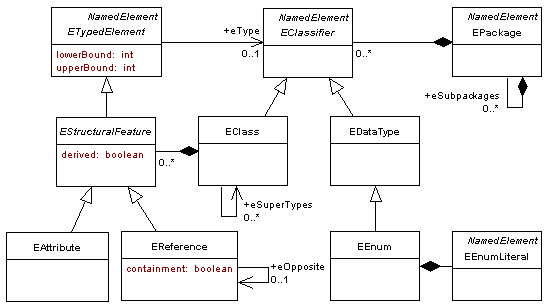
\includegraphics[width=\textwidth]{ecore.png}
\caption{Мета-мета-модель \tool{Ecore}}\label{Ecore}
\end{figure}

На \figref{Ecore} изображена диаграмма мета-мета-модели \tool{Ecore}. Согласно объектно-ориентированной парадигме, центральным понятием в \tool{Ecore} является класс. Экземпляры \tool{Ecore} (то есть мета-модели) представляют собой наборы классов, организованные в пакеты и связанные отношением ``общее-частное'', аналогичным наследованию в объектно-ориентированных языках программирования \cite{OOAD}. На \figref{ComponentClassEcore} показано, как элементы мета-модели, описывающей модели зависимостей между компонентами (такие как \figref{DiagramExample}) связаны с соответствующими мета-элементами в \tool{Ecore}.

//ComponentClassEcore

Следует обратить внимание на то, что \tool{Ecore} сама состоит из классов, что и позволяет ``оборвать'' иерархию мета-уровней, не используя $M^4$ (в действительности, иерархия не обрывается, просто все уровни, начиная с $M^3$ совпадают между собой и содержат только мета-мета-модель, то есть в нашем случае --- \tool{Ecore}).

В этом разделе мы опишем несколько основных концепций, используемых \tool{Ecore} (и другими мета-мета-моделями), которые будут использованы при изложении дальнейшего материала.

\paragraph*{Классы.} Как мы уже отмечали выше, основными элементами мета-моделей, описанных с помощью \tool{Ecore}, являются классы. Каждый класс имеет имя уникальное в пределах пакета, список суперклассов и список структурных элементов, атрибутов и ссылок. Экземпляры классов хранят значения для всех атрибутов и ссылок, объявленных самим классом и всеми его суперклассами (что соответствует наследованию членов классов в объектно-ориентированных языках). Класс может быть помечен как абстрактный. Такой класс не может иметь непосредственных экземпляров, экземпляры могут иметь только его подклассы, не являющиеся абстрактными.

Заметим, что понятие абстрактного класса в \tool{Ecore} является чисто номинальным, никаких технических препятствий к созданию экземпляра класса (таких как, например в \tool{Java} или \tool{C++}) быть не может, поскольку \tool{Ecore} не определяет тела методов. 

\paragraph*{Примитивные типы и перечисления.} Классы --- не единственное средство типизации в \tool{Ecore}, кроме них используются примитивные типы данных (Data Types) и перечисления (Enums). Примитивный тип данных представляет собой именованную сущность, семантика которой либо не фиксируется, либо определяется тем языком программирования, на котором реализовано моделируемое ПО (в случае \tool{Ecore} это \tool{Java}). 

\tool{Ecore} определяет несколько встроенных типов данных, таких как строки, целые и вещественные числа и т. д.

Перечисления --- это типы имеющие конечное множество значений (литералов).

\paragraph*{Структурные элементы классов: атрибуты и ссылки.} Основное отличие классов и примитивных типов данных --- в их назначении. Классы являются типами объектов, из которых состоят модели, а примитивные типы и перечисления --- типами значений атрибутов этих объектов. Таким образом, ссылки, определяемые классами могут иметь в качестве типа только класс, а атрибуты --- только примитивный тип или перечисление.

В остальном ссылки и атрибуты очень похожи. И те, и другие имеют имя и кратность, которая задается как пара чисел, определяющих нижнюю и верхнюю границу для количества значений, хранимых атрибутом или ссылкой. Так, например, ссылка \code{dependsOn} на \figref{DiagramExample} имеет кратность ``от 0 до $\infty$'', что означает, что компонента может зависеть от нуля или более других компонент. Атрибут \code{name} на том же рисунке имеет кратность ``от 1 до 1'', что означает, что каждая компонента должна иметь имя, причем ровно одно.

Как атрибуты, так и ссылки могут быть помечены как ``упорядоченные''. Этот флаг имеет значение для множественных ссылок и атрибутов (верхняя граница кратности которых больше единицы), и означает, что порядок объектов, на которые указывают ссылки (или значений атрибута) важен. Например, в классе \code{Block}, описывающего блок кода в программе и имеющего ссылку \code{statements}, указывающую на последовательность предложений внутри блока, ссылка \code{statements} должна быть упорядоченной, поскольку нам важно знать, в каком порядке выполнять предложения, из которых состоит блок.

\paragraph*{Перекрестные ссылки и агрегация.} Ссылки в \tool{Ecore} подразделяются на два вида: \term{перекрестные} и \term{агрегирующие}. Различие состоит в том, что на один объект не может быть более одной агрегирующей ссылки, то есть объект, имеющий агрегирующую ссылку, ``владеет'' объектом, на который ссылается. Для перекрестных ссылок таких ограничений нет, на любой объект может быть сколько угодно перекрестных ссылок.

Таким образом, если рассматривать модель как граф, ребрами в котором являются ссылки, то любой цикл обязан проходить хотя бы по одной перекрестной ссылке, а агрегирующие ссылки в модели определяют остовный лес \cite{cormen01introduction}.

Явное выделение агрегирующих ссылок позволяет легко представлять модели в древовидной форме, как показано на \figref{ModelTree}.

\begin{figure}[htbp]
\centering
%\includegraphics[width=\textwidth]{model_tree.jpg}
\caption{Представление модели в древовидной форме}\label{ModelTree}
\end{figure}

\paragraph*{Параметризованные типы.} Поскольку \tool{Ecore} развивается на платформе \tool{Java}, с выходом \tool{Java} 5 в мета-мета-модель были добавлены \term{обобщенные типы} (generic types, \cite{GJ}). Любой класс или тип данных может иметь параметры, которые могут служить типами для структурных элементов.

\section{Текстовая нотация для мета-моделей}
//


\chapter{Предметно-ориентированные языки}

Одновременно с мета-моделированием развивается концепция \term{предметно-ориентированных языков (ПОЯ)} (Domain-Specific Languages, DSLs \cite{StateMachine}). В рамках этой концепции утверждается, что во многих предметных областях существуют типичные задачи, для решения которых целесообразно разрабатывать специализированные языки, позволяющие легко выразить специфичные для данной области понятия. ПОЯ противопоставляются \term{языкам общего назначения} (General-Purpose Languages, GPLs), таким, например, как популярные языки программирования (\tool{C}, \tool{C++}, \tool{Java}, \tool{C\#} и т.д.). Задачи, специфичные для данной области, можно решать и с помощью языков общего назначения, но при таком подходе решения получаются гораздо большими по объему и содержат много однотипного кода, который не всегда возможно выделить в библиотеку. Кроме того, поскольку ПОЯ оперируют понятиями предметной области, они становятся более доступными для понимания экспертами в этой области, не имеющими навыков программирования, что облегчает процесс общения с заказчиком и позволяет снизить затраты.

В качестве примеров ПОЯ можно привести
\begin{enumerate}
\item издательскую систему \TeX ;
\item язык разметки \tool{HTML};
\item языки, используемые в конфигурационных файлах, например, для веб-сервера \tool{Apache};
\item язык для вывода графики \tool{PostScript};
\item язык описания графов \tool{GraphViz};
\item нотация EBNF для описания контекстно-свободных грамматик;
\item структурированный язык запросов для реляционных баз данных \tool{SQL};
\item и многие другие.
\end{enumerate}

Некоторые ПОЯ, например \TeX , являются универсальными в том смысле, что с их помощью можно описать любое вычисление, однако они спроектированы так, что с их помощью легко решать задачи в соответствующей предметной области, а описывать другие вычисления --- гораздо сложнее (как правило сложнее, чем на языках общего назначения).

\chapter{Понятие языка}

Несмотря на то, что концепции мета-моделирования и ПОЯ развивались независимо, они тесно связаны между собой, поскольку мета-модели логично рассматривать как языки описания моделей (а мета-мета-модель, соответственно, как язык описания мета-моделей). Таким образом, \tool{Ecore} (MOF, KM3 и т. д.) можно рассматривать как ПОЯ для описания ПОЯ. Эта точка зрения приобретает все большую популярность \cite{}.

Для более глубокого понимания взаимосвязей мета-моделирования и ПОЯ требуется определить само понятие ``язык''. В разных областях математики, логики и компьютерных наук это делается по-разному \cite{???}, например в математической логике термин ``язык'' часто используется как синоним термина ``множество''; нередко имеется в виду множество, описанное определенным образом \cite{}. Здесь и далее мы не будем говорить о языках ``вообще'', а ограничим наше рассмотрение \term{языками моделей}:

\newcommand{\Lang}[1]{\mathcal{L}\left(#1\right)}%
\newcommand{\LMM}[1]{\Lang{\MM{#1}}}%

\begin{Def}
Пусть задана мета-модель $\MM{M}$. Будем называть множество всех моделей, являющихся экземплярами $\MM{M}$, \term{языком, порожденным этой мета-моделью}, и обозначать $\Lang{\MM{M}}$.
\end{Def}

Это определение позволяет описывать как языка моделирования, такие как UML \cite{???}, которые изначально задаются с помощью мета-моделей, так и языки в более традиционном понимании. Например, в теории формальных языков \cite{???} принято определять язык как множество строк над конечным алфавитом; под наше определение подпадают те из языков, определенных таким образом, для которых есть конечное описание в виде (не обязательно контекстно-свободной) грамматики \cite{???}. Мета-модель, соответствующая грамматике состоит из классов, описывающих структуры термов соответствующей индуцированной алгебры \cite{???}.

\ignore{

Для того, чтобы рассуждать о большинстве языков, используемых на практике (например, о языках программирования), ниже мы определяем понятия, связанные с ``синтаксисом'' языков.

\section{Синтаксис}

Понятие ``синтаксис'', чаще всего ассоциируемое с правилами записи предложений языка, является сильно перегруженным и требует внимательного рассмотрения во избежание путаницы в терминах. В данном разделе мы постараемся разделить различные категории понятий, подразумеваемые в разных контекстах под словом ``синтаксис'', и ввести соответствующие определения.

\paragraph*{Конкретный синтаксис. } Способ визуального отображения языка мы будем называть \term{нотацией} (или \term{конкретным синтаксисом}) этого языка.

Для одного и того же множества языка $\LMM{M}$ можно задать несколько (бесконечно много) разных способов отображения. Среди всевозможных нотаций выделяют следующие практически важные классы:
\begin{enumerate}
\item текстовые нотации: предложения языка отображаются в виде строк символов некоторого конечного алфавита;
\item графические нотации: предложения языка отображаются в виде графических изображений, при этом роль играет цвет, форма и толщина линий, взаимное расположение объектов.
\end{enumerate}

Важной разновидностью текстового конкретного синтаксиса является ``расширяемый язык разметки'' (eXtensible Markup Language, XML \cite{XML}), являющийся на сегодняшний день промышленным стандартом для структурирования информации, хранимой в виде текста. Идейным предшественником XML можно считать нотацию S-выражений языка \tool{Lisp} \cite{LISP}.

Формально говоря, текстовый конкретный синтаксис можно считать разновидностью графического, но обычно такая классификация не представляет интереса, хотя в последние годы с появлением псевдо-текстового синтаксиса (системы MPS \cite{MPS}, Amadeus \cite{Amadeus}, SymADE \cite{SymADE}) граница между этими двумя понятиями постепенно стирается.

// Почему мы выбираем текстовый синтаксис? (Надо ли оно?)

Мы будем использовать следующее определение нотации:

\newcommand{\NNot}[3]{#1^{{#2} \rightarrow{} {#3}}}
\newcommand{\Not}[3]{\NNot{#1}{\MM{#2}}{\MM{#3}}}
\newcommand{\N}[2]{\Not{#1}{#1}{#2}}

\begin{Def}
\term{Нотацией} $\N{N}{M}$ для языка $\LMM{M}$ будем называть кортеж, состоящий из следующих объектов:
\begin{enumerate}
\item мета-модель $\MM{N}$;
\item однозначная вычислимая функция $$Meaning_N : \LMM{N} \rightarrow (\{\bot\} \cup \LMM{M}),$$ определенная везде на области задания.
\end{enumerate}

Там, где из контекста ясно, о каких мета-моделях идет речь, мы будем обозначать нотацию как $\Not{N}{}{}$.
\end{Def}

Согласно этому определению, нотация $\N{N}{M}$ задается некоторым множеством $\LMM{N}$ (в случае текстовых нотаций мета-модель $\MM{N}$ просто описывает произвольную последовательность символов, см. \figref{TextMM}), элементы которого преобразуются в элементы языка функцией $Meaning_N$ (в некотором смысле, эта функция выполняет роль, аналогичную роли компилятора языка программирования). Если функция $Meaning_N$ возвращает элемент $\bot$, это означает, что соответствующий элемент нотации некорректен (например, текст программы содержит синтаксическую ошибку).

\begin{figure}[htbp]
\caption{Мета-модель текста}\label{TextMM}
\end{figure}

Для одного и того же языка можно определить несколько нотаций, причем различные нотации не обязаны иметь различные мета-модели. Так, например, текстовых нотаций (заданных одной и той же мета-моделью \figref{TextMM}) для одного языка можно определить бесконечно много (например, добавляя обязательное ключевое слово в начало текста программы).

В широком смысле можно говорить о том, что нотация $\N{N}{M}$, точнее функция $Meaning_N$, определяет \term{денотационную семантику} \cite{???} языка $\LMM{N}$ в терминах языка $\LMM{M}$.

Всякий компилятор можно рассматривать как реализацию функции $Meaning_N$, где нотация $N$ является текстовой. Однако, как правило, компиляторы не работают ``в один шаг'', а выполняют серию преобразований из одной нотации в другую. Так, стандартной последовательностью является (1) преобразование текста в последовательность лексем, далее (2) построение абстрактного синтаксического дерева, которое (3) преобразуется во внутреннее представление, которое, после (4) оптимизации, (5) транслируется в машинный код \cite{Dragon}. Этот процесс можно рассматривать как одну трансформацию из текста в машинный код, а можно выделить в нем не менее пяти указанных этапов, имеющих, каждый, свои входной и выходной языки. Ниже мы часто будем прибегать к такому детализированному рассмотрению.
\newcommand{\Comp}[2]{#1 \circ #2}
\begin{Def}
Нотация $\N{N}{M}$ является \term{композицией} нотаций $\Not{A}{N}{B}$ и $\N{B}{M}$ и обозначается $\Comp{A}{B}$, если 
	$$Meaning_N(n) := \left\{\begin{array}{ll}
		Meaning_{A}(Meaning_{B}(n)), & \mbox{при } Meaning_{B}(n) \neq \bot\\
		\bot, & \mbox{в противном случае}
	\end{array}\right.$$
\end{Def}

Смысл условия в данном определении состоит в том, что если на некотором этапе была обнаружена ошибка ($\bot$), она не теряется, а распространяется на остальные этапы. Поскольку компиляторы следуют этой стратегии (не замалчивают ошибки), описанный выше процесс компиляции можно рассматривать как композицию пяти нотаций.

%На первый взгляд, согласно нашему определению, каждый новый способ отображения дает новый язык, однако такая интерпретация не неудобна с практической точки зрения: многие системы (Intentional \cite{Intentional}, MPS \cite{MPS}, GMF \cite{GMF} и др.) позволяют отображать одни и те же данные разными способами (этот подход называется \term{проективное редактирование}, Projection Editing \cite{Projection}), поэтому целесообразно говорить о том, что те или иные способы отображения относятся к одному и тому же языку (можно считать, что объединение нескольких видов конкретного синтаксиса само по себе является единым способом визуального отображения). 

\paragraph*{Абстрактный синтаксис. } Понятие ``абстрактного синтаксиса'' в литературе трактуется по-разному \cite{Dragon ...}, поскольку существует много различных ``уровней абстракции'' (по сути, различных нотаций, объединенных последовательной композицией).

Так, рассматривая языки с текстовым конкретным синтаксисом, под абстрактным синтаксисом чаще всего понимают алгебру термов, индуцированную грамматикой, описывающей конкретный синтаксис. В этом случае говорят об абстрактных синтаксических деревьях (Abstract Syntax Tree, AST), рассматривая их как деревья разбора, из которых удалены элементы, не представляющие интереса. Текст можно рассматривать как нотацию для языка таких термов, а соответствующую функцию $Meaning$ реализует синтаксический анализатор (обычно, в композиции с лексическим, но не всегда \cite{SGLR}).

Однако при рассмотрении языков с графическим или псевдо-текстовым конкретным синтаксисом  \cite{MPS, ...} под абстрактным синтаксисом понимают множество всех предложений языка, которое как правило явно задается некоторой мета-моделью (сами предложения являются моделями, то есть типизированными атрибутированными графами).

Следует отметить, что трансляторы текстовых языков обычно выполняют (явное или неявное) преобразование AST в граф, когда разрешают имена в программах (так имя переменной преобразуется в ссылку на объявление этой переменной). Таким образом, возникают понятия \term{первичного} абстрактного синтаксиса (First-Order Abstract Syntax, FOAS) и абстрактного синтаксиса \term{высшего порядка} (Higher-Order Abstract Syntax, HOAS). 

Чтобы избежать путаницы, мы будем придерживаться следующих обозначений:

\begin{Def}
Множество $\LMM{M}$ мы будем называть \term{содержанием} нотации $\N{N}{M}$. Мета-модель $\MM{M}$ будем называть \term{целевой мета-моделью} данной нотации.
\end{Def}

\begin{Def}
Понятие \term{абстрактного синтаксического дерева} (AST) имеет смысл только в связи с некоторой контекстно-свободной грамматикой. AST является термом соответствующей индуцированной алгебры, представленным в форме дерева объектов.
\end{Def}

\section{Графические и текстовые нотации}

Для ПОЯ чаще всего применяются...

\paragraph*{Использование графических нотаций при мета-моделировании}

Модели естественно отображать графически: деревья EMF, диаграммы UML

Очень наглядно, но большие диаграммы трудно читать и укладывать.
Для отображения нужны специальные довольно сложные инструменты.

\paragraph*{Преимущества текстового синтаксиса}

Работает даже в консоли. Независимость от инструментов, поддержка обобщенными инструментами (отображение, редактирование, сравнение, контроль версий). Это не работает для XMI из-за ссылок. появилась HUTN, но ей трудно пользоваться.

недостатки текста: надо парсить сложным алгоритмом, поддерживать параллельно структурное представление со ссылками и т.д.

\paragraph*{Псевдо-текстовый синтаксис}

MPS обладает всеми недостатками графического синтаксиса (редактировать и читать чуть проще, да)

\chapter{Ядро нотации и инфраструктурная функциональность}

Интуитивно понятно, что некоторая часть нотации может быть ``избыточной'' в том смысле, ее можно не использовать, сохраняя при этом возможность выразить все предложения языка, выразимые в исходной нотации. Примером таких избыточных элементов могут служить сокращенные формы записи для часто используемых конструкций языка\footnote{часто их называют ``синтаксическим сахаром'' (syntactic sugar \cite{???})}, такие как оператор \texttt{for} в языке \tool{C} \cite{???}, который легко можно выразить через другие операторы. В данном разделе мы вводим для описания таких элементов понятие \term{инфраструктуры} в рамках нотации, и показываем, что многие возможности в языках программирования, ориентированные на повторное использование, могут быть описаны как инфраструктурные.

\newcommand{\Infra}[1]{Infra\left(#1\right)}
\newcommand{\Core}[1]{Core\left(#1\right)}

\begin{Def}
\term{Множеством инфраструктурных элементов} нотации $\N{N}{M}$ называется максимальное по включению множество $\Infra{N}$ элементов мета-модели $\MM{N}$, исключение которого из рассмотрения не сужает образа функции $Meaning_N$:
	$$
		Meaning_N\left[
			\Lang{\MM{N} \setminus \Infra{N}}\right] = Meaning_N[\LMM{N}]
	$$
	
Множество элементов, не являющихся инфраструктурными, будем называть \term{ядром нотации} $N$ и обозначать $\Core{N}$.
\end{Def}

\begin{Def}
	Нотацию, для которой множество $\Infra{N}$ пусто, будем называть \term{минимальной}.
\end{Def}

\begin{Prop}
	Любую нотацию можно представить как композицию $\Comp{A}{B}$, где $B$ является минимальной нотацией.
\end{Prop}
\begin{proof}
Рассмотрим произвольную нотацию $\N{N}{M}$. Если она является минимальной, то она представима в виде
	$$\N{N}{M} = \Comp{\Not{1}{N}{N}}{\N{N}{M}},$$
где $\Not{1}{N}{N}$ --- \term{тождественная} нотация (имеет в качестве содержания самое себя).

Если $N$ не является минимальной, существует нотация $\NNot{\underline{N}}{\Core{N}}{\MM{M}}$, являющаяся минимальной частью $N$: ее можно получить, сузив функцию $Meaning_N$ на ядро нотации $N$. Для каждого предложения $m$ языка $\LMM{M}$ можно выбрать ``каноническое представление'' в нотации $\underline{N}$, то есть элемент $Norm(m) \in \Core{N}$, такой что $Meaning_{\underline{N}}(Norm(m)) = m$.

Теперь рассмотрим нотацию $\NNot{\overline{N}}{\MM{N}}{\Core{N}}$ с функцией
	$$Meaning_{\overline{N}}(n) := Norm(Meaning_N(n)),$$
легко видеть, что $N = \Comp{\overline{N}}{\underline{N}}$.
\end{proof}

Мы показали, что инфраструктурная функциональность может быть выражена статически как трансляция расширенной нотации в минимальную.  Ниже мы покажем, что многие возможности языков программирования, связанные с повторным использованием, могут быть выражены с использованием только инфраструктурных элементов. Это позволяет реализовывать такие возможности отдельно от основных возможностей языка, а также автоматизировать их создание.

Повторное использование всегда базируется на тех или иных механизмах композиции: средствах, позволяющих комбинировать одни и те же объекты многими способами.

// Пояснить

??? В принципе, композиция может поддерживаться не только на уровне инфраструктуры, но и на уровне содержания языка. Например, как мы покажем ниже, модули часто являются элементами инфраструктуры, а функции и классы, также обеспечивающие композицию, имеют динамическую семантику и, следовательно, являются неотъемлемыми элементами содержания языка.

??? Рассмотрим наиболее широко используемые средства композиции, которые как правило обеспечиваются инфраструктурой.

\section{Механизмы идентификации}

Для реализации механизмов повторного использования (композиции) необходимо, чтобы в языке была возможность \term{идентификации} внутри программы, то есть, чтобы из одной части программы можно было сослаться на элемент, определенный в другой ее части. Чаще всего для этой цели используются имена --- уникальные строковые идентификаторы присваиваемые переменным, функциям и т. д., однако нередко используются и более сложные механизмы, например квалифицированные имена (пакет + подпакеты + класс) в \tool{Java} \cite{JLS} или сигнатуры функций при перегрузке в \tool{C++} \cite{???}. Так или иначе, элементам программы сопоставляются \term{идентификаторы} --- объекты, уникальные в определенной области видимости. Важно отметить, что идентификатор не обязан быть уникальным глобально: во-первых, если он уникален в рамках поименованной области видимости, которая, в свою очередь, имеет глобальный идентификатор, этой информации достаточно, чтобы глобально идентифицировать объект; в этом случае мы будем говорить о составном идентификаторе, включающем идентификатор области видимости. Во-вторых, идентифицируемый объект может быть принципиально не доступен из некоторых областей видимости, как, например, локальная переменная, которая ``не существует'' за пределами функции, в которой она объявлена. К таким объектам не должно быть доступа извне, а следовательно и глобальных идентификаторов.

%Наша задача --- показать, что идентификаторы как таковые в большинстве языков являются инфраструктурными элементами нотации. Интуитивно, аргументом в пользу этого является тот факт, что при согласованном переименовании всех упоминаний некоторого элемента в программе, смысл программы (то есть значение функции $Meaning_N$) остается прежним\footnote{Исключением из этого правила являются языки с динамическими возможностями, в частности, поддерживающие \term{рефлексию} \cite{???}.}. В теории функционального программирования такое преобразование называется $\alpha$-редукцией \cite{???}; в силу значительных неудобств, связанных с формализацией $\alpha$-редукции при описании семантики различных $\lambda$-исчислений, были разработаны методы, позволяющие полностью избавиться от имен при описании семантики \cite{HOAS, NomL}.

Пусть $\MM{C}$ --- мета-модель, описывающая машинный код (или язык ассемблера) некоторого процессора или виртуальной машины. Язык $L$, компилируемый для этого процессора или виртуальной машины, можно рассматривать как нотацию $\N{L}{C}$. Эту нотацию можно представить как композицию двух других нотаций: 
$$N{L}{C} := \Comp{\Not{P}{L}{G}}{\Not{Q}{G}{C}},$$
причем в мета-модели 
Ссылки на переменные (вложенные области видимости)
Ссылки на функции и перегрузка
Пространства имен (могут быть и вложенными)
Атрибуты доступа?

\section{Модули}

В большинстве языков программирования \term{модулями} называются фрагменты программ, пригодные для повторного использования путем цитирования: при необходимости обратиться к коду, находящемуся внутри модуля, достаточно ``подключить'' этот модуль в текущей области видимости, после чего можно пользоваться именованными элементами программы, определенными в этом модуле. \cite{???}

Цитирование является, очевидно, простейшим из возможных способов композиции --- одна часть программы просто ссылается на другую. Рассмотрим механизмы работы модулей в различных языках программирования и возможности реализации этих механизмов как инфраструктурных элементов нотации. Нотацию каждого языка мы попытаемся разделить на ядро и инфраструктуру, таким образом, чтобы все, что касается модулей, оказалось в инфраструктурной части.

\paragraph*{Язык \tool{C}. } Вероятно, самая простая реализация модулей принята в языке программирования \tool{C} \cite{???}. Строго говоря, в языке \tool{C} модули вообще не поддерживаются, поскольку обработкой подключаемых заголовков занимается отдельная программа --- \term{препроцессор} \cite{???}, которая способна обрабатывать произвольный текст, размеченный специальными \term{директивами}, а не только код, написанный на языке \tool{C}. 
Однако, поскольку спецификация препроцессора включена в стандарт, и практически никакая программа на \tool{C} не мыслима без его использования, мы будем рассматривать директивы препроцессора как часть нотации языка \tool{C}.

Объявления библиотечных функций и структур данных делаются в отдельных файлах, называемых \term{заголовочными} (header files). Эти файлы, как правило, не содержат реализаций функций, которые помещаются в \term{исходных файлах} (source files). Исходные и заголовочные файлы могут использовать директивы включения \code{\#include}. Препроцессор, обрабатывает исходные файлы по отдельности, вставляя текст включаемых файлов вместо директив включения, пока в тексте есть такие директивы. Таким образом, в результате получается один файл, содержащий все прямо или косвенно включенные объявления, который, в свою очередь, обрабатывается компилятором.

Из сказанного выше видно, что процесс обработки исходного текста включает фазу, которая переводит программу в более богатой нотации (с директивами включения) в программу в менее богатой нотации. Поэтому мы можем рассматривать директивы препроцессора как инфраструктурную часть нотации языка \tool{C}, а отделение препроцессора от компилятора --- как декомпозицию нотаций. 

Вывод: в языке \tool{C} механизм композиции обеспечивается с помощью инфраструктурных элементов нотации. 

\paragraph*{Язык \tool{Pascal}. } В языке \tool{Pascal} \cite{???} модули (units) являются частью основной нотации: каждый модуль имеет имя, которое используется для ссылок на него (в отличие от имени файла в случае \tool{C}), объявления, сделанные в модуле получают идентификаторы в соответствующем пространстве имен, то есть если имена функций, объявленных в разных модулях, совпадают, у программиста есть возможность явно указать, об объявлении из какого модуля идет речь в программе. Сходство с \tool{C} заключается в том, что каждый модуль определяется в отдельном файле, имеется способ подключения модулей, в модуле выделяется интерфейсная часть, в которой, как и в заголовочном файле в \tool{C}, могут содержаться только объявления. Можно сказать, что система модулей \tool{Pascal} гораздо больше контролируется статически, в отличие от \tool{C} (это утверждение верно и при сравнении другой функциональности этих языков). 

Несмотря на то, что в случае языка \tool{Pascal} механизм, обрабатывающий модули, интегрирован в компилятор и не является отдельной программой как препроцессор \tool{C}, мы можем представить нотацию этого языка как композицию двух нотаций, вторая из которых не содержит модулей (то есть реализовать модули как инфраструктурную часть нотации). Функцию $Meaning$ для первой нотации достаточно реализовать аналогично принципу работы препроцессора в \tool{C}: вставить текст модулей в использующие из программы (переименовывая элементы в случае повторений \cite{capture-avoiding-substitution})\footnote{В некоторых случаях будет необходимо добавить предварительные декларации для типов и функций, но это всегда возможно сделать, поскольку \tool{Pascal} запрещает циклические зависимости между интерфейсами модулей}. Программа, полученная в результате не будет содержать следующих элементов: предложений \code{uses} (включений модулей), объявлений модулей (\code{unit interface ... implementation ... end}), имен переменных, функций и типов, квалифицированных именами модулей для разрешения конфликтов (эти элементы будут переименованы).

Вывод: механизм модулей языка \tool{Pascal} можно представить в виде инфраструктурной части нотации.

\paragraph*{Язык \tool{Java}.} Модули, аналогичные тем, что есть в \tool{Pascal} и \tool{C}, в языке \tool{Java} в чистом виде не представлены: функции пространств имен для объявлений выполняют классы, которые также являются объявлениями типов \cite{JLS}. Наиболее близким к традиционным модулям понятием в \tool{Java} является \term{пакет} (package) --- пространство имен, в котором объявляются только типы (классы, интерфейсы, перечисления). Пакеты с модулями роднит в первую очередь механизм \term{импортирования}: чтобы воспользоваться типом, объявленным в другом пакете, программисту необходимо написать предложение \code{import} или квалифицировать имя класса именем пакета.

Если не принимать во внимание динамических возможностей языка \tool{Java} (в первую очередь, библиотеки \code{reflection}, позволяющей обращаться к классам и методам по идентификаторам, записанным в виде строк \cite{JLS}), пакеты можно выразить как инфраструктурную функциональность (аналогично модулям в \tool{Pascal}). Но этот подход воспрепятствует правильной работе механизмов, основанных на динамической загрузке классов, таких, например, как использование одного экземпляра библиотеки несколькими приложениями.

Вывод: механизм пакетов языка \tool{Java} можно выразить с помощью инфраструктуры нотации лишь частично.

\section{Шаблоны}

В предыдущем разделе мы видели, в какой мере модули могут быть выражены как инфраструктура нотации. Общий вывод таков: статическая композиция выражается легко, а динамическая --- не выражается. Это вполне естественно, поскольку само понятие инфраструктуры нотации основывается на \emph{статической} композиции, а не на динамической. Грубо говоря, инфраструктура описывает часть программы, которая может быть полностью вычислена во время компиляции.

Модули представляют собой самый простой механизм композиции. В данном разделе мы рассмотрим механизм \term{макроопределений} (или ``шаблонов''), который, не котором смысле обобщает механизм модулей и предоставляет возможности для более гибкого повторного использования.

\paragraph*{Происхождение термина ``шаблон''.} Термин ``шаблон'' (template) позаимствован из языка программирования \tool{C++} \cite{???}. Этот язык позволяет программисту определять не только классы и функции, но и шаблоны классов и функций --- параметризованные определения, которые можно \term{инстанцировать}, указав значения параметров. Как правило, параметрами являются типы, но можно использовать и константы. Изначально шаблоны были введены в язык для того, чтобы поддержать параметрический полиморфизм \cite{???}, который необходим для реализации удобной библиотеки контейнеров \cite{???}, однако оказалось, что шаблоны позволяют сделать гораздо больше \cite{???}, например, и их помощью можно вычислить во время компиляции любую рекурсивную функцию \cite{???}, то есть компилятор \tool{C++} представляет собой интерпретатор вычислительно универсального языка, основными элементами которого являются шаблоны.

Так или иначе, шаблоны являются частью инфраструктуры нотации языка, поскольку на этапе компиляции каждое упоминание шаблона разворачивается в результате подстановки аргументов на место параметров, и становится обыкновенной функцией или классом. Здесь необходимо заметить, что вследствие вычислительной универсальности шаблонов, процесс их разворачивания может никогда не закончиться (можно написать ``программу'' на шаблонах, порождающую бесконечную цепь рекурсивных обращений шаблонов к самим себе), этот сценарий мы будем считать ошибкой компиляции, то есть функция $Meaning$ для такого входа возвращает $\bot$.

// Haskell \textbf{Template} Meta-programming

\paragraph*{Происхождение термина ``макроопределение''.} Термин ``макроопределение'' (macro-definition или macro\footnote{В некоторых русскоязычных источниках можно встретить слово ``макрос'' (как единственное число существительного мужского рода в именительном падеже), которое образовано транслитерацией слова ``macros'', являющегося формой множественного числа. В силу его грамматической несогласованности, мы избегаем использования этого термина.}) восходит к языкам семейства \tool{Lisp} \cite{???}. Так называется определение в программе, часто --- параметризованное, на которое можно сослаться по имени как на функцию, но оно будет заменено в тексте программы до его выполнения. Например, в языке, где параметры функциям передаются по значению, повторно используемую подпрограмму для обмена переменных местами можно реализовать в виде макроопределения \cite{???}.

\begin{lstlisting}[language=Lisp,label=scheme_swap]
 (define-syntax-rule (swap x y)
    (let ([tmp x])
      (set! x y)
      (set! y tmp)))
\end{lstlisting}

Обращение к этому определению будет заменено на фрагмент программы, меняющий местами значения двух переменных, тогда как вызов функции менял бы местами значения их локальных копий в стеке.

Макроопределения (как и шаблоны) часто используются для создания встроенных предметно-ориентированных языков \cite{???}, поскольку они позволяют в некотором смысле расширить язык программирования новыми конструкциями (то есть, в каком-то смысле, добавить в нотацию новые инфраструктурные элементы).

Очевидны сходства макроопределений \tool{Lisp} с шаблонами \tool{C++}: и те, и другие являются параметризованными фрагментами программ, которые разворачиваются во время компиляции. 

\paragraph*{Обработка идентификаторов при разворачивании макроопределений и шаблонов.}
Разворачивание макроопределений (и шаблонов) связано с проблемой повторения идентификаторов. Если обратиться к макроопределению, меняющему местами значение двух переменных через переменную \code{tmp}, дважды, имя \code{tmp} будет объявлено дважды, что во многих языках вызовет ошибку. В других языках это может привести к изменению значения другой переменной, имя которой случайно совпало с \code{tmp}.

В некоторых системах (как, например, в упоминавшемся выше препроцессоре языка \tool{C}, поддерживающем также и макроопределения) решение этих проблем полностью возлагается на программиста: его внимательность и осторожность. Более совершенные системы гарантируют обнаружение подобных ошибок во время компиляции.

В случае шаблонов \tool{C++} задача относительно проста, поскольку тело шаблона (функция или класс) является пространством имен, поэтому необходимо лишь отслеживать отсутствие повторений в именах шаблонов, а также обеспечить различение результатов развертывания с различными параметрами. Так, компилятор считает использования одного и того же шаблона класса \code{std::vector<int>} и \code{std::vector<string>} разными типами, несмотря на то, что имя шаблона повторяется. Таким образом, идентификатором результата развертывания является имя шаблона и его аргументы. При многократном упоминании одного и того же идентификатора (например, \code{std::vector<string>}) шаблон разворачивается только один раз. Можно говорить о том, что в \tool{C++} проблема именования при развертывании шаблона решена \emph{ad hoc}, за счет ограничения набора элементов, которые могут быть результатом развертывания.

В \tool{Lisp}\footnote{Речь идет о семействе \tool{Lisp} 2 \cite{???}} эта проблема решается в более общем виде: с помощью \term{генерирования свежих имен} и \term{гигиены}. Генерирование свежих имен реализовано специальной операцией \code{gensym}, которая порождает имя, не занятое в текущей области видимости. ``Гигиеной'' (hygiene) называется система средств, позволяющих во время развертывания макроопределения проверять, определено ли уже то или иное имя, и переименовывать элементы в случае необходимости.

// Подробнее



Те же модули, но с параметрами (полиморфные или обобщенные)
	то есть включение, но с внедрением пользовательской информации. Контроль на стороне клиента
	LISP
	макросы в C
	С++
	m4/ST/Vel
	Haskell Template Meta-programming
	Nemerle
	Macros as MultiStage Computations: TypeSafe,Generative, Binding Macros in MacroML
}	
\section{Аспекты}

Если смотреть на модули и шаблоны (макроопределения) как на механизмы композиции, они являются последовательными этапами на пути придания гибкости процессу комбинации фрагментов программы. Пусть есть два фрагмента: M (от Main, основная программа) и L (jn Library, библиотека), и M должен использовать часть функциональности L. В этом случае, при использовании простых модулей, M должен выбрать фрагменты L, которые ему нужны, и использовать их. В случае шаблонов, M не только выбирает нужные ему фрагменты, но и может модифицировать их, подставляя собственные значения шаблонным параметрам. Сказанное иллюстрируется \figref{Composition}.

\begin{figure}[htbp]
// Картинка: кружочек, кружочек с дырками, подписано, что L, а что M
\caption{Виды композиции}\label{Composition}
\end{figure}

Развитие этой линии приводит нас к следующему механизму композиции: M вообще не обязан выбирать сам, L может самостоятельно определить, каким частям программы понадобятся те или иные элементы. Такой механизм является дополнительным к описанным выше; он лежит в основе \term{аспектно-ориентированного программирования} (АОП, \cite{???}).

\paragraph*{Язык \tool{AspectJ}.} АОП получило распространение благодаря языку \tool{AspectJ} \cite{???}, созданному на основе \tool{Java}, добавляя конструкции для нового способа композиции (сразу видно, что речь во многом идет об инфраструктурной функциональности). Основными концепциями в новом языке стали \term{точки присоединения} (join points), \term{срезы} (point-cuts) и \term{советы} (advice). Все эти элементы определяются внутри структурных элементов, называемых \term{аспектами}. Аспекты определяют в себе черты классов, объединяющих взаимосвязанные функции и данные, и модулей, хранящих независимые элементы, одновременно.

Аспектно-ориентированная композиция заключается в том, что код \term{совета} встраивается в основную программу. Например, для записи информации о ходе выполнения в журнал, требуется вписать однотипный код во множество мест в программе. Аспекты позволяют решить эту задачу, написав необходимый фрагмент кода только один раз.

Позиции, в которые код может встраиваться, называются \term{точками присоединения}. В \tool{AspectJ} это позиции перед и после вызовов функций, присваиваний, создания объектов и т. д. Для того, чтобы присоединить \term{совет} сразу ко множеству точек, это множество задается с помощью выражений, называемых \term{срезами}. Срезы описывают статическое или динамическое положение точки в программе, например ``вызов метода a()'' или ``создание объекта класса, имя которого начинается на A, которое происходит в потоке управления метода x()''. При присоединении \term{совета} к срезу указывается относительное положение: \term{совет} может присоединяться \term{до} (before), \term{после} (after) или \term{вместо} (around) каждой точки присоединения, соответствующей срезу.

Частным случаем такого подхода является добавление аспектом полей и методов в существующие классы, причем исходный код самих этих классов не изменяется. Этот механизм носит название ITD (Inter-Type Declarations). Например, специальный аспект может реализовывать методы \code{toString} для нескольких классов в одном файле, объединяя таким образом эту функциональность в одном модуле:

\begin{lstlisting}[language={[AspectJ]Java}]
aspect ToString {
	public String A.toString() {
		return "A: " + data;
	}

	public String B.toString() {
		return "B: " + data;
	}

	public String C.toString() {
		return "B: " + data + " " + moreData;
	}
}
\end{lstlisting}

\paragraph*{Характеристические свойства АОП.} С момента появления языка \tool{AspectJ} разработано множество концепций, так или иначе ``напоминающих'' идеи, заложенные в этом языке. В 2000 году в работе \cite{Obliviousness} была предпринята попытка выработать определение АОП, чтобы иметь эффективный критерий, позволяющий сказать, является ли данный язык аспектно-ориентированным. Название работы говорит само за себя: ``Aspect-oriented programming is quantification and obliviousness''\footnote{\textit{(англ.)} Аспектно-ориентированное программирование --- это квантификация и незнание.}
Под \term{квантификацией} (quantification) понимается возможность охарактеризовать множество точек присоединения предикатом, записанном на специальном языке. Под \term{незнанием} (obliviousness) подразумевается, что программа, в которою встраиваются \term{советы}, не знает о том, что они есть, то есть никак не зависит от их кода (код советов может зависеть от кода этой программы).

Таким образом, можно говорить о том, что аспекты --- это ``шаблоны наоборот'': не M использует L, дополняя ее своими фрагментами, а L ``сама'' встраивается в M.

\paragraph*{Аспекты как инфраструктурная функциональность.} \tool{AspectJ} статически компилируется в байт-код платформы \tool{Java}\footnote{Это не единственный способ присоединения аспектов к \tool{Java}-программам. Кроме него поддерживается \term{динамическое встраивание}, при котором байт-код модифицируется при загрузке классов во время выполнения}, из которого можно однозначно восстановить исходный код Java-программы. Это преобразование можно представить как трансформацию кода \tool{AspectJ} в код на \tool{Java} с последующей компиляцией. То есть аспекты можно реализовать как элемент инфраструктуры нотации \tool{AspectJ}.

// Не сказать ли про другие языки?


Сложные правила композиции (взаимопроникающие модули, инвазивная композиция): внедрение доп. информации без ведома клиента (слабее зависимости), прозрачность и т.д.
	
	AspectJ, терминология
	АПОЯ
		примеры для разных доменов
		примеры для грамматик


\section{Распространение рассмотренных механизмов композиции}

табличка: что где есть

мы рассмотрели вот эти языки. эти фичи есть почти везде, значит их приходится часто реализовывать, значит это надо автоматизировать.

\section{Диалекты}

// Рассказать про задачу разработки диалектов трех типов
// Сослаться на статьи про эволюцию языков


%\chapter{Инструменты для автоматизации разработки текстовых языков}

В данном разделе мы рассматриваем существующие инструменты, автоматизирующие разработку языков. В основном, эти инструменты ориентированы на разработку предметно-ориентированных языков, поскольку такие языки необходимо разрабатывать часто, что делает затраты на реализацию даже элементарных возможностей таких языков часто повторяющимися, в результате чего возникает необходимость в максимальном сокращении таких затрат.

В первую очередь нас интересует, насколько существующие подходы позволяют автоматизировать поддержку механизмов композиции, описанных выше, однако мы будем также отмечать и другие особенности этих подходов, в частности, поддержку механизмов композиции в языках, используемых самими инструментами.

\ignore{
\section{Контекстно-свободные грамматики}

--- Описание грамматик
	BNF
	EBNF (шаблоны)
	
	КСГ
	продукция 
	правило 
	правая часть 
	символ 
	терминал 
	нетерминал

	индуцированная алгебра термов
	частичный тип

\section{Атрибутная трансляция}

определения
JustAdd, ITD в нем

	атрибут
	семантическое действие

\section{Синтаксически-управляемая трансляция}

недостаток АТ

определение СУТ, L-атрибутные определения

Генераторы на основе СУТ
	Yacc/Bison и компания
		LALR, только синтез. аттр
	ANTLR
		LL, и те, и те
		
	внедренные семантические действия
}				
\section{Внутренние ПОЯ}

Часто ПОЯ разделяют на \term{внешние} (external) и \term{внутренние} (internal) \cite{StateMachine}. Внешними называют языки, имеющие специальные средства обработки, например, транслятор, написанные именно для данного ПОЯ. Внутренние языки, напротив, не имеют специальных средств обработки: они ``встраиваются'' в языки общего назначения, как библиотеки или расширения другого рода. В принципе, любой прикладной программный интерфейс (Application Programing Interface, API) можно рассматривать как внутренний ПОЯ: функции API выполняют роль ``ключевых слов'' внутреннего языка. Как правило, о внутренних языках говорят, если соответствующий язык общего назначения позволяет обращаться к библиотекам, используя достаточно гибкие синтаксические конструкции.

// Пример про fluent interfaces

Популярными языками для встраивания ПОЯ являются, например, \tool{Groovy} \cite{Groovy}, \tool{Haskell} \cite{Haskell98}, \tool{Scala} \cite{Odersky2008} и \tool{Java} \cite{JLS}. Существуют языки, имеющие специальные механизмы для расширения синтаксиса, позволяющие очень удобно интегрировать внутренние языки, например, \tool{Nemerle} \cite{Nemerle} и \tool{PLOT} \cite{PLOT}.
		
\section{Модульность грамматических определений}

Как ни странно, далеко не все популярные инструменты поддерживают повторное использование грамматических определений, например, \tool{Bison} \cite{BisonBook}, \tool{CoCo/R} \cite{CocoR} и \tool{JavaCC} \cite{JavaCC} не поддерживают никаких механизмов такого рода. Это связано в первую очередь с тем, что грамматические определения ``двумерны'': они содержат как описание синтаксической структуры (продукции КСГ), так и описание вычислений (семантические действия), что затрудняет композицию. Кроме того, специальные классы грамматик (например, $LL(k)$) не замкнуты относительно объединения, что накладывает дополнительные трудности на композицию \cite{???}. Так или иначе, инженерная дисциплина при разработке трансляторов находится на гораздо более низком уровне, чем при разработке других видов ПО \cite{Grammarware}.

В данном разделе мы рассмотрим механизмы повторного использования грамматических определений, основанные на цитировании, то есть модули и шаблоны. Аспектно-ориентированная композиция грамматик рассматривается в следующем разделе.

\subsection{Модули и ограничение видимости} В работе \cite{SysProg-2006} приведен обзор наиболее популярных средств для разработки трансляторов и выполнено сравнение по нескольким критериям, одним из которых является повторное использование.

Простейшая реализация модулей представлена в инструментах \tool{Elkhound} \cite{Elkhound} и \tool{ANTLR} версии 3 \cite{ANTLR}, который поддерживает директиву \code{include} для подключения определение из других файлов. 

Несколько иной подход использован в генераторе \tool{Menhir} \cite{Menhir}, который, принимая на вход несколько файлов, просто ``склеивает'' их содержимое вместе, но позволяет контролировать, какие символы являются открытыми (public) и могут быть использованы в других файлах, а какие --- нет. Закрытые (private) символы автоматически переименовываются для того, чтобы избежать коллизий. Особенность идеи ``склеивания'' файлов состоит в отсутствии директивы цитирования (\code{include} или \code{import}), что облегчает реализацию механизма, но делает зависимости между модулями \emph{невидимыми}: читая отдельный файл, трудно понять, какие из упоминаемых символов определены в других модулях, а главное --- нет никакой возможности определить, в каких именно модулях они определены.

Более традиционным образом модули организованы в системе \tool{ASF+SDF} \cite{ASF+SDF}: аналогично подходу, принятому в языках программирования, каждый модуль имеет имя, соответствующее имени файла, в котором он определен, элементы, объявленные в модуле, делятся на открытые (\code{exports}) и закрытые (\code{hidden}), причем другие модули могут использовать только открытые элементы, что обеспечивает инкапсуляцию. Директива цитирования \code{import} позволяет подключать модули друг к другу. При импортировании может оказаться, что символ, объявленный в одном модуле имеет то же имя, что и символ объявленный в другом. Как мы видели выше, в некоторых языках эта проблема решается с помощью квалифицированных имен (среди инструментов разработки трансляторов такого подхода придерживается \tool{Rats!} \cite{Rats!}); в \tool{ASF+SDF} используется другой подход: директива цитирования позволяет при необходимости \term{переименовать} символ, импортируемый из данного модуля, например:

\begin{lstlisting}
module example/Example

imports library/Lib[ A => B ]
\end{lstlisting}

Теперь внутри модуля \code{example/Example} символ \code{A}, определенный в \code{library/Lib} будет иметь имя \code{B}.

\subsection{Наследование в грамматических определениях}
% Compiler generation based on grammar inheritance
Идея \term{наследования грамматик} была впервые предложена в работе \cite{GInh}, и основывается на том, что грамматика может наследоваться от другой грамматики, добавляя новые правила и переопределяя старые. Первоначальная реализация была выполнена на языке \tool{Smalltalk} для рабочей станции \tool{Sun 3}, и не получила широкого распространения, однако в дальнейшем наследование грамматик было реализовано в других инструментах.

В \tool{ANTLR} версии 2 \cite{ParrQ95} наследование грамматик является единственным механизмом их повторного использования. Грамматика может быть унаследована от не более, чем одной родительской грамматики, при этом возможно переопределение правил, а именно: изменение семантических действий (при сохранении синтаксической структуры),  добавление новых альтернатив к существующим правилам. Кроме переопределения, также можно определять и совершенно новые правила (которые могут ссылаться на символы, определенные в родительской грамматике). К недостаткам такого подхода к повторному использованию можно отнести тот факт, что наследование является одиночным, и у разработчика нет возможности использовать несколько независимых модулей при разработке одного языка. Создатели \tool{ANTLR} 2 в качестве основного сценария использования наследования грамматик указывали создание нескольких диалектов одного языка \cite{???}.
% http://www.antlr2.org/doc/inheritance.html

Множественное наследование атрибутных грамматик предложено в работе \cite{MAGInh} и реализовано в инструменте \tool{LISA}. %http://portal.acm.org/citation.cfm?id=606666.606678
Авторы уделили больше внимание повторному использованию семантических действий, но и синтаксическая структура может быть унаследована, дополнена и частично переопределена.
Важным дополнением к наследованию грамматик в \tool{LISA} являются \term{шаблоны}.

В некоторых объектно-ориентированных языках (таких, например, как \tool{Scala} \cite{Odersky2008}) альтернативой наследованию является ``подмешивание'' (mixins). Похожий механизм для грамматик реализует инструмент \tool{xText} \cite{xText}. Результирующий механизм близок к множественному наследованию грамматик, но более строго и просто определяет поведение системы в случае ``ромбовидного наследования'' \cite{C++}. Mixin в \tool{xText} может добавлять новые правила или продукции, а также переопределять существующие.

Единственным известным нам инструментом, позволяющим не только добавлять, но и удалять продукции, является \tool{Rats!} \cite{Rats!}. Этот инструмент не используем явным образом метафору наследования для грамматик: авторы говорят лишь о ``модификации импортируемых модулей'', однако функциональность, реализованная этой операцией схожа с тем, что в других инструментах достигается с помощью наследования грамматик: есть возможность добавить продукцию, заменить или даже удалить ее.


\paragraph*{Параметризованные определения (шаблоны).}
Идею использования шаблонов (макроопределений для продукций или правил) при описании формальных грамматик легко проиллюстрировать на следующем примере: в синтаксисе языков программирования очень часто встречаются списки --- последовательности элементов (например, имен переменных), разделенных специальным символом (например, запятой). Элементы и разделители разнятся в зависимости от контекста. В грамматике языка \tool{Java} \cite{JLS} такие конструкции встречаются не менее 14 раз. Для того, чтобы решить проблему списков однажды и навсегда, можно определить следующий шаблон:

\begin{lstlisting}
	list<item, sep> -> item (sep item)*;
\end{lstlisting}

В результате возникает возможность коротко описывать такие разные языковые конструкции как вызов функции и арифметическое выражение:

\begin{lstlisting}
	functionCall -> NAME '(' list<expression, ','> ')';
	arithExpr -> list<product, plusOrMinus>;
\end{lstlisting}

Действительно, в скобках при вызове функции указывается список выражений, разделенных запятыми, а арифметическое выражение --- это алгебраическая сумма произведений, то есть список произведений, разделенных плюсами или минусами.

Стандартизированная нотация EBNF \cite{EBNF} имеет поддержку таких несложных шаблонов, хотя большинство инструментов реализует шаблоны по-своему. Прообразом грамматик с шаблонами можно считать двухуровневые грамматики \cite{???} использованные при описании \tool{Algol68} \cite{Algol68}, однако они не получили широкого распространения: идея была упрощена и приспособлена для понимания инженерами.

Реализация шаблонов в \tool{Menhir} наиболее близка к требованиям стандарта EBNF: индивидуальные правила могут иметь параметры, которым сопоставляются значения при использовании. В \tool{LISA} поддерживаются шаблоны для семантических действий: параметрами являются вхождения атрибутов.

Еще один способ использования шаблонов при описании грамматик состоит в определении не отдельных правил или продукций с параметрами, а в параметризации целой грамматики. Этот подход может служить хорошей альтернативой наследованию грамматик (он, фактически, аналогичен \term{делегированию} в объектно-ориентированных языках \cite{Gamma1995}). Например, грамматика, определяющая арифметические выражения, может принимать синтаксическую форму для атомарных выражений в виде параметра:

\begin{lstlisting}
grammar template Arith<atom> {
	sum    -> mult (('+' | '-') mult)*;
	mult   -> factor ('*' factor)*;
	factor -> '(' sum ')';
	       -> <atom>;
}
\end{lstlisting}

Этот шаблон позволяет порождать грамматики для арифметических выражений над разными (атомарными) объектами, например, над целочисленными константами и переменными:

\begin{lstlisting}
grammar Arith<INT | VAR>;

INT -> [0-9]+;
VAR -> [a-zA-Z_][a-zA-Z_0-9]*;
\end{lstlisting}

Или над комплексными константами:

\begin{lstlisting}
grammar Arith<complex>;

complex -> '(' FLOAT ',' FLOAT ')';
FLOAT   -> INT '.' INT;
\end{lstlisting}

Параметризацию модулей поддерживают инструменты \tool{ASF+SDF} и \tool{Rats!}, но эти возможности реализованы в них по-разному. \tool{Rats!} позволяет использовать в качестве параметров только модули целиком: параметризованный модуль может импортировать модуль-параметр и обращаться к символам внутри этого модуля. Такой подход в наибольшей степени схож с идеей делегирования в ООП: модуль рассматривается как класс, а набор имен символов --- как интерфейс\footnote{Здесь правомерно говорить об аналогии со ``статическим полиморфизмом'' в \tool{C++} \cite{C++}.}. В \tool{ASF+SDF}, напротив, модуль не может быть параметром, в качестве таковых используются только отдельные символы. 

Оба подхода имеют свои недостатки: в \tool{Rats!}, чтобы передать всего один символ в качестве параметра, придется создать модуль, а в \tool{ASF+SDF} неудобно передавать много символов за один раз. Кроме того, шаблоны отдельных правил и выражений в этих инструментах создавать нельзя. Нам не известно о существовании инструмента, поддерживающего все три способа параметризации.
	
\section{Аспектно-ориентированные грамматические определения}

Следующим шагом в развитии средств повторного использования грамматических определений является поддержка аспектов.

// Переписать рассуждения про то, откуда croscutting concerns в грамматиках
// Добавить объяснения про то, что grammar duplication и entanglement при генерации специфических тулов

% Separation of concerns in compiler development using aspect-orientation --- 2006
В работе \cite{Wu06} отмечается, что даже использование аспектно-ориентированного языка общего назначения (\tool{AspectJ}) облегчает разработку трансляторов. Многие инструменты интегрировали поддержку аспектов с более традиционной функциональностью, описанной выше.

Широкую известность получил подход, использованный в системе \tool{JastAdd} \cite{JastAdd}, основанной на расширенном определении атрибутных грамматик. В рамках этого подхода (использованного также и в других работах, см. \cite{Silver}) типы вершин AST рассматриваются как классы, а атрибуты определяются как методы с помощью механизма ITD.

Системы \tool{Silver} \cite{Silver} и \tool{AspectLISA} \cite{LISA} также используют аспекты для присоединения семантических действий к продукциям грамматики. Однако, если \tool{JastAdd} позволяет ссылаться лишь на имена символов и не имеет, строго говоря, механизма срезов (point-cuts), что делает квантификацию (см. раздел ???) довольно примитивной, то эти инструменты уже используют срезы для определения точек присоединения. \tool{Silver} позволяет цитировать целиком текст продукции, что гораздо слабее полноценного механизма срезов, используемого в \tool{AspectLISA}: этот инструмент позволяет использовать подстановочные знаки и параметры при определении срезов, аналогично тому как это сделано в \tool{AspectJ} \cite{AspectJ}.

Механизм срезов присутствует и в расширении \tool{ASF+SDF}, названном \tool{AspectASF} \cite{AspectASF}. Этот язык реализует вычисления над AST с помощью переписывающих правил \cite{TermRewriting}; срезы сопоставляют левые части и имена правил, а советы позволяют расширить функциональность, добавляя действия либо перед, либо после обработки правила.

\tool{AspectG} \cite{AspectG} также поддерживает срезы. Этот язык является аспектно-ориентированным расширением входного языка генератора \tool{ANTLR} \cite{ANTLR}. Особенность \tool{AspectG} состоит в том, что он поддерживает срезы, описывающие как грамматическую структуру, так и код семантических действий. Необходимо заметить, что семантические действия в \tool{ANTLR} задаются в виде простых строк, структура которых практически не анализируется, поэтому срезы для таких действий основываются на поиске образца в строке. Советы в \tool{AspectG}, как и рассмотренных ранее инструментах, позволяют только добавлять семантические действия, не изменяя грамматической структуры.

Полноценную модификацию грамматической структуры, как было отмечено выше, позволяет только \tool{Rats!}. Механизм использованный в этом инструменте можно описать как аспектно-ориентированный, основанный на примитивных срезах: все продукции в \tool{Rats!} поименованы, и обращение происходит по имени продукции.

% JastAdd vs Polyglot: Modularity First: A Case for Mixing AOP and Attribute Grammars '08

% AspectG va AspectLisa: Domain-specific aspect languages for modularising crosscutting concerns in grammar

\section{Выводы}

// Добавить мотивацию для Grammatic

Приведенный выше обзор показывает, что, несмотря на то, что всевозможные механизмы композиции успешно опробованы в разных инструментах, автоматизирующих разработку текстового синтаксиса, ни один из них не поддерживает одновременно все наиболее успешные методы композиции, а именно:
\begin{enumerate}
\item модули с поддержкой атрибутов видимости;
\item шаблоны всех элементов нотации (не только модулей, и не только выражений), параметризуемые любыми элементами нотации (не только модулями, и не только символами);
\item аспекты, поддерживающие полноценные срезы, и позволяющие не только оперировать семантическими действиями, но и модифицировать правила грамматики.
\end{enumerate}

Появление инструмента, поддерживающего все эти возможности, удовлетворило бы одновременно потребности разработчиков очень многих языков. Разработка такого инструмента входит в задачи данной работы.

	
\chapter{Автоматизация разработки механизмов композиции}

Из предыдущего раздела видно, что предметно-ориентированные языки (в данном случае --- языки, предназначенные для описания текстового синтаксиса) нуждаются в инфраструктурной функциональности, обеспечивающей композицию, не меньше, чем языки общего назначения. В данном разделе мы рассмотрим инструменты, позволяющие в той или иной степени автоматизировать разработку такой функциональности для предметно-ориентированных языков.

\section{Анализ идентификаторов}

Идентификация элементов является тривиальной задачей для средств разработки графического синтаксиса, поскольку они хранят элементы моделей как объекты в памяти, и могут использовать естественную индивидуальность (identity \cite{OOAD}) этих объектов для идентификации. При сохранении на диск в формате XMI \cite{XMI} также существует стандартизированный механизм идентификации, но получающееся таким образом текстовое представлением неудобно для чтения человеком. Ситуация не облегчается и стандартной нотацией HUTN \cite{HUTN}, поскольку ее синтаксис достаточно громоздок и не очень далек от XMI.

При разработке текстового синтаксиса анализ идентификаторов является третьим этапом создания транслятора \cite{DragonBook}, после лексического и синтаксического анализа. В простых случаях этот механизм легко реализуется с помощью таблицы символов, более сложные случаи требуют усложненных структур данных. Дополнительные трудности накладывает наличие различных пространств имен (например, когда множество имен функций может пересекаться с множеством имен переменных, потому что из синтаксиса всегда ясно, идет ли речь о переменной или о функции) и вложение этих областей. Основанный на атрибутной трансляции инструмент \tool{Eli} \cite{Eli} предоставляет обширную библиотеку для реализации различных вариаций механизма разрешения идентификаторов, но использование этой библиотеки по-прежнему требует написания достаточно большого объема кода.

Генераторы сред разработки, такие как \tool{xText} \cite{xText} и \tool{TCS} \cite{TCS} автоматизируют разрешение имен в простых случаях. \tool{TCS} позволяет определять вложенные области видимости и непересекающиеся пространства имен с помощью специальных директив внутри грамматического определения. 

\section{Механизмы простого цитирования}

Как отмечалось выше, самым простым механизмом композиции являются модули, не использующие параметризацию. Этот механизм позволяет объединять элементы, имеющие идентификаторы, в группы, называемые \term{модулями}. Такой модуль может быть \term{подключен} в некоторой области видимости (как правило в другом модуле), что позволяет использовать объявленные в нем элементы в этой области видимости.

Ряд инструментов, автоматизирующих разработку языков, позволяет добавлять поддержку модулей достаточно легко. Так, инструменты, опирающиеся на графический или псевдотекстовый синтаксис \cite{EMF, Fujaba, MPS} используют для реализации модулей ссылки между моделями, поддерживаемые мета-мета-моделями, использующими XMI \cite{XMI} (например, MOF или \tool{Ecore}), что не требует от разработчика описывать модули дополнительно. Вместе с тем, такая реализация модулей достаточно примитивна, например, она не позволяет вводить \term{атрибуты доступа}, то есть разделять элементы модуля на внутренние (private) и внешние (public).

Для языков с текстовым синтаксисом поддержка модулей реализуется несколько сложнее. Так упоминавшийся выше инструмент \tool{Eli} \cite{Eli} предоставляет библиотеку для реализации нескольких вариантов этого механизма, однако ее использование требует написания большого количества кода. Гораздо более простая реализация имеется в \tool{xText} \cite{xText}: этот инструмент предоставляет ``текстовую оболочку'' для механизма ссылок между моделями, реализованного в \tool{Ecore}, а именно распознает специальное имя атрибута (\code{importURI}) и интерпретирует его как однородный идентификатор ресурса (Uniform Resource Identifier, URI \cite{uri}), который автоматически загружается в текущую область видимости. Как следует из сказанного выше, такой механизм не имеет автоматической поддержки для атрибутов доступа.

Инструменты, позволяющие более полную автоматизацию поддержки модулей, нам не известны, однако ниже мы рассматриваем системы, частично автоматизирующие поддержку шаблонов. Поскольку модули, как мы видели выше, легко представить в виде шаблонов без параметров, можно считать, что средства описания шаблонов поддерживают также и модули.

\section{Шаблоны и макроопределения}

Автоматически шаблоны или макроопределения поддерживают только внутренние (internal) ПОЯ, определенные в языках с поддержкой соответствующих конструкций, таких как \tool{Lisp} или \tool{MacroML}.

Для самостоятельных языков поддержку шаблонов автоматизируют инструменты \tool{COMPOST} \cite{COMPOST} и \tool{Reuseware} \cite{Reuseware}. Последний является развитием первого, поэтому здесь мы опишем только его возможности.
 
Принцип, на котором основывается \tool{Reuseware} его авторы называют инвазивной композицией ПО (Invasive Software Composition, ISC \cite{ISC}). Это методология, определенная для моделей и КС-грамматик, базирующаяся на введение в структуру языка дополнительных элементов, так называемых \term{точек изменения} (variation points), которые подразделяются на следующие типы:
\begin{itemize}
\item \emph{slot} --- помечает выражение в языке для последующей замены, аналогично параметру шаблона со значением по умолчанию \cite{C++};
\item \emph{hook} --- помечает позицию для вставки элементов (возможно, многих), аналогично простому шаблонному параметру;
\item \emph{anchor} --- помечает выражение идентификатором, на который в дальнейшем можно сослаться при описании композиции (см. ниже).
\end{itemize}

Предложения, содержащие точки изменения, называются \term{фрагментами} (Component Fragment). Располагая набором фрагментов, разработчик может описывать их \term{композицию} с помощью специального языка, который определен в инструментах \tool{Reuseware} и имеет графический синтаксис. Композиция заключается в соединении элементов типа \emph{anchor} с элементами двух других типов, причем при присоединении к элементу типа \emph{slot} происходит замена его содержимого, а в случае элемента типа \emph{hook} --- дополнение.

Важной особенностью механизма ISC является тот факт, что он контролирует структурную корректность результата: точки изменения имеют типы (соответствующие классам в мета-модели или нетерминалам в грамматике), и соединение точек с несовместимыми типами запрещено семантикой языка описания композиции, что позволяет гарантировать, что результат не нарушает требований, наложенных целевой мета-моделью. Как мы увидим ниже, те же принципы можно использовать для автоматизированной реализации поддержки аспектов.

Недостатком такого подхода является тот факт, что он \term{незамкнут}: для того, чтобы использовать ``шаблоны'', определенные таким образом, нужно привлекать дополнительный язык, зависящий в свою очередь от инструментов \tool{Reuseware}, то есть расширенная версия исходного языка теряет самостоятельность. Кроме того, способ организации точек изменения гораздо менее локален по сравнению с традиционными шаблонами: ``телом шаблона является вся программа'', что затрудняет инкапсуляцию и делает весь подход менее интуитивным, поскольку теряется аналогия шаблонов с функциями, вычисляемыми во время компиляции \cite{MacroML}.

\section{Аспекты}

Разработку поддержки аспектов в той или иной мере автоматизируют несколько инструментов и методологий. Мы начнем с применения инструментария \tool{Reuseware}, рассмотренного в предыдущем разделе.

Система фрагментов и точек изменения может быть рассмотрена как ``заготовка'' для аспектной композиции. Обеспечить полное \term{незнание} (см. ???) не удается, поскольку точки изменения отмечаются явно, но некоторая степень незнания все же достигается за счет использования внешнего языка композиции. \term{Квантификацию} позволяет обеспечить механизм \term{запросов} (fragment queries), позволяющий коротко описывать множества точек изменения. Этот механизм выполняет функцию срезов. Поиск точек изменения осуществляется по фрагменту имени и типу.  Достоинства этого подхода --- в его универсальности, а недостатки применительно к данной задаче --- в первую очередь, в отсутствии незнания.

Альтернативный подход представлен в работе \cite{VanWyk03}, которая основана на атрибутной трансляции и переписывании. AST, созданное в процессе разбора программы может быть переписано в соответствии с декларативно заданными правилами. При этом поддерживается с \term{перенаправление} атрибутов (forwarding). Идея перенаправления состоит в том, что атрибут элемента AST может быть вычислен путем обращения к атрибуту элемента, полученного в результате переписывания исходного. В такой среде аспекты реализуются следующим образом: срез является предикатом, который определяет применимость того или иного совета для каждого элемента AST (в рамках данного подхода срезы реализуются как функции высшего порядка, написанные на языке Haskell), советы добавляются в код посредством создания новых правил переписывания, а перенаправление позволяет распространить семантические проверки на добавленный таким образом код. Преимуществом этого подхода является возможность добавить аспекты в любой язык независимо от других расширений, причем гарантируется сохранение корректности статических проверок. Основным недостатком является необходимость написания срезов на языке общего назначения, что, как и в случае \tool{Reuseware} делает систему незамкнутой.

Работа \cite{Bagge06} описывает метод, основанный на использовании системы \tool{Stratego/XT} \cite{Stratego/XT} --- широко известного инструмента для трансформации программ, основанного на \emph{стратегическом программировании} (strategic programming), представляющем собой объединение возможностей логического программирования и переписывания термов. Основная идея состоит в том, чтобы описывать применение аспектов как трансформации, во многом аналогично работе \cite{VanWyk03}. В данном случае авторы предлагают вручную реализовать и синтаксис, и семантику аспектов, демонстрируя, что это достаточно легко сделать, располагая инструментами \tool{Stratego/XT} и реализацией самого исходного языка. Строго говоря, эта работа описывает не технологию автоматизации, а метод ручной разработки.

Мы отмечали отсутствие поддержки срезов как недостаток описанных выше подходов. Методология автоматизированного построения системы срезов (но не остальных необходимых элементов аспектного языка) описана в работе \cite{XCPL}. Авторы предлагают использовать ``универсальный'' язык срезов \tool{XCPL}, позволяющий выразить очень широкий класс предикатов над программными конструкциями. Этот язык предлагается сокращать по мере надобности для описания срезов для каждого конкретного языка, при этом необходимо каждый раз разрабатывать конкретный синтаксис сокращенного языка. Семантика \tool{XCPL} также не фиксирована, а должна быть реализована вручную при каждом применении. Таким образом, \tool{XCPL} является просто мета-моделью, позволяющей описывать срезы, и не автоматизирует по-настоящему их разработку.

Необходимо отметить, что существует обширная литература, касающаяся реализации аспектов с точки зрения сред времени выполнения (см., например, \cite{JAMI}). Поскольку мы рассматриваем инфраструктурную функциональность языков, которая по природе своей реализуется во время компиляции, а не во время выполнения, рассмотрение этих работ выходит за пределы нашего обсуждения.
	POPART
	XAspects --- встраивание аспектных языков в AspectJ	
	JAMI --- общий рантайм для DSAL
	
\section{Выводы}

Приведенный обзор средств автоматизации разработки механизмов композиции показывает, что на данный момент ни один из рассмотренных подходов не позволяет автоматически реализовать в замкнутой форме шаблоны, а также аспекты с полной поддержкой квантификации и незнания.

\chapter{Постановка задачи}

Целью данной работы является создание технологии автоматизации разработки языков, поддерживающих автоматизированную реализацию сложных механизмов композиции, а именно
\begin{itemize}
\item шаблонов в замкнутой форме, конструирующих и принимающих в качестве параметров любые элементы языка, и обеспечивающих структурную корректность результатов;
\item аспектов в замкнутой форме, поддерживающие незнание и квантификацию (срезы), и обеспечивающих структурную корректность результатов.
\end{itemize}

Для достижения поставленной цели необходимо детально изучить механизмы композиции, указанные выше и их взаимодействие с другими частями языкового процессора. Для этого создан инструмент автоматизации разработки текстового синтаксиса \tool{Grammatic}, поддерживающий данные механизмы композиции, которые были реализованные вручную. Приемы, примененные при реализации \tool{Grammatic} обобщены для произвольные языки, что позволяет получить требуемую технологию.

Будем:
	- Разрабатывать язык для грамматик, чтобы понять чего и как
	- Обобщим то, что там наработаем
	- Найдем удобный способ описания языков
		- для графики
		- для текста
	- Научимся конвертировать ядро в инфраструктуру
\part{Описание текстового синтаксиса с помощью \tool{Grammatic}}

Что и зачем

\chapter{Мотивация}

Большинство инструментов, автоматизирующих разработку текстового синтаксиса, используют контекстно-свободные грамматики, однако каждый из них использует их по-своему. Оставляя за рамками обсуждения различия в правилах записи продукций, рассмотрим содержательные различия выходных языков различных инструментов.

\section{Операторы}

В каноническом виде КСГ строятся с помощью двух операций: $\rightarrow$ для формирования продукции и конкатенация для формирования правой части продукции. В инструментах семейства \tool{Yacc} (например, \cite{???}), порождающих восходящие анализаторы, используются только эти две операции, что отвечает содержанию нотации BNF.

Однако при построении нисходящих анализаторов набор операций часто расширяют, используя нотацию EBNF. Это связано с тем, что конфликты в LL-грамматиках часто можно устранить, если использовать \term{итерацию}, стандартную операцию в языках регулярных выражений, часто обозначаемую ``*'' (альтернативное обозначение --- фигурные скобки ``\{\ldots\}''). Выражение $A^*$ означает, что цепочка $A$ может повторяться ноль или более раз. Также используют другие операции, применяемые в регулярных выражениях:
\begin{itemize}
\item $A^+$ --- повторение один или более раз;
\item $A^?$ --- вхождение ноль или один раз (альтернативное обозначение --- $[A]$);
\item $A\,|\,B$ --- вхождение $A$ или $B$.
\end{itemize}
Использование этих операций позволяет избежать большинства типичных проблем при разработке LL-грамматик \cite{???}. Разные инструменты поддерживают дополнительные операции в разной степени: так, например, \tool{SableCC} \cite{???} разрешает применять их только на верхнем уровне, и итерировать только одиночные символы.

\section{Описание лексических анализаторов}

При классическом подходе к построению трансляторов \cite{???} фазы лексического и синтаксического анализа описываются отдельно друг от друга. Так, многие известные инструменты состоят из двух (независимых) программ: генераторов лексических и синтаксических анализаторов (\tool{Lex/Yacc}, \tool{flex/Bison}, \tool{Alex/Happy} и т.д.). Входные нотации двух генераторов, как правило, различны, поскольку решают разные задачи. Кроме того, для описания лексических анализаторов чаще всего используются регулярные выражения, имеющие полный набор операций, описанных в предыдущем разделе, а для описания КСГ, как отмечалось выше, часто используется более узкий набор операций.

Однако многие разработанные в последние годы инструменты (например, ANTLR \cite{???}) позволяют описывать лексику и синтаксис языка в одной спецификации (с использованием одних и тех же операций), а некоторые инструменты (например, ASF+SDF \cite{???}) вообще обходятся без фазы лексического анализа, описывая грамматику языка над алфавитом отдельных символов, а не лексем.

\section{Аннотации}

Большинство инструментов не работают с КСГ ``в чистом виде'', а используют нотации, дополняющие грамматики какой-то информацией, например, семантическими продукциями для вычисления атрибутов \cite{???}, типами вершин AST \cite{???}, метками для подвыражений \cite{???}, директивами форматирования \cite{???}, семантическими предикатами \cite{???}, указаниями на семантическую роль терминалов \cite{???} и т.д. Практически каждый инструмент использует грамматики, \term{аннотированные} дополнительной информацией.

\section{Обобщенная нотация}

Нотация языка \tool{Grammatic} призвана обобщить подходы, используемые в других инструментах: она должна позволять описывать как лексическую, так и синтаксическую структуру языка, используя все дополнительные операции EBNF, и снабжать описание аннотациями произвольной сложности. Необходимо, чтобы входной формат любого другого инструмента можно было бы преобразовать в формат \tool{Grammatic} так, чтобы и обратное преобразование было возможно. Таким образом, \tool{Grammatic} становится ``общим знаменателем'' для нотаций, использующих КСГ. Кроме того, нашей целью является реализация механизмов композиции, о которых говорилось в предыдущей главе.

Единственной известной нам попыткой разработки обобщенного формата для представления грамматик, полученных из различных источников, является BGF \cite{ZaitsevLaemmel}. Этот формат поддерживает все операции EBNF, но никак не обрабатывает аннотации и не поддерживает механизмов композиции.

\section{Сценарии использования \tool{Grammatic}}

Наличие обобщенной нотации позволяет использовать \tool{Grammatic} как универсальный инструмент для разработки языков, основанный на принципах \term{порождающего программирования} \cite{???}. Библиотека, поддерживающая обобщенную нотацию, о которой говорилось выше, позволяет преобразовывать аннотированную грамматику во внутреннее структурированное представление (в виде модели), которое может быть подано на вход различных генераторам. 

// Схема грамматика + метаданные --генератор--> код

// Пример про ANTLR

Как показывает практика использования \tool{Grammatic}, этот инструмент удобен для решения следующих задач:
\begin{itemize}
\item генерация лексических и синтаксических анализаторов;
\item генерация трансляторов общего назначения, описываемых с помощью АТГ;
\item автоматическое построение классов AST;
\item создание специальных трансляторов: например, для
	\begin{itemize}
		\item автоматического форматирования кода,
		\item подсветки синтаксиса,
		\item автодополнения в среде разработки;
	\end{itemize}
\item генерация документации;
\item анализ и преобразование грамматик.
\end{itemize}

Примеры применения \tool{Grammatic} для этих задач мы приводим ниже.

\chapter{Основные конструкции языка}

Язык \tool{Grammatic} описывается мета-моделью, приведенной в Приложении \bad{???}. В данном разделе мы описываем конструкции ядра \tool{Grammatic}.

\section{Синтаксические правила}

Структура языка соответствует стандартному определению КСГ (\figref{GCore}): \term{грамматика} представляет из себя набор \term{символов}, каждый из которых определяется одной или несколькими \term{продукциями}. В правой части продукций стоят \term{выражения}, построенные с помощью операций EBNF из символов данной грамматики и \term{терминальных определений}.

\begin{figure}[htbp]
\caption{Основные элементы мета-модели \tool{Grammatic}}\label{GCore}
\end{figure}

Нотация, используемая в \tool{Grammatic} для записи правил КСГ основана на нотации популярного генератора ANTLR, но отличается явным выделением продукций и пустого слова. Проиллюстрируем ее использование на примере языка арифметических выражений, заданного продукциями, представленными на рисунке \figref{ArithProd}:
\begin{lstlisting}
	s
		: VAR '=' e
		;
	e
		: e '+' e
		: e '*' e
		: '(' e ')'
		: INT
		: VAR
		;
\end{lstlisting}

\begin{figure}[htbp]
\newcommand{\gp}[2]{#1 & \rightarrow & #2 }
$$
\begin{array}{rcllrcl}
\multicolumn{7}{c}{
	\begin{array}{rcl}
		\gp{S}{\mathbf{var} \, = \, E}\\
	\end{array}
}\\
\gp{E}{E \, \mathbf{+} \, E}&\quad&
\gp{E}{E \, \mathbf{*} \, E}\\
\gp{E}{\mathbf{int}} &&
\gp{E}{\mathbf{var}} \\
\multicolumn{7}{c}{
	\begin{array}{rcl}
		\gp{E}{\mathbf{(} E \mathbf{)}}\\
	\end{array}
}\\
\end{array}
$$
\caption{КС-продукции, описывающие арифметические выражения}\label{ArithProd}
\end{figure}

Как видно из примера, левая и правая части продукции отделяются друг от друга двоеточием, причем символ в левой части пишется один раз для всех продукций. В данном примере определяются только ``синтаксические правила'' \code{s} и \code{e}. В принципе, символы \code{INT} и \code{VAR} ничем не отличаются с точки зрения нотации, однако при традиционном подходе эти символы были бы терминальными. \tool{Grammatic} не разделяет символы на терминалы и нетерминалы, поскольку, как говорилось выше, для некоторых алгоритмов разбора это разделение не имеет смысла. Таким образом, все символы в спецификации являются нетерминальными, а терминалы представлены литералами в одинарных кавычках. Несмотря на отсутствие принципиального разделения с точки зрения языка, мы придерживаемся обозначений, разделяющих ``разные'' с нашей точки зрения типы символов: имена терминалов мы пишем заглавными буквами, а нетерминалов --- начиная со строчной буквы\footnote{Этот способ именования также позаимствован из языка спецификаций ANTLR, в котором он является обязательным.}.

Определения символов \code{INT} и \code{VAR} выглядят так:
\begin{lstlisting}
	INT : DIGIT+;
	VAR : IDEN_START IDEN_PART*;
	DIGIT : ['0'--'9'];
	IDEN_START : ['a'--'z''A'--'Z''_'];
	IDEN_PAR : digit | idenStart;
\end{lstlisting}
Этот пример иллюстрирует использование различных элементов нотации \tool{Grammatic}. Полный перечень представлен в \tabref{operations}.
\begin{figure}[htbp]
\center
	\begin{tabular}{|c|l|}
	\hline
	\bf Нотация & \bf Значение \\
	\hline
	\code{\#empty} & Пустое выражение \\
	\code{a} & Ссылка на символ a \\
	\code{a b} & Последовательность \\
	\code{a | b} & Альтернатива \\
	\code{a*} & Итерация от 0 до бесконечности \\
	\code{a+} & Итерация от 1 до бесконечности \\
	\code{a?} & Итерация от 0 до 1 \\
	\code{['a'--'z']} & Множество символов от 'a' до 'z' \\
	\code{'abc'} & Строка символов 'abc' \\
	\code{(a | b) c} & Круглые скобки для группировки выражений \\
	\hline
	\end{tabular}
	\caption{Выражения \tool{Grammatic}}\label{operations}
\end{figure}
Еще одним хорошим примером послужит описание нотации \tool{Grammatic} с помощью нее самой, приведенное в Приложении \bad{???}.

\section{Метаданные}

Метаданными называют описательные элементы программ, которые не обрабатываются компилятором, но и не являются комментариями: к ним могут получить доступ дополнительные инструменты, работающие с кодом. По аналогии с \tool{Java} метаданные поддерживаются и в \tool{Ecore}: каждому элементу мета-модели можно сопоставить произвольное количество \tool{аннотаций}. В следствие сходства с этими подходами, мы тоже называет аннотации в \tool{Grammatic} метаданными.

Как отмечалось выше, для решения различных задач грамматики необходимо снабжать аннотациями, которые будут позже использоваться генераторами. Типичным примером аннотаций являются семантические действия, но это далеко не единственный пример. Так, для построения программы-форматировщика, добавляющей в текст пробелы и переводы строк для того, чтобы текст выглядел ``структурно'', правила форматирования также задаются в виде аннотаций к грамматике, но не содержат инструкций для вычисления каких-либо атрибутов (подробно эта задача будет рассмотрена ниже в этой главе). То же касается и многих других типичных задач, связанных с созданием интегрированных сред разработки: подсветкой синтаксиса, сворачиванием блоков, построением визуального представления структуры программы и т.д. Заранее предвидеть все возможные применения системы нельзя, поэтому \tool{Grammatic} предоставляет гибкий механизм для описания аннотаций произвольной сложности.

Аннотации могут быть присоединены к любому элементу грамматики: символу, продукции, выражению или всей грамматике целиком. Каждая аннотация представляет из себя набор пар ``имя-значение''. В текстовом синтаксисе это оформляется с помощью фигурных скобок:
\begin{lstlisting}
	s{a = 10} 
		: {b = 'abc'} 
		  (e{c = asd})* { d = {x = 5; y = 6} };	
\end{lstlisting}
Пары ``\tool{имя = значение}'' мы будем называть \term{атрибутами}\footnote{Использование этого термина может вызвать путаницу с атрибутами в АТГ, но в нашем обсуждении из контекста всегда будет понятно, о каких атрибутах идет речь.}. В приведенном примере 
\begin{itemize}
\item атрибут \code{a} сопоставлен с символом \code{s} и имеет значение \code{10} (целое число); 
\item атрибут \code{b} сопоставлен с продукцией (такие аннотации пишутся сразу после двоеточия, начинающего продукцию) и имеет значение \code{'abc'} (строка);
\item атрибут \code{с} сопоставлен с вхождением символа \code{e} в правую часть продукции (а не с самим символом!) и имеет значение \code{abc} (идентификатор);
\item атрибут \code{d} сопоставлен с выражением \code{e*} и имеет значение \code{{x = 5; y = 6}} (аннотация, состоящая из двух атрибутов).
\end{itemize}
Предопределенные типы значений, приведенные в \tabref{attr-types}, позволяют создавать довольно сложные аннотации. Наибольшую свободу предоставляет тип ``Последовательность'', значения которого являются последовательностями значений других типов и знаков препинания. Ниже мы увидим, как с помощью таких атрибутов можно создавать небольшие ``предметно-ориентированные языки'' внутри \tool{Grammatic}.
\begin{figure}[htbp]
\center
	\begin{tabular}{|c|l|}
	\hline
	\bf Нотация & \bf Значение \\
	\hline
	\code{'abc'} & Строка \\
	\code{10} & Целое число \\
	\code{abc} & Идентификатор \\
	\code{\{ a = b; c = 10\}} & Аннотация \\
	\code{ \{\{ a, b, c ; \}\} } & Последовательность \\
	\code{ << s | (a b)* >> } & Грамматическое выражение \\
	\hline
	\end{tabular}
	\caption{Предопределенные типы значений атрибутов}\label{operations}
\end{figure}
Однако для некоторых целей предопределенных типов не хватает. В этом случае можно определять пользовательские типы значений, что достигается расширением иерархии классов мета-модели (см. Приложение \bad{???}).

В некоторых случаях атрибут играет роль флага: его значение не важно, а роль играет только наличие или отсутствие атрибута. В таких случаях значение атрибута можно не указывать: указывается только имя (без знака равенства). Например, при генерации трансляторов удобно помечать некоторые символы грамматики (как правило ``терминальные'') как элементы форматирования (whitespace) --- чтобы анализатор их игнорировал. Это актуально не только для настоящих символов форматирования (пробелов, переводов строк, табуляции), но и для комментариев. Для такой реализации пометки достаточно указать атрибут без значения:
\begin{lstlisting}
	WS{ignore} : [0x0000-0x0020];
\end{lstlisting}
Заметим, что имя атрибута, которое нужно указать, зависит от конкретного генератора, для которого пишется спецификация. Семантика языка \tool{Grammatic} никак не интерпретирует атрибуты.

\section{Пример: интерпретатор арифметических выражений}

показать примеры аннотаций: ATG/SDT, ASF+SDF, Bison, Pretzel, xText

\begin{lstlisting}
	WS{ignore} : [0x0000-0x0020];
	COMMENT{ignore} : '//' [^'\n']*;
	DIGIT{lexical; fragment} : ['0'--'9'];
	IDEN_START{lexical; fragment} : ['a'--'z''A'--'Z''_'];
	IDEN_PAR{lexical; fragment} : digit | idenStart;
	VAR{lexical} : IDEN_START IDEN_PART*;
	INT{lexical} : DIGIT+;
\end{lstlisting}

\begin{lstlisting}
{
	priorities = {{ '+' < '*' }};
}
\end{lstlisting}

\begin{lstlisting}
	e{returns=int} 
		: e{assignTo=a} '+' e{assignTo=b; code='result = a + b;'}
		: e{assignTo=a} '*' e{assignTo=b; code='result = a * b;'}
		: INT{assignTo=a; code='result = stringToInt(a);'}
		: '(' e{assignTo=a; code='result = a;'} ')'
		;
\end{lstlisting}

\begin{lstlisting}
	s
		: { scope = {{ put(s.scope, VAR, e.value) }} }
		VAR '=' e
		;
	e
		: { value = {{ e[1].value + e[2].value }} }
		  e '+' e
		: { value = {{ e[1].value * e[2].value }} }
		  e '*' e
		: { value = {{ stringToInt(INT) }} }
		  INT
		: { value = {{ get(s[].scope, VAR) }} }
		  VAR
		: { value = {{ e[1] }} }
		  '(' e ')'
		;
\end{lstlisting}

\section{Пример: язык для описания конечных автоматов}

Для демонстрации возможностей \tool{Grammatic} ниже мы будем использовать предметно-ориентированный язык StateMachine, предложенный М. Фаулером \cite{???} и широко используемый в литературе по ПОЯ \cite{???}. В данном разделе мы приводим неформальное описание этого языка, дающее представление о его назначении и содержании.

Язык StateMachine позволяет описывать простые конечные автоматы Мура \cite{???}, то есть автоматы, допускающие только действиями в состояниях, но не на переходах. Целевая мета-модель этого языка представлена на \figref{SMMM}.

\begin{figure}[htbp]
	\caption{Целевая мета-модель языка StateMachine}\label{SMMM}
\end{figure}

В графической состояния изображаются вершинами графа, переходы --- направленными ребрами (см. \figref{SM}). В вершинах над горизонтальной чертой пишется уникальный идентификатор состояния, а под чертой --- выходные воздействия, генерируемые в этом состоянии. На переходах пишутся входные воздействия, их инициирующие.

\begin{figure}[htbp]
	\centering
	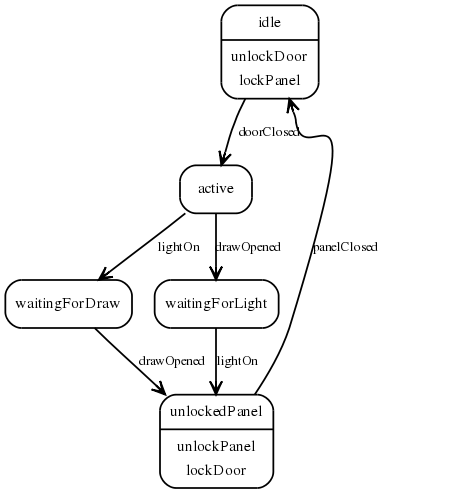
\includegraphics[scale=.7]{smgraph.png}
	\caption{Графическая нотация для языка StateMachine (из \cite{???})}\label{SM}
\end{figure}

В текстовой нотации автомат описывается с помощью ключевого слова \code{statemachine}, за которым следуем имя автомата и набор состояний в фигурных скобках. Пример использования текстовой нотации приведен в \lstref{SMText}. Cостояния описываются с помощью ключевого слова \code{state}; внутри состояния может находиться блок \code{do}, содержащий последовательность выходных воздействий, а также переходы, описываемые с помощью конструкции \code{on INPUT goto STATE}, где \code{INPUT} --- входное воздействие, а \code{STATE} --- состояние, в которое осуществляется переход.

Входные и выходные воздействия описываются вне блока \code{statemachine} с помощью ключевого слова \code{event}; каждое воздействие имеет уникальное имя и целочисленный код.

\begin{lstlisting}[label=SMText,float=htbp,caption=Текстовая нотация языка StateMachine]
event lockDoor 0; event unlockDoor 1;
event lockPanel 2; event unlockPanel 3;
event doorClosed 4; event doorOpened 5;
event lightOn 6; event drawOpened 7;
event panelClosed 8;

statemachine SecretCompartment {
	state idle {
		do {
			unlockDoor;
			lockPanel;
		}
		on doorClosed goto active;
	}
	state active {
		on lightOn goto waitingForDraw;
		on drawOpened goto waitingForLight;
	}
	state waitingForDraw {
		on drawOpened goto unlockedPanel;
	}
	state waitingForLight {
		on lightOn goto unlockedPanel;
	}
	state unlockedPanel {
		do {
			unlockPanel;
			lockDoor;
		}
		on panelClosed goto idle;
	}
}
\end{lstlisting}

Синтаксические правила языка StateMachine, выраженные в нотации \tool{Grammatic}, приведены в \lstref{SMGram}.

\begin{lstlisting}[xleftmargin=1cm,label=SMGram,caption=Грамматика языка StateMachine]
COMMENT : '//' [^'\n']*;
DIGIT : ['0'-'9'];
NAME_START : ['a'-'z''A'-'Z'_];
NAME_PART : NAME_START | DIGIT;
NAME : NAME_START NAME_PART*;
INT : DIGIT*;

system : event* stateMachine;
stateMachine : 'statemachine' NAME '{' state* '}';
state : 'state' NAME '{' do? (transition ';')* '}';
do : 'do' block;
transition : 'on' eventRef 'goto' stateRef;
stateRef : NAME;
block : '{' (commandRef ';')* '}';
eventRef : NAME;
comandRef : NAME;
event : 'event' NAME INT;
\end{lstlisting}

\chapter{Модули}

Поддержка модулей позволяет разработчику разделять спецификацию на несколько отдельных файлов и при необходимости использовать определения из одного файла повторно.  С точки зрения целевой мета-модели \tool{Grammatic}, модулю соответствует грамматика, определенная в отдельном файле. В данном разделе мы подробно опишем механизм работы таких модулей.

\section{Модули, цитирование и переименование}

Для описания модулей в \tool{Grammatic} не применяется никаких специальных синтаксических конструкций, поэтому файл, содержащий описание грамматики, уже является модулем. Для того, чтобы использовать один модуль внутри другого, применяется директива цитирования \tool{import}, синтаксис которого можно проиллюстрировать на следующем примере:
\begin{lstlisting}
import 'a/b/c/d.grammar' {A, B as C};

B : A C*;
\end{lstlisting} 
Директива \code{import} принимает два аргумента: идентификатор импортируемого файла в одинарных кавычках и список импортируемых символов в фигурных скобках. 

Идентификатором файла является его имя в \term{виртуальной файловой системе}, конфигурация которой подается на вход транслятору \tool{Grammatic} вместе с файлом основной грамматики. В простейшем случае (пустая конфигурация) виртуальная файловая система в точности соответствует физической, и идентификатором файла является просто путь на диске. Однако при использовании библиотек привязка к путям в физической файловой системе приводит к трудностям с переносимостью, поэтому виртуальная файловая система может предоставлять абстрактное представление физической, самостоятельно находя библиотечные модули. Подробнее формат описания виртуальной файловой системы разобран в Приложении \bad{???}.



\section{Атрибуты доступа}

в метаданных?
\section{Модульная грамматика для языка StateMachine}

Выделить описание событий/команд отдельно

\chapter{Шаблоны}

импортирование vs встраивание

Шаблон --- по сути функция, пример синтаксиса, результат

\section{Целевая мета-модель}
Чтобы их описать введем такие мета-классы

\section{Семантика шаблонов}
Алгоритм развертывания

\section{Статические гарантии корректности}
Система типов

Доказательство структурной корректности

\section{Примеры шаблонов выражений}

Как сделать последнюю ; необязательной

\section{Примеры параметризации модулей}

абстракция "Событие" и ее использование

\subsection{Параметризация грамматики выражениями}
\subsection{Параметризация грамматики другими грамматиками}

\chapter{Аспекты}

проблема дублирования грамматик и загрязнения кода аннотациями

(подсветка синтаксиса, форматирование...)

\section{Воплощение основных понятий AOP в \tool{Grammatic}}

Общая идея аспектов: точки встраивания, срезы, советы (модификации структуры + добавление метаданных)

Обосновать наличие незнания

\section{Квантификация и срезы}

язык срезов, семантика срезов

\section{Советы и семантика встраивания}

структура совета

семантика встраивания до, вместо, после

проблемы: 
	дважды нашли одно и то же (может быть, это вообще ошибка)
	переприсвоили атрибут --- ???
	
\section{Отделение метаданных с помощью аспектов}

Форматирование, синтаксис, СУТ

\section{Создание диалектов с помощью аспектов}

Сужение и расширение

\chapter{Выводы}

Возможности Grammatic

Наблюдения относительно автоматизации поддержки шаблонов и пр.



%%%%%%%%%%%%%%%%%%%%%%%%%%%%%%%%%%%%%%%%%%%%%%%%%%%%%%%%%%%%%%%%%%%%%%%%%%%%%
%%%%%%%%%%%%%%%%%%%%%%%%%%%%%%%%%%%%%%%%%%%%%%%%%%%%%%%%%%%%%%%%%%%%%%%%%%%%%
%% Неформальное описание

Основными понятиями языка Grammatic являются 

\section{Целевая мета-модель}

Спецификация на языке Grammatic описывает КС-грамматику (и, как мы покажем ниже некоторую дополнительную информацию, связанную с этой грамматикой). Грамматика (мета-класс Grammar) состоит из описаний символов (Symbol). Каждый символ имеет имя и набор продукций (Production), описывающих синтаксическую структуру этого символа. Телом продукции является грамматическое выражение (Expression).

Мета-класс Expression является абстрактным, а его конкретные потомки описывают различные типы выражений:
\begin{itemize}
\item Empty --- пустое выражение ($\varepsilon$);
\item SymbolReference --- ссылка на символ (соответствует вхождению символа в правой части продукции);
\item Sequence --- последовательность (конкатенация) выражений;
\item Alternative --- объединение (альтерация) выражений;
\item Iteration --- повторение (итерация) выражений, имеет атрибуты для верхней и нижней границ количества повторений;
\item LexicalDefinition --- лексическое определение, конкретные реализации:
	\begin{itemize}
		\item CharacterRange --- множество символов, задается как промежуток индексов кодовой таблицы Unicode;
		\item StringExpression --- строковый литерал, состоящий из символов Unicode;
		\item LexicalExpression --- ``лексические скобки'', выражение на которое ссылается экземпляр этого мета-класса не должно содержать ссылок на символы, определенные с помощью рекурсивных продукций.
	\end{itemize}
\end{itemize}


\section{Конкретный синтаксис}

Grammatic использует нотацию для языка EBNF, отличную от описанной в стандарте []. Эта нотация основана на используемой популярным генератором синтаксических анализаторов ANTLR [], которая объединяет средства описания лексических и синтаксических анализаторов, используя для тех и других операторы, применяемые для регулярных выражений.

Продукции, определяющие один и тот же символ группируются в \emph{синтаксические правила} вида:

\begin{lstlisting}
symbol
	: expression_1
	: expression_2
	...
	: expression_n
	;
\end{lstlisting}

Здесь expression_1, expression_2, \ldots, expression_n обозначают тела продукций, определяющих символ symbol. Нотация для грамматических выражений иллюстрируется следующим примером:
\begin{lstlisting}
example
	: #empty // Пустое выражение
	: a // Ссылка на символ a
	: a b // Последовательность 
	: a | b // Альтерация
	: a* // Итерация от 0 до бесконечности
	: a+ // Итерация от 1 до бесконечности
	: a? // Итерация от 0 до 1
	: ['a'--'z'] // Множество символов от 'a' до 'z'
	: 'abc' // Строка символов 'abc'
	: [[ a ]] // Лексические скобки
	: (a | b) c // Круглые скобки для группировки выражений
	;
\end{lstlisting}

В Листинге \ref{grammatic.grammar} приведена спецификация на языке Grammatic, описывающая нотацию самого языка Grammatic.

\begin{lstlisting}

...........

\end{lstlisting}

// примеры



\part{Генератор синтаксических анализаторов, построенный на базе \GRM{}}\label{part3}

\GRM{} предоставляет единый формат для записи контекстно-свободных грамматик и спецификаций на их основе. Если спецификация содержит дополнительную информацию, \GRM{} позволяет хранить ее в аннотациях. Как было показано выше, метаданные можно отделять от грамматики с помощью аспектов, получая несколько спецификаций из одной грамматики.

В настоящей главе мы рассмотрим генератор трансляторов \ATF{}, использующий возможности \GRM{} для решения задачи порождения кода транслятора сразу на нескольких языках программирования, причем гарантируется, что сгенерированный код не содержит ошибок типизации.

\chapter{Генераторы трансляторов}

Генератор трансляторов принимает на вход некоторую спецификацию и порождает код на некотором языке программирования, способный выполнять трансляцию текста во внутреннее представление в соответствии с правилами, указанными в спецификации.
Формат входных данных генератора мы будем называть \term{языком спецификации}, а язык программирования, код на котором генерируется --- \term{языком реализации}. Язык, синтаксис (и, возможно, семантику) которого описывает спецификация, мы будем называть \term{анализируемым языком}.

Языки спецификаций обычно основываются на атрибутных грамматиках \cite{???Knuth} в той или иной форме. В случае \ATF{} спецификация описывает схему синтаксически-управляемой трансляции \cite{???Dragon}, соответствующей \term{L-атрибутной грамматике} \cite{???}. Особенность таких грамматик состоит в том, что вне зависимости от направления анализа (нисходящий/восходящий) для вычисления атрибутов не требуется построения полного синтаксического дерева, поскольку атрибуты удается вычислять в процессе разбора. Наиболее популярные генераторы трансляторов используют именно этот подход \cite{???}.

\section{Модули анализа и генерации}

Любой генератор можно логически разделить на два взаимодействующих модуля: \term{модуль анализа}, читающий спецификацию, проверяющий ее корректность, и преобразующий ее во внутреннее представление, и \term{модуль генерации}, непосредственно порождающий код, читая внутреннее представление.
Модулей генерации может быть несколько, поскольку для переносимости реализации анализируемого языка и повторного использования спецификаций важно иметь возможность генерировать код на разных языках реализации.

// Рис?

Для удобства программиста важно выполнение следующего требования: \emph{если модуль анализа не обнаружил в спецификации ошибок и успешно построил внутреннее представление, модуль генерации должен построить код, не содержащий ошибок}.

В современных генераторах трансляторов это требование не соблюдается, что негативно сказывается на производительности разработчика. Проиллюстрируем это на примере разработки простого языка арифметических выражений с помощью одного из наиболее широкого используемых на сегодняшний день генераторов --- \tool{ANTLR}. Грамматика этого языка (без семантических действий) приведена в \lstref{arithexp}.
\begin{lstlisting}[texcl,language=ANTLR,label=arithexp,float=htbp,caption=Спецификация \tool{ANTLR} для языка арифметических выражений]
// Лексические правила
fragment LETTER : 'a'..'z' | 'A'..'Z' | '_' ;
fragment DIGIT  : '0'..'9' ;
VAR    : LETTER (LETTER | DIGIT)* ;
INT    : DIGIT+ ;
// Синтаксические правила
expr   : term (('+' | '-') term)* ;
term   : factor ('*' factor)* ;
factor : VAR | INT | '(' expr ')' ;
\end{lstlisting}
Нотация \tool{ANTLR} очень близка к нотации \GRM{} и в пояснении, по нашему мнению, не нуждается. Пусть необходимо разработать транслятор данного языка, вычисляющий значение выражения в процессе разбора. При этом значения переменных задаются внешней средой в виде объекта класса \code{Environment}, позволяющего получить значение переменной по имени. \tool{ANTLR} генерирует синтаксический анализатор основанный на методе рекурсивного спуска, поэтому каждое синтаксическое правило можно рассматривать как функцию, принимающую параметры (наследуемые атрибуты) и возвращающую значения (синтезируемые атрибуты). Семантические действия для правил \term{expr}, \term{term} и \term{factor} будут принимать объект \code{Environment} в качестве параметра и возвращать целочисленный результат вычисления. Соответствующий код на языке \tool{Java} пишется в фигурных скобках в том месте правила, где он должен быть вызван, аналогично схеме трансляции. 

Рассмотрим следующий вариант реализации семантических действий для правила \code{factor}:
\begin{lstlisting}[language=ANTLR]
factor[Environment env] returns [int result]
	: VAR { result = env.getValue($VAR.getText()); }
	| INT { result = $INT; }
	| '(' e=expr[env] ')' { result = e; } ;
\end{lstlisting}
По этой спецификации \tool{ANTLR} успешно генерирует код, содержащий следующий строки:
\begin{lstlisting}[language=Java,escapechar={!}]
	int result = 0;
	// ...
	Token INT2=null;
	// ...
	result = INT2;
\end{lstlisting}
При попытке скомпилировать этот фрагмент компилятором \tool{Java}, мы получим сообщение об ошибке на последней строке: значение \code{INT2} типа \code{Token} не может быть присвоено переменной \code{result}, имеющей тип \code{int}. Чтобы определить, в чем причина возникновения этой ошибки, нам необходимо вернуться к спецификации и вручную сопоставить сгенерированный код с соответствующим семантическим действием. В результате мы обнаружим, что использовали саму лексему \code{\$INT} вместо соответствующего ей текста, который можно получить, вызвав метод \code{getText()}. Мы вносим исправление в спецификацию:
\begin{lstlisting}[language=ANTLR]
factor //...
	| INT { result = $INT.getText(); }
\end{lstlisting}%$
Теперь нам необходимо снова запустить \tool{ANTLR}, чтобы получить и новую версию кода на \tool{Java}, а затем скомпилировать ее. Компилятор снова выдает сообщение об ошибке: значение \code{INT2.getText()} типа \code{String} не может быть присвоено переменной \code{result}, имеющей тип \code{int}. Мы снова возвращаемся к спецификации и конвертируем строку в число:
\begin{lstlisting}[language=ANTLR]
	| INT { result = Integer.parseInt($INT.getText()); }
\end{lstlisting}%$
После еще одного цикла генерации и компиляции, мы убеждаемся, что ошибка устранена. Всего нам понадобилось трижды запустить генератор и компилятор и дважды проследить, в каком месте в спецификации содержится причина возникновения ошибки в сгенерированном коде.

\section{Подходы, реализованные в современных генераторах}

В общем виде этот процесс, реализующийся при использовании любого генератора, не соответствующего сформулированному выше требованию, можно описать с помощью цикла, показанного на \figref{cycles} (а).
\begin{figure}[htbp]
\centering
\framebox{
\begin{minipage}{.45\textwidth}
\begin{enumerate}
\setlength{\itemsep}{0pt}
		\item Изменить спецификацию.
		\item Сгенерировать код.
		\item Попытаться скомпилировать код.
		\item Получить сообщения об ошибках в терминах языка реализации.
		\item Вручную отследить причины возникновения ошибок, содержащиеся в спецификации.
		\item Перейти к пункту 1.
\end{enumerate}
\centering
(а)
\end{minipage}
}
\framebox{
\begin{minipage}{.45\textwidth}
\begin{enumerate}
\setlength{\itemsep}{0pt}
		\item Изменить спецификацию.
		\item Попытаться сгенерировать код.
		\item Получить сообщения об ошибках в терминах языка спецификации.
		\item Перейти к пункту 1.
\end{enumerate}
\vspace{82pt}
\centering
(б)
\end{minipage}
}
\caption{Процесс устранения ошибки: (а) без статических проверок, (б) с проверками}\label{cycles}
\end{figure}
Основную сложность представляет необходимость вручную определять фрагмент спецификации, вызывающий ошибку. В принципе, модуль анализа мог бы делать это автоматически, но большинство современных инструментов, таких как \tool{ANTLR} или \tool{Bison} этого не делают, ограничиваясь лишь проверкой простейших условий, таких как наличие определений для всех символов, использованных в грамматике, без выполнения которых невозможно построение внутреннего представления. Семантические действия в этих инструментах рассматриваются как текстовые строки, и их содержание не анализируется.

Существуют генераторы, помогающие программисту в решении описанной проблемы. Так система \tool{Eli} \cite{???} анализирует сообщения об ошибках, выдаваемые компилятором, и автоматически находит соответствующие места в спецификации. Этот подход имеет два недостатка: во-первых, он привязан не только к одному языку реализации (используется язык \tool{C}), но и к одной версии компилятора, поскольку формат сообщений об ошибках может меняться. Система \tool{JastAdd} \cite{???} интегрируется с компилятором \tool{Java} и осуществляет точную диагностику ошибок, однако поддержка других языков реализации при таком подходе невозможна. Другой подход реализован в генераторе \tool{SableCC} \cite{???}: язык спецификаций вообще не поддерживает семантических действий, вместо этого разработчик должен вручную написать код на языке реализации, осуществляющий обход абстрактного синтаксического дерева и вычисляющий атрибуты. Такой подход в большей степени подвержен ошибкам и требует создания большего количества однотипного неинформативного кода.

\section{Задача \ATF{}}

Задачей \ATF{} является сокращение цикла работы со спецификацией до состояния, представленного на \figref{cycles} (б), при этом поддерживается возможность генерации кода на нескольких языках реализации по одной и той же спецификации.
Такая функциональность достигается за счет того, что семантические действия пишутся на абстрактном языке, в котором модуль анализа проверяет соблюдение правил типизации, а различные модули генерации строят код на соответствующих языках реализации.

В следующих разделах мы опишем язык спецификации, соответствующую систему типов и способы конфигурации модулей генерации и интеграции с различными языками реализации.

\chapter{Язык спецификаций \ATF{}}

\ATF{} использует нотацию \GRM{} для описания лексики и грамматики языков, при этом лексические правила явным образом помечаются атрибутом \code{lexical}, а игнорируемые терминалы, например, комментарии и пробельные символы --- еще и атрибутом \code{ignore}.

Спецификация описывает L-атрибутную трансляцию, при этом, аналогично \tool{ANTLR}, каждому правилу ставится в соответствие \term{функция трансляции}, принимающая наследуемые атрибуты в качестве параметров и возвращающая синтезируемые атрибуты. Это не означает, что \ATF{} способен генерировать только нисходящие анализаторы, использующие метод рекурсивного спуска, поскольку в случае восходящего анализа L-атрибутные определения тоже можно вычислить, вводя дополнительные продукции\footnote{Это делается автоматически в соответствующем модуле генерации.} \cite{???}. Тем не менее, о конструкциях, используемых в \ATF{}, удобнее всего думать в терминах рекурсивного спуска.

Телом функции трансляции, соответствующей правилу, является спецификация семантических действий, относящихся к различным позициям внутри правила, а также значения аргументов, передаваемых функциям трансляции, соответствующим символам, входящим в правые части продукций данного правила. В следующих подразделах мы опишем основные конструкции языка спецификации \ATF{} и проиллюстрируем их на примере интерпретатора арифметических выражений, который мы использовали в предыдущем разделе.

\section{Атрибуты и функции}

\term{Атрибут} в \ATF{} имеет имя и тип, в декларации разделяемые двоеточием, например
\begin{lstlisting}
result : Int
\end{lstlisting}
Атрибуты аналогичны переменным в императивных языках.

\term{Сигнатура} функции описывает ее имя, входные (наследуемые) и выходные (синтезируемые) атрибуты. Пример:
\begin{lstlisting}
factor (env : Environment) -> (result : Int)
\end{lstlisting}
Входные атрибуты описываются до стрелки, а выходные --- после. Отметим, что функция может возвращать кортеж из нескольких атрибутов.

В \ATF{} используются два вида функций:
\begin{itemize}
\item \term{функции трансляции} осуществляют разбор, обрабатывая входной поток, и вычисляют значения атрибутов;
\item \term{внешние функции} в \ATF{} описываются только сигнатурой, тела таких функций пишутся на языке реализации вне спецификации.
\end{itemize}
Встроенных операций, как и типов, в \ATF{} нет: арифметические и другие базовые операции реализуются в виде внешних функций.

Функции трансляции сопоставляются правилам грамматики следующим образом:
\begin{lstlisting}[language=Grammatic]
	N : ... ; // Синтаксическое правило
		translateN (in : Int) --> (out : Int) { // Сигнатура
			// Тело
		}
\end{lstlisting}
Полное описание функции, сигнатура и тело, записывается сразу после правила. Тело указывается в фигурных скобках. Одному правилу может соответствовать несколько функций трансляции, определяющих разные наборы семантических действий. 

В отличие от традиционной записи схемы трансляции, в \ATF{} семантические действия не встраиваются внутрь правил, а составляют тела функций трансляции. Для описания позиций, которым соответствуют действия, используются ключевые слова \code{after}, \code{before} и \code{at}. За счет этого удается достичь разделения семантических действий и правил грамматики.

Позиции семантических действий специфицируются следующим образом:
\begin{lstlisting}[escapeinside={!}{!},language=Grammatic]
	A : B C;
		translateA (...) --> (...) {
			...
			after B : !\textit{действие}! ;
			...
		}
\end{lstlisting}
После ключевого слова \code{after} указывается образец, \term{после} вхождения которого должно быть вычислено действие, отделенное двоеточием. В данном примере это просто вхождение символа \code{B}, но могут использоваться образцы произвольной сложности, описанные в предыдущей главе. Ключевое слово \code{before} имеет аналогичную семантику, но действие выполняется \term{до} вхождения, соответствующего образцу. 

Действия, указываемые справа от двоеточия, могут содержать декларации атрибутов, операции присваивания атрибутам и вызовы внешних функций. Если действие состоит из нескольких операций, они заключаются в фигурные скобки.

Ключевое слово \code{at} имеет иное значение: с его помощью описываются значения аргументов, передаваемых функциям трансляции и указывается, в какие атрибуты должны быть записаны результаты таких вызовов. После данного ключевого слова может быть указан только образец, имеющий тип \code{SymbolRefrence}. Пример:
\begin{lstlisting}[language=Grammatic]
	tmp : Int;
	at C : tmp = translateC(a, b) ;
\end{lstlisting}
В данном случае для обработки всех вхождений символа \code{C} будет вызвана функция трансляции \code{translateC} с аргументами \code{a} и \code{b}, а ее результат будет записан в \term{локальный} атрибут \code{tmp}. Локальный атрибут объявляется внутри тела функции трансляции и аналогичен локальной переменной.

\section{Пример спецификации}

Для того, чтобы проиллюстрировать использование основных конструкций, мы разберем спецификацию интерпретатора арифметических выражений, использующую эти конструкции. Для реализации интерпретатора нам понадобятся следующие внешние функции:
\begin{lstlisting}
	strToInt(s : String) --> (value : Int );
	value(env : Environment, variable : String) --> (value : Int);
	zero() --> (zero : Int);
	one() --> (one : Int);
	neg(x : Int) --> (negx : Int);
	add(x : Int, y : Int) --> (sum : Int);
	mul(x : Int, y : Int) --> (prod : Int);
\end{lstlisting}
Мы не имеем в виду никакого конкретного языка реализации. Все изложенное ниже имеет смысл для любого языка, поддерживающего числа и строки, в котором можно реализовать структуру данных, сопоставляющую строкам числа (для реализации среды).

Нам необходимо описать три функции трансляции --- по одной для каждого из нижеследующих правил:
\begin{lstlisting}
expr   : term (('+' | '-') term)* ;
term   : factor ('*' factor)* ;
factor : VAR | INT | '(' expr ')' ;
\end{lstlisting}
Каждая из этих функций будет принимать среду в качестве параметра и возвращать целочисленный результат. Для символа \code{factor} такая функция будет выглядеть так:
\begin{lstlisting}[
	label=factorTF,
%	caption=Функция трансляции для символа \code{factor},
	language=Grammatic]
factor : VAR | INT | '(' expr ')' ;           
  factor(Environment env) --> (Int result) { 
    after VAR : result = value(env, VAR#); // Внешняя функция
    after INT : result = strToInt(INT#);   // Внешняя функция
    at expr   : result = expr(env);        // Функция трансляции
  }
\end{lstlisting}
Использование ``\code{\#}'' после терминального символа (определение которого помечено атрибутом \code{lexical}) обозначает текстовое значение, сопоставленное данному соответствующее данному символу. Порядок следования элементов внутри функции не важен, поскольку каждое семантическое действие сопровождается информацией о позиции в правиле.

Приведенная в примере функция описывает следующие действия: 
\begin{itemize}
\item После обнаружения терминального символа \code{VAR} присвоить атрибуту \code{result} результат вызова внешней функции \code{value} от среды \code{env} и текста, соответствующего терминальному символу. Данная функция должна возвращать значение переменной с данным именем.
\item Аналогично для символа \code{INT}.
\item Для распознавания символа \code{expr} вызвать функцию разбора \code{expr} и параметром \code{env} и присвоить результат атрибуту \code{result}.
\end{itemize}
В некоторых случаях вызовы функций разбора могут быть опущены, но в данном примере это невозможно, поскольку необходимо указать значение аргумента.

Правило для символа \code{term} отличается тем, что имеет два вхождения одного и того же символа \code{factor}, семантические действия для которых различны (действия по ключевому слову \code{at} совпадают):
\begin{lstlisting}[
	language=Grammatic,	
	label=termTF,
%	caption=Translation function for \texttt{term},float=htbp
]
term : $f1=factor ('*' $f2=factor)* ;         
	term(Environment env) --> (Int result) {  
		Int f; // Объявление локального атрибута
		at factor : f = factor(env);      // Для обоих вхождений
		after $f1 : result = f;              // Только для \$f1
		after $f2 : result = mul(result, f); // Только для \$f2
	}
\end{lstlisting}
Для того, чтобы различать вхождения, в данном примере используются переменные \footnote{Синтаксис аналогичен использованному в \GRM{}, поскольку для реализации \ATF{} используется механизм аспектов, реализованный в \GRM{}}. Это позволяет сопоставить первому вхождению (переменная \code{\$f1}) присваивание, а второму (переменная \code{\$f2}) --- умножение и присваивание. Отметим, что вызов функции \code{factor} общий для обоих вхождений.


\begin{lstlisting}[
	language=Grammatic,	
	label=exprTF,
%	caption=Translation function for \texttt{expr},float=htbp
	]
expr : $t1=term ( $sgn=('+' | '-') term)* ;         
	expr(Environment env) --> (Int result) {  
  		at     term : t = term(env);
		before $t1  : {
			result = zero();
			sign = one();
		}
		after  term : result = add(result, mul(sign, t));
		before $sgn : sign = one();
		after  '-'  : sign = neg(sign);
  }
\end{lstlisting}

\chapter{Контроль типов в семантических действиях}

Общие правила системы типов

декларативное описание абстрактной системы типов

описание генератора

\chapter{Реализация на основе \GRM{}}

\chapter{Применение предложенного подхода}

Grammatic на Java

\chapter{Выводы}
\part{Автоматизация разработки средств композиции в предметно-ориентированных языках}\label{part4}

// Обобщаем подход, использованный в Grammatic

\chapter{Описание исходного языка}

Описанный в следующих разделах метод базируется на способе описания языка, принятом в современных средствах разработки~\cite{xText}. Этот способ основан на сходстве контекстно-свободных грамматик и мета-моделей: нетерминальные символы соответствуют классам, а правые части продукций задают значения атрибутов и ссылок. Эта аналогия позволяет установить соответствие между целевой мета-моделью и грамматикой и сгенерировать соответствующий транслятор.

Прямое соответствие между грамматикой и мета-моделью не всегда возможно, поскольку грамматика (рассматриваемая как описание алгебраических типов \cite{?}) задает множество деревьев, а мета-модель --- множество графов. То есть только мета-модели, все ссылки --- агрегирующие могут быть гарантированно сопоставлены некоторой грамматике.

В современных инструментах предпринимаются попытки решить эту проблему, позволяя пользователю указывать, что те или иные конструкции языка являются ключами для поиска объектов. Примером служат имена переменных: транслятор использует их как ключи для поиска в таблице символов. В общем виде такой процесс трансляции состоит из двух этапов: разбор текста (построение дерева) и разрешение ссылок (замыкание циклов в дереве).
При этом удобно выделять отдельную мета-модель для описания древовидного представления. Таким образом, описание языка состоит из следующих элементов:
\begin{enumerate}
\item контекстно-свободная грамматика,
\item мета-модель для древовидного представления,
\item описание соответствия между грамматикой и древовидной мета-моделью,
\item целевая мета-модель (с перекрестными ссылками),
\item описание процедуры разрешения ссылок, преобразующих дерево в экземпляр целевой мета-модели,
\item семантика языка --- способ обработки экземпляра целевой мета-модели, например, интерпретатор или генератор кода.
\end{enumerate}

Обработку шаблонов и аспектов можно добавить сразу после построения дерева или после разрешения ссылок. В первом случае осуществляется композиция деревьев, а во втором --- композиция графов. Оба подхода имеют свои достоинства и недостатки, однако предложенный ниже метод работает для произвольных мета-моделей, и одинаково применим в обоих случаях.

%\chapter{Текстовая нотация для моделей}
Ниже нам понадобится записывать формализованные утверждения, вовлекающие мета-модели и их экземпляры. Для этого в данном разделе мы опишем нотацию, позволяющую описывать соответствующие понятия в виде текста, что удобно при записи правил вывода, например, при формализации систем типов.

\section{Элементы мета-моделей}

Для описания элементов мета-моделей в формулах мы будем использовать следующие обозначения:

\begin{itemize}
\item Класс описывается именем $C$ и списками суперклассов $S$, ссылок $R$ и атрибутов $A$: $\class{C}{S}{R}{A}$. Иногда удобно объединять атрибуты и ссылки в единый список структурных элементов~$F$: $\classf{C}{S}{F}$.
\item Атрибут или ссылка описываются именем и типом: $\attribute{x}{\tau}$ и ???, соответственно.
\end{itemize}
%
\newcommand{\type}[2]{#1\left(#2\right)}%
\newcommand{\valts}{\mathbf{val}}%
\newcommand{\valt}[1]{\type{\valts}{#1}}%
\newcommand{\refts}{\mathbf{ref}}%
\newcommand{\reft}[1]{\type{\refts}{#1}}%
%
Типы структурных элементов имеют следующий вид:
\begin{itemize}
\item \code{String}, \code{Integer}, \code{Boolean} или \code{Character} --- имя примитивного типа, используется только для атрибутов;
\item $\reft{C}$ --- неагрегирующая ссылка на класс $C$;
\item $\valt{C}$ --- агрегирующая ссылка на класс $C$;
\item $\tau^?$ --- ссылка может иметь значение $NULL$, атрибут может быть не указан;
\item $\tau^*$ --- коллекция может содержать ноль или более элементов;
\item $\tau^+$ --- коллекция может содержать один или более элементов.
\end{itemize}
%
\section{Элементы моделей}

\newcommand{\obj}[3]{#1@#2\left\{#3\right\}}%
\newcommand{\refv}[2]{\mathbf{ref}\; #1@#2}%
%
Нотация для элементов моделей несколько более сложна, поэтому мы сначала приводим ее компактное описание в виде контекстно-свободной грамматики в \lstref{modelGrammar}, а затем поясняем.

Общий вид обозначения для объекта таков: 
\[\obj{C}{id}{r_i = u_i, a_i = v_i},\]
 где $C$ --- класс данного объекта, $id$ --- его уникальный идентификатор\footnote{Согласно основополагающим принципам ООП, каждый объект обладает \term{идентичностью} (identity, см. \cite{Booch}).}, $r_i = u_i$ --- ссылки и их значения, а $a_i = v_i$ --- атрибуты и их значения. Как и в случае классов, часто бывает удобно объединять атрибуты и ссылки и писать $\obj{C}{id}{f_i = v_i}$.

\begin{lstlisting}[label=modelGrammar,float=htbp,caption={Грамматика, описывающая запись моделей в виде текста}]
object : NAME '@' INT '{' (NAME '=' value ';')* '}' ;
value : attrValue | refValue;
attrValue : INT | STRING | CHAR | 'true' | 'false' 
          | 'NULL' | enumValue;
enumValue : NAME '.' NAME;
refValue : object | ref | list | set | 'NULL';
ref	: 'ref' '(' NAME '@' INT ')';
list : <Collection '[', ']'> ;
set : <Collection '{', '}'> ;

template Collection<start, end> : Production+ {
	: <?start> <?end>
	: <?start>  <List object, ','> <?end>
	: <?end> <List ref, ','> <?end>
}
\end{lstlisting}

Значениями атрибутов могут быть литералы примитивных типов (числа, строки, символы, булевские значения) или перечислений.

Значениями ссылок могут быть либо объекты (в случае агрегирующих ссылок), либо ссылочные выражения вида $\refv{C}{id}$, указывающие класс и идентификатор объекта, на который делается ссылка. Также ссылки могут иметь множественные значения --- коллекции\footnote{В принципе, множественные значения могут иметь и атрибуты, но для дальнейшего обсуждения это не важно, и мы не будем это учитывать.}, которые могут быть упорядоченными (списки) и неупорядоченными (множества).

Шаблонные выражения в правой части правил для списков (\code{list}) и множеств (\code{set}) разворачиваются следующим образом:
\begin{lstlisting}
list
	: '[' ']'
	: '[' object (',' object)* ']'
	: '[' ref (',' ref)* ']'
	;
set
	: '{' '}'
	: '{' object (',' object)* '}'
	: '{' ref (',' ref)* '}'
	;
\end{lstlisting}
Важно отметить, что коллекция может одновременно хранить либо объекты, либо ссылочные выражения, но не те и другие сразу.

На объектах определено отношение структурной эквивалентности, обозначаемое $\cong$ и заданное правилами, приведенными на \figref{cong}.
%
\begin{figure}[htbp]
	\centering
$$
\infer[obj]{
	\obj{C}{id_1}{f_i = v_i} \cong \obj{C}{id_2}{f_i = u_i}
}{
	\forall i. \; v_i \cong u_i
}
$$
$$
\infer[ref]{
	\refv{C}{id_1} \cong \refv{C}{id_2}
}{
	id_1 = id_2
}
\quad
\infer[refl]{x \cong x}{}
$$
$$
\infer[elist]{[\,] \cong [\,]}{}
\quad
\infer[list]{
	[x_1,\ldots,x_n] \cong [y_1,\ldots,y_n]
}{
	\forall i \in [1:n]. \; x_i \cong y_i
}
$$
$$
\infer[eset]{\{\} \cong \{\}}{}
\quad
\infer[set]{
	\{x_1,\ldots,x_n\} \cong \{y_1,\ldots,y_n\}
}{
	\forall i :\; x_i \cong y_{\pi(i)}
}
$$
	\caption{Отношение структурной эквивалентности объектов}\label{cong}
\end{figure}
Два объекта связаны отношением $\cong$, если они являются точными копиями друг друга, то есть отличаются только идентификаторами. В правиле \rref{set} $\pi$ обозначает некоторую перестановку из $n$ элементов, которая необходима для того, чтобы выразить неупорядоченность коллекции.
Очевидно, что $\cong$ является отношением эквивалентности.

\section{Структурные ограничения в виде системы типов}

\newcommand{\fromMM}{\MM{M} \Vdash}
Мета-модель накладывает ограничения на структуру объектов через типы и кратность ссылок и атрибутов. Эти ограничения мы записываем в виде системы типов, которая связывает мета-модель и объект отношением $\Vdash$. Запись $\fromMM x : \tau$ следует читать как ``\term{объект $x$ удовлетворяет ограничениям мета-модели $\MM{M}$ и имеет тип $\tau$}''.

Правила указанной системы типов приведены на \figref{TypesMM}. В этих правилах используется отношение ``подтип'', обозначаемое следующим образом:
$$
	\mbox{подтип} \subtype \mbox{супертип}.
$$
Это отношение является транзитивным рефлексивным замыканием минимального отношения, удовлетворяющего следующему требованию: $\classf{C}{\{S_i\}}{\_} \subtype S_i$.

\begin{figure}[htbp]
	\centering
$$
	\infer[object]{
		\fromMM \obj{C}{id}{f_i = v_i} : \valt{C}
	}{
		\classf{C}{\_}{f_i : \tau_i} \in \MM{M}&
		\fromMM v_i : \tau_i
	}
$$
$$
\infer[ref]{
	\fromMM \refv{C}{id} : C
}{}
\quad
\infer[null]{
	\fromMM NULL : \tau^?
}{}
$$
$$
\infer[elist]{
	\fromMM [\,] : \tau^*
}{}
\quad
\infer[list]{
	\fromMM [x_1, \ldots, x_n] : \type{TO}{\tau}^+
}{
	\forall i\in[1:n]. \; \fromMM x_i : \type{TO}{\tau} &
	TO \in \{\valts,\, \refts\}
}
$$
$$
\infer[eset]{
	\fromMM \{\} : \tau^*
}{}
\quad
\infer[set]{
	\fromMM \{x_1, \ldots, x_n\} : \type{TO}{\tau}^+
}{
	\forall i\in[1:n]. \; \fromMM x_i : \type{TO}{\tau} &
	TO \in \{\valts,\, \refts\}
}
$$
$$
\infer[relax]{
	\fromMM x : \tau^?
}{
	\fromMM x : \tau
}
\quad
\infer[relax^+]{
	\fromMM x : \tau^*
}{
	\fromMM x : \tau^+
}
\quad
\infer[subtype]{
	\fromMM x : \sigma
}{
	\fromMM x : \tau &
	\tau \subtype \sigma
}
$$
$$
\infer[superclass]{
	\forall i \in [1:n].\; \type{TO}{C} \subtype \type{TO}{S_i}
}{
	\classf{C}{\{S_i, \ldots, S_n\}}{\_} \in \MM{M} &
	TO \in \{\valts,\, \refts\}
}
$$
$$
\infer[enum]{
	\forall i \in [1:n]. \; \fromMM T.L_i : T
}{
	\mathbf{enum}\;T\{L_1,\ldots,L_n\} \in \MM{M}
}
\quad
\infer[bool]{
	\fromMM b : \mathtt{Boolean}
}{
	b \in \{\mathbf{true}, \mathbf{false}\}
}
$$
$$
\infer[int]{\fromMM INT : \mathtt{Integer}}{}
\quad
\infer[str]{\fromMM STRING : \mathtt{String}}{}
$$
$$
\infer[char]{\fromMM CHAR : \mathtt{Char}}{}
$$
	\caption{Структурная корректность объектов}\label{TypesMM}
\end{figure}




\chapter{Автоматическое построение языков, поддерживающих типизированные макроопределения}

В настоящем разделе описан метод, позволяющий по описанию языка построить описание более богатого языка, поддерживающего композицию с помощью шаблонов (типизированных макроопределений). Мы будем называть такой пополненный язык \term{шаблонным языком}, построенным на базе исходного языка.

\section{Неформальное описание механизма композиции, основанного на шаблонах}

\begin{Note}[О терминологии]
В англоязычной литературе используется термин \term{macro} \cite{MacroML,Cpp,Nemerle}. 
В качестве русского перевода этого термина употребляется либо слово ``макрос'', являющееся в сущности сленговым и полученное транслитерацией множественного числа ``macros'', либо слово ``макроопределение'', соответствующее более узкому по смыслу термину ``macro definition''. 
Близкой по смыслу альтернативой является термин ``шаблон'' (англ. ``template''), используемый в языке 
\tool{C++} 
\cite{C++} 
и ряде других~\cite{HTMP,Velocity,UML}. 

Мы считаем термин ``macro'' более подходящим для наших целей, и будем, следуя традиции, использовать более формальный вариант его перевода --- \term{макроопределение}.
\end{Note}

\subsection{Макроопределения в языке \tool{C}}

Наиболее известными системами, использующими макроопределения, являются язык программирования \tool{LISP}~\cite{Lisp} и препроцессор языка \tool{C}~\cite{C, Cpp}. В обоих случаях макроопределения служат для обогащения языка новыми конструкциями, которые преобразуются в базовые конструкции языка во время компиляции\footnote{Понятие ``время компиляции'' в данном контексте является собирательным и противопоставляется понятию ``время выполнения программы''.}, этот процесс называется \term{разворачиванием} макроопределений.

Приведем пример использования макроопределений в языке \tool{C}: пусть нам требуется реализовать односвязные списки. Для этого в первую очередь необходимо описать \emph{структуру} элемента списка, например, для списка целых чисел эта структура будет выглядеть следующим образом:
\begin{lstlisting}[language=C]
struct IntList {
	struct IntList* next;
	int data;
};
\end{lstlisting}
Для списка элементов другого типа, например, строк, структура будет очень похожей, но тип поля \code{data} будет отличаться:
\begin{lstlisting}[language=C]
struct StrList {
	struct StrList* next;
	char* data;
};
\end{lstlisting}
Дублировать описания для каждого нового типа элементов не очень удобно, поэтому мы напишем макроопределение, которое по данному типу элемента генерирует описание соответствующей структуры\footnote{Задача, которую мы решаем в этом примере с помощью макроопределений языка \tool{C}, более эффективно решается в языке \tool{C++} с помощью \emph{шаблонных структур}, которые можно рассматривать как узкоспециализированную разновидность макроопределений.}:
\begin{lstlisting}[language=C]
#define DEFLIST(name, type) struct name { \
	struct name *next; \
	type data; \
};
\end{lstlisting}
После директивы \code{\#define} следует \emph{имя} макроопределения, а за ним в скобках --- \emph{параметры}. Весь остальной текст --- это \emph{тело} макроопределения (знак ``$\backslash$'' используется для подавления перевода строки). Для того, чтобы использовать данное макроопределение, достаточно написать его имя и передать в скобках значения параметров (то есть \emph{аргументы}), например:

\begin{lstlisting}[language=C]
DEFLIST(StrList, char*)
\end{lstlisting}
В результате \emph{разворачивания} данного определения аргументы будут подставлены в тело вместо соответствующих параметров и мы получим определение структуры \code{StrList}, приводившееся выше. Аналогично можно получить определения структуры \code{IntList}, а также структуры элемента списка для любого типа. Заметим, что разворачивание происходит во время компиляции и результатом является исходный текст на языке \tool{C}, который, в свою очередь, транслируется в машинный код, причем транслятор ничего не знает о том, были использованы макроопределения или нет. 

Обобщая сведения, приведенные в данном примере, можно выделить следующие свойства, присущие механизму макроопределений\footnote{Такое обобщение имеет смысл, поскольку в различных языках и системах макроопределения функционируют схожим образом.}:
\begin{itemize}
\item Макроопределение состоит из \emph{списка параметров} и \emph{тела} и имеет уникальное \emph{имя}.
\item Тело макроопределения содержит конструкции на целевом языке (в нашем примере --- на языке \tool{C}) и ссылки на параметры. Также тело может содержать обращения к другим макроопределениям.
\item При разворачивании ссылки на параметры в теле макроопределения заменяются значениями соответствующих аргументов.
\item Разворачивание происходит во время компиляции программы.
\end{itemize}

Макроопределения представляют собой достаточно гибкий механизм повторного использования. В принципе, этот механизм не зависит от целевого языка, в который разворачиваются макроопределения. В частности, в языке \tool{C} поддержка макроопределений обеспечивается препроцессором \tool{Cpp} --- независимым программным средством, обрабатывающим исходный код \term{до} начала работы собственно компилятора языка \tool{C}. Препроцессор \tool{Cpp} может работать с любым текстом, не только с исходным кодом на языке \tool{C}, следовательно он (или аналогичный механизм) может применяться для повторного использования и в других языках, в частности в предметно-ориентированных, делая их более пригодными для использования в промышленных проектах.

Однако чисто текстовый препроцессор обладает одним важным недостатком: корректность результата разворачивания макроопределений никак не гарантируется, поскольку препроцессор манипулирует простым текстом и ``не знает'' о синтаксисе целевого языка.

Вернемся к примеру макроопределения, приведенному выше. Если программист допустит ошибку при использовании макроопределения \code{DEFLIST}, а именно перепутает порядок аргументов, что случается не так уж редко, препроцессор послушно выполнит свою работу:
\begin{lstlisting}[language=C]
DEFLIST(char*, StrList)
\end{lstlisting}
превратится в
\begin{lstlisting}[language=C]
struct char* {  // error: expected '\{' before 'char'
    struct char* *next; 
    StrList data; 
};
\end{lstlisting}
Получившийся код синтаксически некорректен, и компилятор, получив этот текст на вход, выдаст сообщение об ошибке:
\begin{lstlisting}[language=C]
DEFLIST(char*, StrList) // error: expected '\{' before 'char'
\end{lstlisting}
В итоге ошибка программиста обнаружена, но сообщение, выданное компилятором, записано в терминах программы, полученной после разворачивания макроопределений, и совсем не помогает программисту исправить ситуацию. Чтобы разобраться, в чем проблема, придется вручную рассмотреть код, полученный на выходе препроцессора, что является существенным затруднением при разработке больших проектов.
Описанная здесь проблема является основной причиной, по которой профессиональные программисты зачастую избегают широкого использования возможностей макроопределений в программах на \tool{C} \cite{CodeComplete}. 

Итак, чисто текстовый препроцессор позволяет легко обеспечить поддержку макроопределений в любом языке, но не обеспечивает своевременного обнаружения ошибок, что затрудняет разработку. В данной главе мы рассмотрим метод реализации макроопределений, который также пригоден для любого языка, но обеспечивает контроль корректности аргументов макроопределений с помощью специальной системы типов, что позволяет избежать проблем, присущих чисто текстовым препроцессорам. Такие макроопределения мы будем называть \emph{шаблонами} (templates).

\subsection{Шаблоны в языках, порожденных метамоделями}

Вернемся к примеру описания структуры элементов списка в языке \tool{C}. Для начала рассмотрим абстрактный синтаксис такого описания; соответствующая метамодель приведена на \figref{c-struct-mm}. 
%
\figdef{c-struct-mm}{Метамодель абстрактного синтаксиса описаний структур в языке \tool{C}}
%
Мы не ставим целью рассмотрение возможностей языка \tool{C} во всем их многообразии, поэтому наша метамодель позволяет оперировать лишь весьма ограниченным набором типов: структурами (\code{Struct} и \code{StructType}), указателями (\code{PointerType}) и примитивными типами \code{int} (\code{IntType}) и \code{char} (\code{CharType)}.

На \figref{int-list-struct} приведена диаграмма, соответствующая описанию структуры \code{IntList}, уже приводившемуся выше:
\begin{lstlisting}[language=C]
struct IntList {
	struct IntList* next;
	int data;
};
\end{lstlisting}
%
\figdef{int-list-struct}{Модель, описывающая структуру \code{IntList}}
%
Объект класса \code{Struct} хранит список, состоящий из объектов класса 	\code{Field}, каждый из которых имеет тип и имя.

Теперь преобразуем модель на \figref{int-list-struct} в шаблон, аналогичный макроопределению \code{DEFLIST} из предыдущего раздела:
\begin{lstlisting}[language=C]
#define DEFLIST(name, type) struct name { \
	struct name *next; \
	type data; \
};
\end{lstlisting}
Что для этого нужно сделать? Нужно добавить специальные объекты, представляющие структуру шаблона. На \figref{deflist-template} эти объекты выделены зеленым цветом фона.
%
\figdef{deflist-template}{Шаблон описания структуры элемента списка}
%
Рассмотрим новую диаграмму подробнее. Корневым элементом дерева встраивания является объект \code{DEFLIST} класса \code{Abstraction} --- это и есть шаблон, он содержит список \emph{параметров}, состоящий из двух объектов класса \code{Variable}, и \emph{тело} --- объект \code{struct}. Значение свойства \code{@name} объекта \code{struct} изменилось по сравнению с \figref{int-list-struct}: если раньше это была строка $\String{IntList}$, то теперь это объект класса \code{VariableUsage}, который ссылается на объект \code{name} класса \code{Variable}. Это соответствует использованию параметра теле шаблона. Аналогично изменилось из значение свойства \code{@type} объекта \code{data}: теперь это тоже объект класса \code{VariableUsage}, ссылающийся на параметр \code{type}.

Процедура разворачивания просто заменяет объекты \code{VariableUsage} в теле шаблона значениями соответствующих аргументов и получается модель, не содержащая ``шаблонных''объектов (зеленого цвета). Чтобы придать параметрам значения, требуется \code{применить} шаблон к соответствующим аргументам. 
%
\figdef{deflist-application-intlinst}{Применение шаблона}
%
На \figref{deflist-application-intlinst} приведена диаграмма, соответствующая применению шаблона \code{DEFLIST}, определенного выше, к аргументам $\String{IntList}$ и $\Object{}{\Ref{\String{IntType}}}{}$. Объект класса \code{Application} (\emph{применение}) содержит ссылку на применяемый шаблон и список аргументов. Соответствие между параметрами шаблона и аргументами устанавливается с помощью индексов в списках: нулевой аргумент соответствует нулевому параметру, первый --- первому и т.д. На рисунке параметры шаблона соединены с соответствующими аргументами пунктирными линиями. 

Заметим, что результатом разворачивания применения шаблона на \figref{deflist-application-intlinst} будет в точности модель на \figref{int-list-struct}, аналогично тому как разворачивание применения макроопределения
\begin{lstlisting}[language=C]
DEFLIST(IntList, int)
\end{lstlisting}
дает описание структуры \code{IntList}.

Заметим также, что аргументами шаблона в принципе могут быть и ``шаблонные'' объекты. 
%
\figdef{deflist-application-list-of-lists}{Использование применения шаблона в аргументах}
%
Так на \figref{deflist-application-list-of-lists} показано применения шаблона \code{DEFLIST} к списку аргументов, один из которых, в свою очередь, тоже является применением шаблона \code{DEFLIST}. В результате разворачивания шаблонов в этом примере получится описание структуры $\String{ListList}$ элементов списка, состоящего из списков целых чисел.

\subsection{Структура шаблонного языка}

Чтобы облегчить понимание, мы позволили себе некоторую вольность, приводя модельные термы с шаблонами на диаграммах в предыдущем разделе. Рассмотрим, например, \figref{deflist-template}: объекты \code{struct} и \code{data}, изображенные на этом рисунке, не удовлетворяют требованиям метамодели, приведенной на \figref{c-struct-mm}, поскольку эта метамодель определяет свойство \code{name} класса \code{Struct} как строковое, а на нашей диаграмме оно хранит объект класса \code{VariableUsage}; аналогично для свойства \code{type} объекта \code{data}. 

Такое положение вещей неудивительно: язык, порожденный метамоделью на \figref{c-struct-mm}, не поддерживает шаблоны, а для того, чтобы добавить в язык поддержку нового механизма, нужно как минимум пополнить его новыми конструкциями. Сделать это простым расширением метамодели (т.е. добавлением новых классов) затруднительно (подробнее по этому поводу см. Раздел \ref{mm-extension-vs-transformation}, поэтому мы построим новую метамодель, которая допускает использование шаблонных конструкций наравне с конструкциями исходного языка: см. \figref{c-struct-template-mm}.

\figdef{c-struct-template-mm}{Упрощенная метамодель пополненного языка описания структур}
%
Определению шаблона соответствует класс \code{Abstraction}, объекты которого содержат \emph{тело} (\code{body}) и список \emph{параметров} (\code{parameters}). Телом шаблона может являться любой модельный терм, так как свойство \code{body} имеет тип $\AnyT$. Абстрактный класс \code{Term}, занимающий центральное место на рисунке, с \emph{шаблонного терма}, то есть конструкции, к которой применима операция разворачивания. Уже знакомые нам классы \code{Application} и \code{VariableUsage} являются его подклассами.
Кроме того, из рисунка видно, что каждый класс исходной метамодели (\figref{c-struct-mm}) теперь является подклассом класса \code{Term}, и все свойства также имеют значения типа $\RefT{\String{Term}}$ или $\ClassT{\String{Term}}$. Это позволяет в качестве значения любого свойства использовать как конструкции исходного языка (теперь являющиеся шаблонными термами), так и ``чисто-шаблонные'' термы, то есть применения шаблонов и ссылки на параметры.

\subsection{Процесс разработки языка шаблонов}

В последующих разделах мы опишем метод, позволяющий пополнять языки автоматически. Процесс разработки языка с поддержкой шаблонов на основе уже существующего языка схематически представлен на \figref{macro-workflows}.
%
\figdef{macro-workflows}{Разработка и использование языков с поддержкой шаблонов}
%
Метамодель и интерпретирующая семантика языка \emph{Language} разрабатывается архитектором, после чего к метамодели применяется автоматизированная процедура трансформации, которую мы опишем ниже, в результате чего получается новая метамодель, поддерживающая шаблоны. Пользователь создает программу, удовлетворяющую требованиям пополненной метамодели, в своей программе он может использовать шаблоны. К этой программе применяется процедура разворачивания шаблонов, включающая в себя проверку типов аргументов (эту процедуру мы также опишем ниже). В результате получается программа, удовлетворяющая исходной метамодели языка \emph{Language}, к которой применима интерпретирующая семантика, разработанная архитектором. Таким образом, интерпретирующая семантика пополненного языка \emph{T-Language} получается автоматически как композиция процедуры разворачивания и интерпретирующей семантики исходного языка.

\section{Построение синтаксиса языка шаблонов}

Пусть даны метамодель $\M$ и интерпретирующая семантика $\Sem$ исходного языка, не поддерживающего шаблоны. Для того, чтобы ввести шаблоны в синтаксис этого языка, необходимо построить метамодель $\TM$, поддерживающую соответствующие конструкции. Кроме того, необходимо определить процедуру разворачивания шаблонов $\InstSign : \Language{\TM} \rightarrow \Language{\M}$, так, чтобы интерпретирующая семантика расширенного языка представляла собой композицию $\Sem \circ \InstSign$. В этом разделе мы рассмотрим процедуру построения метамодели $\TM$.

Как отмечалось выше, все языки шаблонов имеют общий набор базовых конструкций, которые можно описать с помощью метамодели \emph{базового языка шаблонов}: см. \figref{template-metamodel-full}\footnote{На этой диаграмме используется класс \code{Type}, который определен в метаметамодели $\MMM$, на \figref{types}.
}. 
%
\figdef{template-metamodel-full}{Полная метамодель базового языка шаблонов}
%
Основные классы этой метамодели были рассмотрены выше: базовый класс для всех шаблонных термов \code{Term}, определение шаблона (\code{Abstraction}), применение шаблона (\code{Application}) и использование шаблонного параметра (\code{VariableUsage}). Однако для полноценного функционирования языка шаблонов нам понадобятся некоторые дополнительные конструкции, специфичные для шаблонов в языках, порожденных метамоделями, в частности, класс \code{Inline}, позволяющий ``склеивать'' несколько коллекций (списков или множеств) в одну. Ниже мы опишем семантику шаблонных конструкций формально, а пока сосредоточимся на синтаксисе.

Чтобы получить метамодель $\TM$, необходимо к набору классов на \figref{template-metamodel-full} добавить классы, построенные по метамодели $\M$ и соответствующие конструкциям исходного языка (см. \figref{c-struct-template-mm}). Эти классы строятся функцией $\TC{\bullet}$, описанной на \figref{TC}.
%
\begin{figure}[htbp]
	\centering
\fbox{\parbox{.9\textwidth}{
	\centering
Преобразование классов и свойств:
$\TC{\Class{c}{S}{P}} = \Class{c^\mathcal{T}}
			{\Ref{\String{Term}}}{\TP{A}}$
			
$\TP{p : \tau} = p : \TT{\tau}$

Преобразование примитивных типов:
$
\TT{\CharT} = \CharT
\quad
\TT{\StringT} = \StringT
$

$
\TT{\IntegerT} = \IntegerT
\quad
\TT{\BooleanT} = \BooleanT
$

Преобразование коллекций и типов, допускающих $\Null$:

$\TT{\NullableT{\tau}} = \NullableT{\TT{\tau}}$

$
\TT{\SetT{\tau^+}} = \SetT{\TT{\tau}^+}
\qquad
\TT{\SetT{\tau^*}} = \SetT{\TT{\tau}^*}
$

$
\TT{\ListT{\tau^+}} = \ListT{\TT{\tau}^+}
\qquad
\TT{\ListT{\tau^*}} = \ListT{\TT{\tau}^*}
$

Преобразование типов, основанных на классах и перечислениях:

$
\TT{\ClassT{c}} = \ClassT{\TC{c}}
\qquad
\TT{\RefT{c}} = \RefT{\TC{c}}
$

$
\TT{\EnumT{e}} = \EnumT{e}
$

Преобразование типа $\AnyT$:

$\TT{\AnyT} = \AnyT$
}}
	\caption{Преобразование конструкций языка в шаблонные выражения}\label{TC}
\end{figure}

Вспомогательные функции $\TP{\bullet}$ и $\TT{\bullet}$ служат для преобразования свойств и типов, соответственно. В итоге, каждому классу исходной метамодели $\M$ сопоставляется класс-наследник класса \code{Term}, таким образом конструкции исходного языка становятся шаблонными термами. При этом ссылки также перенаправляются на класс \code{Term}, поскольку их значениями вместо конкретных объектов теперь могут выступать шаблонные термы (см. \figref{c-struct-template-mm}).

\section{Семантика языка шаблонов}

Как уже говорилось выше, семантика языка шаблонов задается операцией \term{разворачивания} $\InstSign : \Language{\TM} \rightarrow \Language{\M}$. Для того, чтобы построить $\InstSign$, нам потребуется несколько вспомогательных функций. И главная из них --- $\Inst{\gamma}{\bullet}$, где $r$ называется множеством \emph{внутренних ссылок}, а $\gamma$ -- \emph{средой}.

Отметим два свойства разворачивания, важных с технической точки зрения. Первое свойство состоит в том, что объекты, составляющие тело шаблона, при разворачивании \emph{копируются}, то есть создаются объекты с той же структурой, но другими идентификаторами. Это необходимо, например, для того, чтобы имели смысл шаблоны, использующие один и тот же параметр несколько раз. Рассмотрим, например, шаблон структуры, аналогичный следующему макроопределению:
\begin{lstlisting}[language=C]
#define PAIR(type) struct { type a; type b;}
\end{lstlisting}
%
\figdef{pair-template}{Шаблон $\String{PAIR}$ и его применение}
%
Соответствующий шаблон и его применение приведены на \figref{pair-template}. Результатом разворачивания шаблона должна быть структура, имеющая два поля одного и того же типа. Таким образом, объект, переданный в качестве аргумента при применении шаблона, должен встретиться дважды (свойство \code{type} встраивается в класс \code{Field}, поэтому использование двух ссылок на один и тот же объект невозможно), что будет являться нарушением определения модели, если идентификаторы двух объектов будут совпадать: если в модели будут ссылки на один из этих объектов, не будет возможности определить, на какой именно. Другой пример --- использование одного и того же шаблона несколько раз: см. \figref{deflist-application-list-of-lists}. Элементы тела шаблона должны быть скопированы, чтобы получился правильный результат.

Второе свойство состоит в том, что при копировании различаются \emph{внешние} и \emph{внутренние} ссылки.
\begin{Def}[Внутренние ссылки]
Пусть дан модельный терм $t$. Множество 
$$
r_t \eqdef \left\{ \Ref{id} \Or id \in \mathbf{dom}(\RContext_t) \right\}
$$
называется множеством \emph{внутренних ссылок} для терма $t$.
\end{Def}
Приведем пример: пусть 
$t = \List{1, \Object{\String{id}}{\RefSt{c}}{\RefSt{p} = \RefSt{id}}}$; в этом терме ссылка $\RefSt{id}$ является внутренней, поскольку объект, на который она ссылается является подтермом $t$ и, следовательно, $\String{id}$ принадлежит области значений контекста $\RContext_t$. Ссылка $\RefSt{c}$, напротив, внутренней не является, поскольку объект с идетификатором $\String{c}$ в терме $t$ не встречается.

При разворачивании шаблонов необходимо знать, какие ссылки являются внутренними для тела шаблона и его аргументов: только эти ссылки необходимо преобразовывать при разворачивании. Ссылки, не являющиеся внутренними, функция $\InstSign$ оставляет без изменений.

Для того, чтобы выбирать новые идентификаторы для объектов (это всегда возможно, потому что множество потенциальных идентификаторов бесконечно, а модели конечны), используем следующий прием: зафиксируем семейство биекций $\idmap_n : \ModelTerm \rightarrow \ModelTerm$, такое, что все идентификаторы, которые возвращают $\idmap_n$ не встречаются ни в одной из рассматриваемых моделей, причем множества значений различных $\idmap_n$ не пересекаются. Эти функции обеспечат согласованное копирование объектов и ссылок.

Введем специальное семейство функций для преобразования идентификаторов:
$$\idmap_{r,i}(id) = \left\{
	\begin{array}{ll}
		\newid_i(id), & id \in r\\
		id, & \mbox{в остальных случаях,}
	\end{array}\right.
$$
Здесь функция $\newid_i(x)$ --- это биекция, которая возвращает уникальный идентификатор, соответствующий $x$, и не совпадающий ни с одним другим идентификатором, использованным где-либо в разворачиваемой программе или возвращаемым какой-либо функцией $\newid_k$, где $k \neq i$, формально:
\begin{enumerate}
\item $\forall i.\;\newid_i(x) \MCong \newid_i(y) \leftrightarrow x \MCong y$;
\item $\forall i.\; \range(\newid_i) \cap ID = \emptyset$, где $\range(f)$ --- множество значений функции $f$, а $ID$ --- множество всех идентификаторов, встречающихся во входном шаблоне;
\item $\forall i \neq k.\; \range(\newid_i) \cap \range(\newid_k) = \emptyset$
\end{enumerate}
Ниже нам потребуется при каждом применении шаблона выбирать новую функцию $\newid_k$, такую, что она не была выбрана ни при каком другом применении шаблона. Мы будем обозначать индекс такой ``свежей'' функции символом ``$*$'', и, соответственно, писать, например, $\newid_*$.

На функциях преобразования идентификаторов определена операция последовательной композиции ``$\idmapcompose$'':
$$
  (\idmap_{r, n} \idmapcompose \idmap_{s, m})(id) = \left\{
	\begin{array}{ll}
		\newid_n(id), & id \in r\\
		\newid_m(id), & id \in s \setminus r\\
		id, & \mbox{в остальных случаях.}
	\end{array}\right.
$$

\begin{Def}[Среда]
Множество $\gamma$ пар вида вида $v = t$, где $v$~--- ссылка на переменную (объект класса \code{Variable}), а $t$ --- шаблонный терм.
\end{Def}
Среда ``запоминает'' значения, приданные параметрам при применении шаблона.

Приступим к определению функции $\Inst{\gamma}{\bullet}$. Сначала рассмотрим ее действие на применение шаблона:
{\small
$$
\trule{
	\Object{abs}{\RefSt{Abstraction}}{
		\begin{array}{rcl}
			\RefSt{body} &=& b,\\
			\RefSt{parameters} &=& \List{v_1, \ldots, v_n}\\
		\end{array}	
	}
}{
	\Inst{\gamma}{
		\Object{app}{\RefSt{Application}}{
			\begin{array}{rcl}
				\RefSt{abstraction} &=& \Ref{abs},\\
				\RefSt{arguments} &=& \List{a_1, \ldots, a_n}
			\end{array}	
		}
	} = \InstC{m'}{\gamma \cup \gamma'}{b}
}{app-inst}
$$}
Где $$\gamma' = \bigcup\limits_{i=1}^{n} \{ v_i = e_i \}, \qquad e_i = 
\InstC{m_i}{\gamma}{a_i}, \qquad m_i = \idmap_{r_{a_i}, *} \idmapcompose m,
$$
$$m' = \idmap_{r', *} \idmapcompose m, \qquad
r' = r_b \cup \bigcup\limits_{1}^{n} r_{e_i}.$$

Это правило описывает работу процедуры разворачивания шаблонов в случае применения шаблона, описание которого приведено над горизонтальной чертой: тело шаблона обозначено метапеременной $b$, а параметры --- метапеременными $v_i$. Выражение под горизонтальной чертой означает, что при разворачивании применения такого шаблона, в случае если переданы аргументы $a_i$, число которых в точности совпадает с числом параметров шаблона, результатом является $\InstC{m'}{\gamma \cup \gamma'}{b}$, то есть результат разворачивания тела шаблона $b$ в пополненной среде $\gamma'$, содержащей новые значения для параметров $v_i$, и в контексте функции $m'$, учитывающей внутренние ссылки тела и аргументов. Заметим, что передача параметров происходит \emph{по значению}: в среде $\gamma'$ переменным $v_i$ сопоставляются не аргументы $a_i$, а результаты их разворачивания. Кроме того, заметим, что в случае передачи неверного числа аргументов поведение не определено.

Далее рассмотрим действие процедуры разворачивания на использование переменной:
$$
\trule{
	\{v = t\} \subseteq \gamma
}{
	\Inst{\gamma}{\Object{u}{\RefSt{VariableUsage}}{\RefSt{variable} = \Ref{v}}} = \Copy{t}
}{var-inst}
$$ 
Предсказуемым образом, результат берется из среды $\gamma$, и поведение определено только в том случае, если среда содержит значение для данной переменной. Результатом разворачивания является \emph{копия} терма, содержащегося в среде, чтобы обеспечивается использованием функции $\Copy{\bullet}$, определяемая следующим образом:

$$
\Copy{t} = \left\{
	\begin{array}{ll}
		\multicolumn{2}{l}{		
			\Object{m(id)}{c}{p_1 = \Copy{v_1}, \ldots, p_n = \Copy{v_n}},
		} \\
		\multicolumn{2}{l}{			
			\qquad \qquad \qquad t = \Object{id}{c}{p_1 = v_1, \ldots, p_n = v_n}
		}\\
		\Ref{m(id)}\\%, & t = \Ref{id},\; id \in r\\
		\List{\Copy{x_1}, \ldots, \Copy{x_n}}, & t = \List{x_1, \ldots, x_n}\\
		\Set{\Copy{x_1}, \ldots, \Copy{x_n}}, & t = \Set{x_1, \ldots, x_n}\\
		t, & \mbox{в остальных случаях}
	\end{array}
\right.
$$
Заметим, что  внутренние ссылки при копировании перенаправляются на копии объектов.

Перейдем к правилам разворачивания для классов, порожденных преобразованием $\TC{\bullet}$. Строго говоря, соответствующих правил должно быть столько же, сколько и самих этих классов, и правило для класса $C$ выглядит следующим образом:
$$
\trule{
	C = \Class{c}{S}{\ldots} &
	t = \Object{id}{c^\mathcal{T}}{p_i = v_i}
}{
	\Inst{\gamma}{t} = \Object{m(id)}{c}{p_i = \Inst{\gamma}{v_i}}
}{ds-inst(С)}
$$ 
Процедура разворачивания применяется к значениям всех свойств объекта класса $c^\mathcal{T} \eqdef \TC{C}$.

Объекты классов, не являющихся результатом преобразования $\TC{\bullet}$, не изменяются при разворачивании. На практике это касается, в первую очередь, перечислений (enumerations).

При разворачивании ссылки транслируются с помощью функции $m$:
$$
\trule{
%	\Inst{\gamma}{\Object{id}{c}{\ldots}} = \Object{id'}{c'}{\ldots}
}{
	\Inst{\gamma}{\Ref{id}} = \Ref{m(id)}
}{inner-ref-inst}
$$ 
То есть внутренние ссылки после разворачивания меняют идентификатор, поскольку новая ссылка должна показывать на новый объект. 
Это необходимо для того, чтобы, например, при разворачивании шаблона на \figref{deflist-template} ссылки, находящиеся внутри тела шаблона, указывали на объекты, созданные при разворачивании.
Ссылки, не являющиеся внутренними, идентификаторы не меняют.

Перейдем к разворачиванию списков. Здесь важную роль играет конструкция \code{Inline}, позволяющая ``склеивать'' несколько коллекций в одну. При $n \ge 0$
$$
\Inst{\gamma}{\List{x_1, \ldots, x_n}} = \InstL{\gamma}{x_1} \LConcat \ldots \LConcat \InstL{\gamma}{x_n},
$$ 
где $\LConcat$ --- операция конкатенации списков. Таким образом, действие функции $\Inst{\gamma}{\bullet}$ сводится к конкатенации результатов действия вспомогательной функции $\InstL{\gamma}{\bullet} : \Language{\TM} \rightarrow \ListT{\Language{\TM}}$ на элементы списка. Сама функция $\InstL{\gamma}{\bullet}$ определяется следующим образом:
$$
\trule{
\Inst{\gamma}{t} = \List{x_1, \ldots, x_n}
}{
	\InstL{\gamma}{\Object{i}{\RefSt{Inline}}{\RefSt{subject} = t}} = \List{x_1, \ldots, x_n}
}{}
$$
В случае, если $t$ --- аргумент конструкции \code{Inline} --- разворачивается в список, этот список и является результатом; в противном случае результат ``заворачивается'' в дополнительный список:
$$
	\InstL{\gamma}{t} = \List{\Inst{\gamma}{t}}.
$$ 
Приведем пример:
\begin{align*}
	\Inst{\emptyset}{\List{1, \Object{i}{\RefSt{Inline}}{\RefSt{subject} = \List{3, 4}}}} = \\
=	\InstL{\emptyset}{1} \LConcat \InstL{\emptyset}{\Object{i}{\RefSt{Inline}}{\RefSt{subject} = \List{3, 4}}} = \\
=	\List{1} \LConcat \List{3, 4} = \\
=	\List{1, 3, 4}
\end{align*}

Для множеств правила аналогичные:
$$
\trule{
n \ge 0
}{
	\Inst{\gamma}{\Set{x_1, \ldots, x_n}} = \InstS{\gamma}{x_1} \cup \ldots \cup \InstS{\gamma}{x_n}
}{set-inst}
$$ 

$$
\trule{
\Inst{\gamma}{t} = \Set{x_1, \ldots, x_n}
}{
	\InstS{\gamma}{\Object{i}{\RefSt{Inline}}{\RefSt{subject} = t}} = \Set{x_1, \ldots, x_n}
}{}
$$ 

Осталось рассмотреть правила разворачивания для значений примитивных типов. Для $x \in \{\Null\} \cup  \Sigma^* \cup \mathbb{Z} \cup \mathbb{B}$
$$
	\Inst{\gamma}{x} = x.
$$

%\begin{Def}[Нормальная форма шаблонного терма]
%Шаблонный терм находится в \term{нормальной форме}, если он не содержит объектов классов \code{Application}, \code{VariableUsage} и \code{Inline} и ссылок на такие объекты.
%\end{Def}
%Другими словами, шаблонный терм в нормальной форме не нуждается в разворачивании: в нем нет шаблонных конструкций.

\section{Система типов}

!!!!!!!!!!!!! Шаблон --- это такой типизированный макрос, вот такой вот воображаемый шаблон мог бы нас спасти
\begin{lstlisting}[language=C]
#define DEFLIST(name : NAME, type : TYPE) : STRUCT = struct name { \
	struct name *next; \
	type data; \
};
\end{lstlisting}
Типовые аннотации позволят нам проконтролировать корректность в момент применения шаблона
\begin{lstlisting}[language=C]
DEFLIST(char*, StrList) // ошибка: первым аргументом должен быть тип
\end{lstlisting}
Для метамоделей это все означает, что мы хотим, чтобы типы гарантировали, что в результате получится экземпляр метамодели исходного языка.

Для того, чтобы гарантировать, что результат применения шаблона будет корректным с точки зрения целевой мета-модели, мы определяем систему типов для языка шаблонов. Типы указываются в базовых шаблонных конструкциях \code{Abstraction}  и \code{Variable} (см.~\figref{template-metamodel-full}), для этого используются классы из метаметамодели $\MMM$ (см.~\figref{types}). 

В этом разделе мы определим отношение \emph{типизируемости в контексте}: запись 
$$\Gamma \vdash x : \tau$$
читается как ``шаблонный терм $x$ имеет тип $\tau$ в контексте $\Gamma$'', где \emph{типовый контекст} $\Gamma$ является множеством пар $v : \rho$, где $v$ --- объект класса \code{Variable}, а $\rho$ --- тип. В случае, когда контекст пуст, слева от знака выводимости ничего не пишется: 
$$\vdash x : \tau.$$
Если одна и та же переменная встречается в типовом контексте дважды, такой контекст называется \emph{некорректным}, и в нем, по определению, никакой терм не имеет типа. Отметим, что, если $\vdash x : \tau$, то для любого корректного $\Gamma$ выполняется $\Gamma \vdash x : \tau$.

Ниже приводятся правила вывода, определяющие отношение выводимости. При этом используется язык типов из определения \ref{deftype}, пополненный специальными значениями для описания сигнатур шаблонов и результатов работы конструкции \code{Inline}, определенными ниже. 

Первое правило определяет требования к структуре объявления шаблона (класс \code{Abstraction}): если параметры $v_i$ имеют типы $\tau_i$, а тело в контексте, состоящем из пар $v_i : \tau_i$ имеет тип $\rho$, то соответствующий шаблон имеет тип $(\tau_1, \ldots, \tau_n) \rightarrow \rho$ в пустом контексте.
{\small
$$
\trule{
	v_i = \Object{id_i}{\RefSt{Variable}}{\RefSt{type} = \tau_i}, i \in [1..n], n \ge 0
	&
	\bigcup\limits_1^n \left\{ v_i : \tau_i \right\} \vdash b : \rho
}{
	\vdash \Object{abs}{\RefSt{Abstraction}}{
		\begin{array}{rcl}
			\RefSt{body} &=& b,\\
			\RefSt{parameters} &=& \List{v_1, \ldots, v_n},\\
			\RefSt{type} &=& \rho\\
		\end{array}	
	} : (\tau_1, \ldots, \tau_n) \rightarrow \rho
}{}
$$}
Запись $(\tau_1, \ldots, \tau_n) \rightarrow \rho$ можно читать как ``шаблон, принимающий параметры типов $\tau_i$ и возвращающий тип $\rho$''. Эта конструкция аналогична функциональным типам в $\lambda$-исчислении. Заметим, что шаблоны ``высших порядков'', то есть шаблоны, параметрами которых являются другие шаблоны, не поддерживаются, поскольку в языке типов, определенном \figref{types} эта конструкция не описана. ``Функциональные'' типы встречаются только как промежуточные результаты при проверке корректности шаблонов, и поэтому не требуют представления в виде модельных термов. Кроме того, заметим, что это правило запрещает рекурсивные определения шаблонов.

Следующее правило регулирует применение шаблонов: аргументы $a_i$ должны иметь типы, соответствующие типам параметров шаблона.
{\small
$$
\trule{
	\vdash \Object{abs}{\RefSt{Abstraction}}{\ldots
%		\begin{array}{rcl}
%			\RefSt{body} &=& b,\\
%			\RefSt{parameters} &=& \List{v_1, \ldots, v_n}\\
%		\end{array}	
	} : (\tau_1, \ldots, \tau_n) \rightarrow \rho
	&
	\Gamma \vdash a_i : \tau_i, i \in [1..n]
}{
	\Gamma \vdash
		\Object{app}{\RefSt{Application}}{
			\begin{array}{rcl}
				\RefSt{abstraction} &=& \Ref{abs},\\
				\RefSt{arguments} &=& \List{a_1, \ldots, a_n}
			\end{array}	
		}
	: \rho
}{}
$$}
Типом результата применения шаблона является $\rho$ --- тип возвращаемого значения, обсуждавшийся выше.

Использование переменной типизируется согласно контексту:
$$
\trule{
	\{v : \tau\} \subseteq \Gamma
}{
	\Gamma \vdash 
		\Object{u}{\RefSt{VariableUsage}}{\RefSt{variable} = \Ref{v}} : \tau
}{}
$$ 
В случае, если переменная в контексте $\Gamma$ не упоминается, ее использование не имеет типа.

Перейдем к правилам типизации объектов. Начнем с объектов классов, полученных в результате применения преобразования $\TC{\bullet}$. Пусть $C = \Class{c}{S}{p_i}, i \in [1..n]$, тогда
$$
\trule{
	p_i = \Object{id_i}{\RefSt{Property}}{\RefSt{type} = \tau_i} &
	\Gamma \vdash v_i : \tau_i
}{
	\Gamma \vdash \Object{id}{c^\mathcal{T}}{p_i = v_i} : \ClassT{c}
}{}
$$ 
То есть объект класса $\TC{C}$ типизируется классом $C$.
Ссылки, в свою очередь, типизируются в соответствии с тем, на что они указывают:
$$
\trule{
	\Gamma \vdash \Object{id}{k}{\ldots} : \ClassT{c} &
}{
	\Gamma \vdash \Ref{id} : \RefT{c}
}{}
$$ 

Разрешается неявное приведение типа к более широкому (согласно отношению ``$\subtype$''):
$$
\trule{
	\Gamma \vdash x : \tau &	
	\tau \subtype \rho	
}{
	 \Gamma \vdash x : \rho
}{}
$$ 

Приступим к описанию правил типизации для коллекций. Начнем со списков. Нам необходимо выразить несколько свойств процедуры разворачивания, наибольшие затруднения представляет конструкция \code{Inline}: если ее аргументом является список, то сама конструкция имеет место только внутри другого списка. Кроме того, нам необходимо следить за тем, чтобы тип $\ListT{\tau^+}$ приписывался только тем конструкциям, которые гарантированно разворачиваются в непустые списки (для множеств ситуация полностью аналогичная). Для решения этих проблем нам потребуются некоторые технические обозначения:
\begin{itemize}
\item $\LI{\tau}$ --- составляющие списка типа $\ListT{\tau^+}$, то есть непустого списка;
\item $\ELI{\tau}$ --- составляющие списка типа $\ListT{\tau^*}$, то есть, возможно, пустого списка.
\end{itemize}

При этом отношение ``$\subtype$'' работает следующим образом:
$$
\tau \subtype \LI{\tau},
\qquad
\LI{\tau} \subtype \ELI{\tau}.
$$
\noindent
Заметим, что, аналогично ``функциональным'' типам, данные типы никогда не используются в аннотациях к переменным или абстракциям: они возникают только как промежуточные результаты при проверке корректности шаблонных термов.

Итак, первое правило, типизирующее списки, выглядит так:
$$
\trule{
	\Gamma \vdash x_i : \ELI{\tau} & i \in [1..n] & n \ge 0
}{
	\Gamma \vdash \List{x_1, \ldots, x_n} : \ListT{\tau^*}
}{}
$$ 
Список состоящий из нуля или более элементов типа $\ELI{\tau}$ имеет тип $\ListT{\tau}$, то есть может быть пустым: во-первых, в нем может не быть ни одного элемента, а во-вторых, все его элементы могут быть развернуты функцией $\InstL{\gamma}{\bullet}$ в пустые списки. Чтобы список был непустым, он должен содержать хотя бы один элемент типа $\LI{\tau}$:
$$
\trule{
	\Gamma \vdash x_i : \ELI{\tau} & i \in [1..n] &
	\exists k. \Gamma \vdash x_k : \LI{\tau}
}{
	\Gamma \vdash \List{x_1, \ldots, x_n} : \ListT{\tau^+}
}{}
$$ 

Перейдем к правилам для конструкции \code{Inline}. Непустой список она преобразует в значение типа $\LI{\tau}$, поскольку такой шаблонный терм не может быть развернут в пустой список:
$$
\trule{
	\Gamma \vdash x : \List{\tau^+}
}{
	\Gamma \vdash \Object{id}{\RefSt{Inline}}{\RefSt{subject} = x} : \LI{\tau}
}{}
$$ 
\noindent 
Если список может быть пустым, получается значение типа $\ELI{\tau}$:
$$
\trule{
	\Gamma \vdash x : \List{\tau^*}
}{
	\Gamma \vdash \Object{id}{\RefSt{Inline}}{\RefSt{subject} = x} : \ELI{\tau}
}{}
$$ 
\noindent
Напомним, что $\tau \subtype \LI{\tau} \subtype \ELI{\tau}$ и, соответственно, терм не являющийся коллекцией, автоматически имеет тип элемента списка.

Для множеств все правила абсолютно аналогичны. Пусть
\begin{itemize}
\item $\SI{\tau}$ --- составляющие непустого множества;
\item $\ESI{\tau}$ --- составляющие, возможно, пустого множества.
\end{itemize}
При этом $\tau \subtype \SI{\tau} \subtype \ESI{\tau}$. Тогда правила выглядят следующим образом:

$$
\trule{
	\Gamma \vdash x_i : \ESI{\tau}, i \in [1..n], n \ge 0
}{
	\Gamma \vdash \Set{x_1, \ldots, x_n} : \SetT{\tau^*}
}{}
\qquad
\trule{
	\Gamma \vdash x_i : \ESI{\tau}, i \in [1..n] &
	\exists k. \Gamma \vdash x_k : \SI{\tau}
}{
	\Gamma \vdash \Set{x_1, \ldots, x_n} : \SetT{\tau^+}
}{}
$$ 
Для конструкции \code{Inline}:
$$
\trule{
	\Gamma \vdash x : \Set{\tau^+}
}{
	\Gamma \vdash \Object{id}{\RefSt{Inline}}{\RefSt{subject} = x} : \SI{\tau}
}{}
$$ $$
\trule{
	\Gamma \vdash x : \Set{\tau^*}
}{
	\Gamma \vdash \Object{id}{\RefSt{Inline}}{\RefSt{subject} = x} : \ESI{\tau}
}{}
$$ 

Нам осталось привести правила для $\Null$ и примитивных типов (а также перечислений). Итак, 
$$
\trule{
\mbox{Для любого } \tau
}{
	 \vdash \Null : \NullableT{\tau}
}{}
$$
К тому же всякий тип $\tau$ может быть расширен до $\NullableT{\tau}$, поскольку выше мы определяли $\tau \subtype \NullableT{\tau}$.

Примитивные типы при использовании с шаблонами, не изменяются. Для $\tau$ вида $\EnumT{e}$, $\CharT$, $\StringT$, $\IntegerT$, $\BooleanT$:
$$
\trule{
	x \in \denot{\tau} 
}{
	 \vdash x : \tau
}{}
$$ 

Чтобы показать, что ограничения, накладываемые системой типов адекватны требованиям мета-модели, докажем следующую лемму.
\begin{Lemm}[О нормальных формах]\label{LemmNF}
Если шаблонное выражение $e$ имеет нормальную форму и $\vdash e : \tau$, то $\fromMM \ct{e} : \tau$.
\end{Lemm}
\begin{proof}
Достаточно заметить, что в дереве вывода для $\vdash e : \tau$ правила \rref{var}, \rref{abstr}, \rref{appl}, \rref{item*} и \rref{item$^+$} не встречаются, а остальные правила в системе типов для шаблонов имеют прямые аналоги в системе требований мета-модели на \figref{TypesMM}.
\end{proof}

Дополнительно к правилам типизации, на язык шаблонов накладывается следующее требование: 
%\begin{enumerate}[(a)]
%\item 
\emph{Никакой шаблон не должен быть достижим из своего тела по ссылкам}. Это требование гарантирует отсутствие рекурсии в определениях шаблонов.
%\item \emph{Если множество использований некоторого параметра непусто, в нем должно содержаться хотя бы одно использование, на которое указывает агрегирующая ссылка.} Это требование гарантирует, что в результате разворачивания не возникнет объектов, не агрегируемых результирующей моделью.
%\end{enumerate}

\section{Структурная корректность}

Система типов накладывает ограничения на шаблоны. Шаблоны и шаблонные выражения, удовлетворяющие правилам типизации, при разворачивании порождают конечные объекты, удовлетворяющие требованиям целевой мета-модели.
Для того, чтобы убедиться в этом, покажем, что для системы типов и семанитки языка шаблонов выполняются свойства \term{сохранения типов} и \term{нормализации}~\cite{Pierce}. 

Как отмечалось выше, необходимым условием корректного поведения является тот факт, что функция разворачивания получает на вход выражение, в котором соблюдаются правила системы типов. Это условие формализовано в следующем определении.

\begin{Def}\label{agree}
Среда $\gamma$ называется \term{согласованной с контекстом} $\Gamma$, если все ее элементы имеют допустимые типы:
$$
	\forall p \, : \, 
		\{p = e\} \subseteq \gamma 
			\Rightarrow 
		\left\{\begin{array}{l}		
		\{p : \tau\} \subseteq \Gamma \\
		\Gamma \vdash e : \tau
		\end{array}\right.
$$
\end{Def}

Теперь докажем первое из упомянутых выше свойств.

\begin{Th}[О сохранении типов]\label{ThTP}
Если среда $\gamma$ согласована с контекстом $\Gamma$ и \mbox{$\Gamma \vdash e : \tau$}, то \mbox{$\Gamma \vdash \Inst{\gamma}{e} : \tau$}. Другими словами, преобразование $\Inst{}{\bullet}$ сохраняет типы.
\end{Th}
\begin{proof}
Будем вести индукцию по определению $\Inst{\gamma}{e}$.

\noindent\textbf{База.} Правило \rref{ds-inst(C)} сохраняет типы, поскольку из объекта класса $\TC{C}$ получается объект того же класса, а правило \rref{ds-type(C)} выводит тип из класса объекта.

\noindent\textbf{Переход.} 
В правиле \rref{app-inst} среда расширяется, и нам необходимо показать, что результат согласован с контекстом. Это обеспечивается требованиями к типам параметров, накладываемыми правилом \rref{appl} и способом формирования контекста в правиле \rref{abstr}. Из этого по предположению индукции следует, что правило \rref{app-inst} сохраняет типы.

Так же по предположению правило \rref{var-inst} сохраняет типы.
\end{proof}

Свойство нормализации формулируется следующим образом:

\begin{Th}[О нормализации]\label{ThNorm}
Если среда $\gamma = \cup \{p_i = e_i\}$ согласована с контекстом $\Gamma$, все $e_i$ имеют нормальную форму и $\Gamma \vdash e : \tau$, то результат вычисления $\Inst{\gamma}{e}$ имеет нормальную форму.
\end{Th}
\begin{proof} 
Будем вести индукцию по определению $\Inst{\gamma}[\bullet]$.\\
\textbf{База.} Результат применения правила \rref{var-inst} имеет нормальную форму, поскольку все элементы среды имеют нормальную форму.
\textbf{Переход.} В правиле \rref{app-inst} среда пополняется значениями, имеющими нормальную форму, поэтому по предположению индукции вызовы $\Inst{\gamma}{a_i}$ и $\Inst{\gamma \cup \gamma'}{b}$ заканчиваются за конечное число шагов и результат имеет нормальную форму.

Правило \rref{ds-inst(C)} заменяет значения ссылок результатами разворачивания, имеющими нормальную форму, следовательно и результат применения правила имеет нормальную форму.
\end{proof}

Требование о том, чтобы все элементы среды имели нормальную форму выполняется для пустой среды, следовательно теорема применима для разворачивания шаблонных выражений, применяемых на практике.

Мы показали, что функция $\Inst{}{\bullet}$ корректно разворачивает все шаблонные параметры и применения шаблонов, а также что она не нарушает структурной корректности с точки зрения мета-модели. Результатом применения этой функции всегда является константное шаблонное выражение, которое, как отмечалось выше, тривиальным образом преобразуется в экземпляр мета-модели $\MM{M}$. Таким образом, описанный здесь механизм шаблонов работает корректно.

\section{Вывод типов}

Как отмечалось выше, в большинстве случаев типы в объявлениях шаблонов можно опускать, поскольку они могут быть реконструированы автоматически. Для этого применяется алгоритм, аналогичный использованному в \ATF{} (см. Главу \ref{part3} и \cite{Pierce}). Тип переменной выводится исходя из двух соображений: (а) какие аргументы ей присваиваются в применениях шаблона и (б) в каком контексте она используется в теле шаблона, то есть, если на использование переменной указывает ссылка $\TR{R}$, то учитывается тип ссылки $R$. Если система ограничений, построенная таким образом, не имеет решения, генерируется сообщение об ошибке типизации. Такой подход позволяет для переменной найти наиболее широкий тип объектов, которые могут быть подставлены на ее место.

Возникающие в процессе реконструкции неоднозначности разрешаются следующим образом: если параметр используется непосредственно внутри коллекции типа $T$, он получает тип $T^*$ и позволяет добавить в эту коллекцию ноль или более элементов. Исключение составляет случай, когда параметр является единственным элементом коллекции, в которой мета-модель требует наличия хотя бы одного элемента: в этом случае параметр получает тип $T^+$. 


%%%%%%%%%%%%%%%%%%%%%%%%%%%%%%%%%%%%%%%%%%%%%%%%%%%%%%%%%%%%%%%%%%%%%%%%%%%%%%%%
%%%%%%%%%%%%%%%%%%%%%%%%%%%%%%%%%%%%%%%%%%%%%%%%%%%%%%%%%%%%%%%%%%%%%%%%%%%%%%%%
%%%%%%%%%%%%%%%%%%%%%%%%%%%%%%%%%%%%%%%%%%%%%%%%%%%%%%%%%%%%%%%%%%%%%%%%%%%%%%%%
%%%%%%%%%%%%%%%%%%%%%%%%%%%%%%%%%%%%%%%%%%%%%%%%%%%%%%%%%%%%%%%%%%%%%%%%%%%%%%%%

\ignore{
\chapter{--old--}
\section{Базовый язык макроопределений}
Все языки шаблонов имеют довольно большую общую часть, называемую \term{базовым языком шаблонов}. Мы детально опишем эту часть в данном разделе. Детали, специфичные для конкретных языков шаблонов, будут описаны в следующих разделах.

\figdef{macro-workflows}{Создание и использование языка с поддержкой макроопределений}

Целевая мета-модель базового языка шаблонов (\figref{TempMM}) описывает основные понятия, на которых этот язык строится. Поскольку эта же мета-модель будет использована для описания аспектов, мы не используем в ней слова ``шаблон'' (template), ``параметр'' (parameter) и т.д., но приводим следующее ``отображение'' терминологии мета-модели на терминологию языка шаблонов:
\begin{itemize}
\item Шаблон представляется классом \code{Abstraction} и характеризуется именем, параметрами и телом.
\item Параметру соответствует класс \code{Variable}.
\item Шаблонные выражения представляются абстрактным классом \code{Term}, имеющим в базовом языке только два конкретных подкласса:
	\begin{itemize}
	\item использование шаблонного параметра (\code{VariableRef});
	\item применение шаблона (\code{Application}), описываемое ссылкой на шаблон и аргументами, подставляемыми вместо формальных параметров.
	\end{itemize}
\end{itemize}
Данная мета-модель также использует типы, указывать которые не обязательно. Тип характеризуется уникальным именем и кратностью, соответствующей одиночному вхождению или одной из операций ``\code{?}'', ``\code{*}'' или ``\code{+}''.

\begin{figure}[htbp]
	\centering
\begin{tabular}{p{.45\textwidth}p{.45\textwidth}}
\begin{lstlisting}[xleftmargin=0cm]
class Type {
  attr typeName : String;
  attr multiplicity 
  			: Multiplicity;
}

enum Multiplicity {
  VAL, MANY_VAL, REF
}

class Abstraction {
  attr name : String;
  val parameters : Variable*;
  val body : Term;
  val type : Type?;
}

\end{lstlisting}
&
\begin{lstlisting}[xleftmargin=0cm]
abstract class Term {}

class VariableRef extends Term {
  ref variable : Variable;
}

class Application extends Term {
  ref abstraction : Abstraction;
  val arguments : Term*;
}

class Variable {
  attr name : String;
  val type : Type?;
}
\end{lstlisting}
\end{tabular}
	\caption{Базовая мета-модель языка шаблонов}\label{TempMM}
\end{figure}

Контекстно-свободная грамматика базового языка шаблонов приведена в \lstref{TempG} (в нотации \GRM{}). Эта грамматика сама является шаблоном, поскольку базовый язык необходимо расширять для того, чтобы построить язык шаблонов на основе некоторого конкретного языка. В данном описании имеется два параметра, позволяющих добавлять новые виды выражений (\code{domainSpecificTerms}) и новые типы (\code{domainSpecificTypes}). Поскольку \GRM{} использует данный базовый язык шаблонов, мы не приводим здесь примеры использования его синтаксиса.

\begin{lstlisting}[label=TempG,float=htbp,caption=Базовый синтаксис языка шаблонов]
template Templates<domainSpecificTypes : Expression*, 
		domainSpecificTerms : Expression*> : Grammar {
	abstraction 
		: 'template' NAME <List variable, ','> type? 
			'{' term '}';
	variable : NAME type?;
	type : ':' typeName ('?' | '*' | '+')?;
	typeName
		: basicType
		: <?domainSpecificTypes> ;
	basicType : 'Integer' | 'String' | 'Boolean' | 'Character' ;
	term
		: genericTerm
		: <?domainSpecificTerms> ;
	genericTerm
		: templateVariableRef
		: '<' NAME term* '>' ;
}
\end{lstlisting}

Семантика языка шаблонов задается операцией \term{разворачивания}, описанной в композиционном стиле правилами на \figref{TempSem}. Мы обозначаем результат разворачивания шаблонов в выражении $e$ как $\Inst{\gamma}{e}$, где $\gamma$ (``\term{среда}'') является множеством значений параметров шаблонов вида $p = e$, где $p$ --- параметр, а $e$ --- шаблонное выражение. Как видно из правила \rref{app-inst}, когда разворачивается применение шаблона, среда пополняется информацией о текущих значениях параметров, при этом вызов происходит по значению, то есть аргументы разворачиваются до обработки тела вызываемого шаблона. 

\begin{figure}[htbp]
	\centering
$$
\trule{
	\{p = e\} \subseteq \gamma
}{
	\Inst{\gamma}{\ang{?p}} = e
}{var-inst}
$$ 
$$
\trule{
	\mathbf{template}\left(
		T \, \ang{p_1, \ldots, p_n} \, \{ b \}
	\right)
}{
	\gamma' = \bigcup\limits_{i=1}^{n} \{ p_i = \Inst{\gamma}{a_i} \}
	\qquad
	\Inst{\gamma}{\ang{T \, a_1, \ldots, a_n}} = \Inst{\gamma \cup \gamma'}{b}
}{app-inst}
$$
	\caption{Базовая семантика языка шаблонов}\label{TempSem}
\end{figure}


% встраивание/ссылки???, от этого зависит наличие val/ref в типах ниже

Для того, чтобы гарантировать, что результат применения шаблона будет корректным с точки зрения целевой мета-модели, мы определяем систему типов для языка шаблонов. Базовые правила этой системы типов приведены на \figref{TempTypes}, они должны быть дополнены специфичными правилами для поддержки конкретного языка. Отношение $\subtype$ является специфичным для расширяемого языка и не определяется в базовой системе типов, а лишь используется.

\begin{figure}[htbp]
	\centering
$$
\trule{}{\Gamma \cup \{v : \tau\} \vdash \ang{?v} : \tau}{var}
$$ 
$$
\trule{
	\Gamma \cup \bigcup\limits_{i=1}^{n} \{ p_i : \tau_i \} \vdash b : \sigma
}{
	\Gamma \vdash \mathbf{template}\left(
		T \ang{p_1 : \tau_1, \ldots, p_n : \tau_n} \,: \sigma \, \{ b \}
	\right)
}{abstr}
$$
$$
\trule{
	\Gamma \vdash \mathbf{template}\left(
		T \ang{p_1 : \tau_1, \ldots, p_n : \tau_n} \,: \sigma \, \{ b \}
	\right)
	&
	\forall i : [1:n].\; \Gamma \vdash a_i : \tau_i \
}{
	\Gamma \vdash \ang{T \, a_1, \ldots, a_n} : \sigma
}{appl}
$$
$$
\myinfer[null]{
	\Gamma \vdash NULL : \tau^?
}{}
\quad
\myinfer[relax]{
	\Gamma \vdash x : \tau^?
}{
	\Gamma \vdash x : \tau
}
\quad
\myinfer[relax$^+$]{
	\Gamma \vdash x : \tau^*
}{
	\Gamma \vdash x : \tau^+
}
$$
$$
\myinfer[subtype]{
	\Gamma \vdash x : \sigma
}{
	\Gamma \vdash x : \tau &
	\tau \subtype \sigma
}
$$
$$
\myinfer[elist]{\Gamma \vdash [] : \tau*}{}
\quad
\myinfer[list]{
	\Gamma \vdash [t_1,\ldots,t_n] : \tau^+
}{
	\forall i \in [1:n].\; \Gamma \vdash Item(t_i, \tau)
}
$$
$$
\myinfer[eset]{\Gamma \vdash \{\} : \tau*}{}
\quad
\myinfer[set]{
	\Gamma \vdash \{t_1,\ldots,t_n\} : \tau^+
}{
	\forall i \in [1:n].\; \Gamma \vdash Item(t_i, \tau)
}
$$
$$
\myinfer[item]{
	\Gamma \vdash Item(t, \tau)
}{
	\Gamma \vdash t : \tau
}
\quad
\myinfer[item*]{
	\Gamma \vdash Item(\ang{?v}, \tau)
}{
	\Gamma \vdash v : \tau^*
}
\quad
\myinfer[item$^+$]{
	\Gamma \vdash Item(\ang{?v}, \tau)
}{
	\Gamma \vdash v : \tau^+
}
$$
	\caption{Базовая система типов языка шаблонов}\label{TempTypes}
\end{figure}

В правилах \rref{list} и \rref{set} использовано отношение $Item(x,\tau)$, означающее, что $x$ может быть элементом коллекции $\tau$. Определение этого отношения дано на том же рисунке и сводится к тому, что внутри коллекции типа $\tau$ можно использовать не только одиночные значения этого типа, но и переменные, сами являющиеся коллекциями, что соответствует возможности вставки сразу нескольких элементов.

% mistake: we can add all <?v:\tau*> and get a collection of type \tau+

Дополнительно к правилам типизации, на язык шаблонов накладывается следующее требование: 
%\begin{enumerate}[(a)]
%\item 
\emph{Никакой шаблон не должен быть достижим из своего тела по ссылкам}. Это требование гарантирует отсутствие рекурсии в определениях шаблонов.
%\item \emph{Если множество использований некоторого параметра непусто, в нем должно содержаться хотя бы одно использование, на которое указывает агрегирующая ссылка.} Это требование гарантирует, что в результате разворачивания не возникнет объектов, не агрегируемых результирующей моделью.
%\end{enumerate}

\section{Генерация языка шаблонов}

\newcommand{\TM}{\mathcal{TM}}
\newcommand{\TC}[1]{\mathcal{TC}\left(#1\right)}
\newcommand{\TR}[1]{\mathcal{TR}\left(#1\right)}
\newcommand{\TA}[1]{\mathcal{TA}\left(#1\right)}
%\renewcommand{\vec}[1]{\overrightarrow{\mbox{#1}}}

Для того, чтобы построить язык шаблонов на основе заданного языка $L$, необходимо расширить базовую мета-модель, алгоритм разворачивания и систему типов конструкциями и правилами, специфичными для этого языка. 

Пусть целевая мета-модель языка $L$ обозначается $\MM{M}$, тогда мета-модель соответствующего языка шаблонов, $\TM$, состоит из классов, полученных применением преобразования $\TC{\bullet}$, описанного на \figref{TC}, к каждому классу мета-модели $\MM{M}$. Эта мета-модель использует как классы базовой мета-модели шаблонов (\code{Term}), так и примитивные типы и перечисления мета-модели $\MM{M}$.

\begin{figure}[htbp]
	\centering
$\TC{\class{}{S}{R}{A}} = \class{}
			{\mathtt{Term}}{\TR{R}}{\TA{A}}$
			
$\TC{C^*} = \TC{C}^*$

$\TC{C^+} = \TC{C}^+$

$\TC{C^?} = \TC{C}^?$

$\TR{\reference{ref}{r}{T}} = \reference{ref}{r}{\mathtt{Term}}$

$\TR{\reference{var}{r}{T}} = \reference{val}{r}{\mathtt{Term}}$

$\TA{\attribute{a}{T}} = \attribute{a}{T}$
	\caption{Преобразование конструкций языка в шаблонные выражения}\label{TC}
\end{figure}

Преобразование $\TC{\bullet}$ сопоставляет каждому классу соответствующий тип шаблонного выражения. При этом ссылки перенаправляются на класс \code{Term}, поскольку вместо конкретного объекта может выступать шаблонное выражение.

Аналогичное преобразование конкретного синтаксиса требует пополнения грамматики из \lstref{TempG} конструкциями языка $L$. Кроме того, сами эти конструкции должны допускать использование шаблонных выражений. Таким образом сначала грамматика языка $L$ преобразуется следующим образом: к каждому нетерминалу $N$, соответствующему классу в целевой мета-модели, добавляется продукция $N \rightarrow \mathtt{term}$, где \code{term} --- это нетермниал для шаблонных выражений из грамматики, приведенной в \lstref{TempG}. Это преобразование можно выразить следующим аспектным правилом в языке \GRM{}:
\begin{lstlisting}
#{class} : <p : Production+>;
	instead p : (p (: term));
\end{lstlisting}
Теперь необходимо придать значения параметрам грамматики базового языка шаблонов. Параметр \code{domainSpecificTypes} замещается множеством литералов, содержащих имена классов и примитивных типов из целевой мета-модели $L$, объединенных с помощью операции альтернативы, например
\begin{lstlisting}[language=Grammatic]
	'Sequence' | 'Alternative' | 'Literal'
\end{lstlisting}
Параметр \code{domainSpecificTerms} замещается множеством всех нетерминалов преобразованной грамматики языка $L$.

Построенная таким образом грамматика может оказаться неоднозначной. К сожалению, задача обнаружения неоднозначности является алгоритмически неразрешимой \cite{???}, и автоматизированные средства могут применять лишь эвристические методы для ее решения. В настоящий момент обнаружение и устранение неоднозначностей возлагается на разработчика.

Для обеспечения функционирования специфичных конструкций процедура разворачивания шаблонов пополняется правилами следующего вида:
$$
\trule{
%	C = \class{}{\_}{R=\{r_i\}}{A=\{a_i\}} &
	t = \obj{\TC{C}}{id}{r_i = rv_i,\, a_j = av_j}
}{
	\Inst{\gamma}{t} = \obj{\TC{C}}{id'}{r_i = \Inst{\gamma}{rv_i}, \,a_j = av_j }
}{ds-inst(С)}
$$ 
Задача таких правил --- развернуть шаблонные выражения, находящиеся внутри специфичных конструкций, поэтому все эти правила однотипны и просто осуществляют рекурсивные вызовы на значениях всех ссылок, выходящих из данного объекта. Поскольку в графе объектов могут быть циклы, в процессе разворачивания поддерживается служебное множество уже обработанных объектов, что соответствует стандартному алгоритму обхода графа в глубину \cite{Cormen}. %Заметим, что данное правило подразумевает, что $\Inst{\gamma}{e}$ всегда возвращает один и тот же объект на идентичных входных данных, что при реализации достигается за счет \term{мемоизации} (memoization, \cite{Memoize}).

\newcommand{\ct}[1]{\MM{M}\left(#1\right)}
Согласно приведенному выше правилу, результатом разворачивания шаблонного выражения является другое шаблонное выражение, полученное разворачиванием всех ссылок на параметры и применений шаблонов. Будем называть такие выражения имеющими \term{нормальную форму}. Для того, чтобы получить из выражения $e$ в нормальной форме экземпляр мета-модели $\MM{M}$, необходимо его преобразовать. Такое преобразование (обозначаемое $\ct{e}$) весьма просто: для каждого объекта класса $\TC{C}$ создается объект класса $C$ с той же структурой, то есть ссылки трансформируются рекурсивно, а атрибуты копируются. Ниже мы будем подразумевать выполнение данного преобразования после разворачивания шаблонов.

Система типов также пополняется правилами для специфичных конструкций. Эти правила имеют следующий вид:
$$
\myinfer[\mbox{ds-type(C)}]{
	\Gamma \vdash x : C
}{
	\begin{array}{l}
	x = \obj{\TC{C}}{id}{r_i = v_i; a_j = {v'}_j}\\
	\TM \Vdash x : \TC{C} 
	\end{array}	
	&
	\begin{array}{l}
	r_i = \TR{\rho_i : \tau_i}\\
	\Gamma \vdash v_i : \tau_i\\
	\end{array}	
}
$$ 
Однотипность этих правил также объясняется их рекурсивной природой: они нужны только для того, чтобы проверить типы в шаблонных выражениях внутри данного объекта, если он сам удовлетворяет требованиям мета-модели $\TM$.

Заметим, что шаблонное выражение, являющееся объектом класса $\TC{C}$ типизируется самим классом $C$. Это необходимо для соблюдения требований к наследованию. Поскольку в мета-модели $\TM$ все классы наследуются от класса \code{Term}, отношения наследования в ней не соответствуют таким же отношениям в $\MM{M}$. Поэтому в правиле \rref{subtype} на \figref{TempTypes} отношение $\subtype$ задается мета-моделью $\MM{M}$, а не $\TM$, и типы тоже берутся из $\MM{M}$. 

Чтобы показать, что ограничения, накладываемые системой типов адекватны требованиям мета-модели, докажем следующую лемму.
\begin{Lemm}[О нормальных формах]\label{LemmNF}
Если шаблонное выражение $e$ имеет нормальную форму и $\vdash e : \tau$, то $\fromMM \ct{e} : \tau$.
\end{Lemm}
\begin{proof}
Достаточно заметить, что в дереве вывода для $\vdash e : \tau$ правила \rref{var}, \rref{abstr}, \rref{appl}, \rref{item*} и \rref{item$^+$} не встречаются, а остальные правила в системе типов для шаблонов имеют прямые аналоги в системе требований мета-модели на \figref{TypesMM}.
\end{proof}

\section{Структурная корректность}

Система типов накладывает ограничения на шаблоны. Шаблоны и шаблонные выражения, удовлетворяющие правилам типизации, при разворачивании порождают конечные объекты, удовлетворяющие требованиям целевой мета-модели.
Для того, чтобы убедиться в этом, покажем, что для системы типов и семанитки языка шаблонов выполняются свойства \term{сохранения типов} и \term{нормализации}~\cite{Pierce}. 

Как отмечалось выше, необходимым условием корректного поведения является тот факт, что функция разворачивания получает на вход выражение, в котором соблюдаются правила системы типов. Это условие формализовано в следующем определении.

\begin{Def}\label{agree}
Среда $\gamma$ называется \term{согласованной с контекстом} $\Gamma$, если все ее элементы имеют допустимые типы:
$$
	\forall p \, : \, 
		\{p = e\} \subseteq \gamma 
			\Rightarrow 
		\left\{\begin{array}{l}		
		\{p : \tau\} \subseteq \Gamma \\
		\Gamma \vdash e : \tau
		\end{array}\right.
$$
\end{Def}

Теперь докажем первое из упомянутых выше свойств.

\begin{Th}[О сохранении типов]\label{ThTP}
Если среда $\gamma$ согласована с контекстом $\Gamma$ и \mbox{$\Gamma \vdash e : \tau$}, то \mbox{$\Gamma \vdash \Inst{\gamma}{e} : \tau$}. Другими словами, преобразование $\Inst{}{\bullet}$ сохраняет типы.
\end{Th}
\begin{proof}
Будем вести индукцию по определению $\Inst{\gamma}{e}$.

\noindent\textbf{База.} Правило \rref{ds-inst(C)} сохраняет типы, поскольку из объекта класса $\TC{C}$ получается объект того же класса, а правило \rref{ds-type(C)} выводит тип из класса объекта.

\noindent\textbf{Переход.} 
В правиле \rref{app-inst} среда расширяется, и нам необходимо показать, что результат согласован с контекстом. Это обеспечивается требованиями к типам параметров, накладываемыми правилом \rref{appl} и способом формирования контекста в правиле \rref{abstr}. Из этого по предположению индукции следует, что правило \rref{app-inst} сохраняет типы.

Так же по предположению правило \rref{var-inst} сохраняет типы.
\end{proof}

\newcommand{\h}[1]{h\left(#1\right)}
Свойство нормализации формулируется следующим образом:

\begin{Th}[О нормализации]\label{ThNorm}
Если среда $\gamma = \cup \{p_i = e_i\}$ согласована с контекстом $\Gamma$, все $e_i$ имеют нормальную форму и $\Gamma \vdash e : \tau$, то результат вычисления $\Inst{\gamma}{e}$ имеет нормальную форму.
\end{Th}
\begin{proof} 
Будем вести индукцию по определению $\Inst{\gamma}[\bullet]$.\\
\textbf{База.} Результат применения правила \rref{var-inst} имеет нормальную форму, поскольку все элементы среды имеют нормальную форму.
\textbf{Переход.} В правиле \rref{app-inst} среда пополняется значениями, имеющими нормальную форму, поэтому по предположению индукции вызовы $\Inst{\gamma}{a_i}$ и $\Inst{\gamma \cup \gamma'}{b}$ заканчиваются за конечное число шагов и результат имеет нормальную форму.

Правило \rref{ds-inst(C)} заменяет значения ссылок результатами разворачивания, имеющими нормальную форму, следовательно и результат применения правила имеет нормальную форму.
\end{proof}

Требование о том, чтобы все элементы среды имели нормальную форму выполняется для пустой среды, следовательно теорема применима для разворачивания шаблонных выражений, применяемых на практике.

Мы показали, что функция $\Inst{}{\bullet}$ корректно разворачивает все шаблонные параметры и применения шаблонов, а также что она не нарушает структурной корректности с точки зрения мета-модели. Результатом применения этой функции всегда является константное шаблонное выражение, которое, как отмечалось выше, тривиальным образом преобразуется в экземпляр мета-модели $\MM{M}$. Таким образом, описанный здесь механизм шаблонов работает корректно.

\section{Вывод типов}

Как отмечалось выше, в большинстве случаев типы в объявлениях шаблонов можно опускать, поскольку они могут быть реконструированы автоматически. Для этого применяется алгоритм, аналогичный использованному в \ATF{} (см. Главу \ref{part3} и \cite{Pierce}). Тип переменной выводится исходя из двух соображений: (а) какие аргументы ей присваиваются в применениях шаблона и (б) в каком контексте она используется в теле шаблона, то есть, если на использование переменной указывает ссылка $\TR{R}$, то учитывается тип ссылки $R$. Если система ограничений, построенная таким образом, не имеет решения, генерируется сообщение об ошибке типизации. Такой подход позволяет для переменной найти наиболее широкий тип объектов, которые могут быть подставлены на ее место.

Возникающие в процессе реконструкции неоднозначности разрешаются следующим образом: если параметр используется непосредственно внутри коллекции типа $T$, он получает тип $T^*$ и позволяет добавить в эту коллекцию ноль или более элементов. Исключение составляет случай, когда параметр является единственным элементом коллекции, в которой мета-модель требует наличия хотя бы одного элемента: в этом случае параметр получает тип $T^+$. 

}

\chapter{Автоматическое построение языков, поддерживающих аспекты}

\section{Базовый язык аспектов}
общая мета-модель аспектов

\begin{lstlisting}
class Aspect {
	rules : AspectRule*;
}
class AspectRule {
	pointcut : Application;
	advice : Application;
	subrules : AspectRule*; // scoped by variables?
}
class Wildcard extends Term {
	type : Type;
}
\end{lstlisting}

общий синтаксис
 -- добавить wildcards (во что?):
\begin{lstlisting}
term : '<' '?' n=NAME type? '>'
	instead n : n?;
	after type? : ('=' term)?;
\end{lstlisting}

 -- добавить bindings !!! 
 -- чем отличается variable reference от wildcard
\begin{lstlisting}
aspect : aspectRule*;
aspectRule : 'on' aspectTerm 'perform' substRule* ;
aspectTerm : 
substRule : 'instead' NAME ':' term ;
\end{lstlisting}

специализированная мета-модель образцов (получение из шаблонов)

   Ничего не надо

\section{Алгоритм сопоставления с образцом}

\subsection{Мульти-среды}

Понятие среды, введенное при формализации шаблонов, необходимо расширить для случая аспектов, поскольку в этом случае одной переменной может быть сопоставлено несколько значений, которые являются \term{структурно идентичными} (обозначается $\cong$), то есть либо совпадают, либо являются точными копиями друг друга. Такие структуры будем называть \term{мульти-средами} и обозначать $\ME$.

Основная операция на мульти-средах --- извлечение элемента, она возвращает (возможно, пустое) множество элементов, сопоставленных данной переменной: $\ME(var) = \{e_1,\ldots,e_n\}$.
Для построения мульти-сред будем использовать два конструктора и две операции композиции. Простейшая мульти-среда --- пустая --- обозначается конструктором $\meempty$, при этом $$\forall v :\; \meempty(v) = \emptyset.$$ 
Мульти-среда, сопоставляющая переменной $v$ одно значение $e$ обозначается конструктором $\meitem{v}{e}$, при этом 
$$
\left\{\begin{array}{ll}
\meitem{v}{e}(v) = \{e\}&\\
\meitem{v}{e}(x) = \emptyset, & \mbox{при } x \neq v
\end{array}\right..
$$
Более сложные мульти-среды строятся с помощью операций \term{объединения}  $\mejoin$ и \term{замены} $\mereplace$, заданных следующими правилами: 
$$\left(\ME_1 \mejoin \ME_2\right)(v) = \ME_1(v) \cup \ME_2(v)$$
$$(\ME_1 \mereplace \ME_2)(v) = \left\{\begin{array}{ll}
\ME_2(v), & \mbox{если } \ME_2(v) \neq \bot\\
\ME_1(v), & \mbox{если } \ME_2(v) = \bot\\
\end{array}\right.$$

Специальный элемент $\bot$ не является мульти-средой, но операции композиции доопределяются на нем следующим образом: 
$$\begin{array}{rclcl}
\ME &\mejoin& \bot &=& \bot\\
\bot &\mejoin& \ME &=& \bot\\
\ME &\mereplace& \bot &=& \bot\\
\bot &\mereplace& \ME &=& \bot\\
\end{array}
$$

\term{Уплотнением} мульти-среды $\ME$ называется среда $\meflatten{\ME}$ такая, что $$
\forall v, \, e \in \ME(v): \; \meflatten{\ME}(v) \cong e.
$$
Уплотнение соответствует ``склеиванию'' нескольких значений для каждой переменной в одно, в результате из мульти-среды получается обыкновенная среда.

\subsection{Операция сопоставления с образцом}

\term{Операция сопоставления} объекта $x$ с образцом $P$ в мульти-среде $\ME$ обозначается
$\match[\ME]{e}{P}$ и возвращает мульти-среду $\ME'$ в случае успеха и $\bot$ в случае неудачи. Семантика этой операции представлена на \figref{MatchSem}.

\begin{figure}[htbp]
	\centering

$$
\myinfer[match-var-e]{
	\match[\ME]{x}{\ang{?v}} = \ME \mejoin \meitem{v}{[x]}
}{
	\meflatten{\ME}(v) = [e]
	&
	e \cong x
}
$$	
$$
\myinfer[match-var-P]{
	\match[\ME]{x}{\ang{?v}} = (\match[\ME]{x}{P}) \mereplace \meitem{v}{[x]}
}{
	\meflatten{\ME}(v) = \ang{P}
}
$$	
$$
\myinfer[match-app]{
	\match[\ME]{x}{\ang{T\, a_1,\ldots,a_n}} 
		= \match[
			\ME'
		]{x}{B}
}{
	\mathbf{template}\left(
		T \, \ang{p_1, \ldots, p_n} \, \{ B \}
	\right)
	&
	\ME' = \left(\MEjoin\limits_{i} \meitem{p_i}{\ang{a_i}} \right) 
	           \mejoin \ME
}
$$	
$$
\myinfer[match-wc]{
	\match[\ME]{x}{\ang{? : C}} = \ME
}{
	x = \obj{C}{id}{f_i = v_i}
}
\quad
\myinfer[match-wc-?]{
	\match[\ME]{x}{\ang{? : C^?}} = \ME
}{
	\match[\ME]{x}{\ang{? : C}} = \ME
}
$$
$$
\myinfer[match-null]{
	\match[\ME]{NULL}{\ang{? : C^?}} = \ME
}{
}
$$		
$$
\myinfer[match-ds]{
	\match[\ME]{x}{\obj{\TC{C}}{id'}{f_i = P_i}} 
		= \left(\MEjoin\limits_i \ME_i \right) \mejoin \ME
}{
	x = \obj{C}{id}{f_i = v_i}
	&
	\match[\ME]{v_i}{P_i} = \ME_i
}
$$
$$
\myinfer[match-list]{
	\match[\ME]{x}{P} = \matchList{\ME}{x}{P}
}{
	x = [x_1, \ldots, x_n]
	&
	P = [P_1, \ldots, P_m]
}
$$
$$
\myinfer[match-set]{
	\match[\ME]{x}{P} = \matchSet{\ME}{x}{P}
}{
	x = \{x_1, \ldots, x_n\}
	&
	P = \{P_1, \ldots, P_m\}
}
$$
$$
\myinfer[match-prim]{
	\match[\ME]{x}{x} 
		= \ME
}{
	x \mbox{ --- значение примитивного типа}
}
$$
	\caption{Семантика операции сопоставления с образцом}\label{MatchSem}
\end{figure}

Сопоставление переменных и отличие шаблонов в мульти-среде от значений

Рекурсивное определение переменных

Известно, что задача сопоставления с образцом NP-полна, если в образцах разрешается использовать переменные и ассоциативно-коммутативные операции (в нашем случае таким операциям эквивалентны неупорядоченные коллекции, то есть множества) \cite{???}. Таким образом, алгоритм сопоставления имеет экспоненциальную трудоемкость, однако, как показала практика использования \GRM{}, на практике образцы, для которых сопоставление работает долго, не встречаются.

Основная вычислительная сложность операции сопоставления лежит в алгоритмах $\matchList{\ME}{x}{P}$ и $\matchSet{\ME}{x}{P}$. Функция $\matchList{\ME}{x}{P}$ использует перебор с возвратами для того, чтобы корректно обрабатывать подстановочные знаки кратности ``+'' и ``*''. Идея алгоритма достаточно проста, но реализация получается несколько громоздкой, поэтому здесь мы приводим только его схематичное описание:

\matchList{\ME}{x_h:x_t}{P_h:P_t}
	Если P_h --- не подстановочный знак
		вернуть \matchList{\ME'}{x_t}{P_t}, где
			\ME' = \match[\ME]{x_h}{P_h}
	Если P_h --- подстановочный знак, то
		n_0 = 0 для * и 1 для +
		для всех n от n_0 до length(x)
			если \matchList{\ME}{afterN(x, n)}{P_t} \neq \bot
				вернуть это значение
		вернуть \bot

Данный алгоритм не обрабатывает переменные. Соответствующие действия не изменяют его сути, поэтому мы опускаем их.

Функция $\matchSet{\ME}{x}{P}$ несколько сложнее, поскольку порядок сопоставления не зафиксирован. Общая схема работы этой функции такова:

	Построить двудольный граф G с долями x и P
		в этом графе есть ребро (x_i, P_j), если 
			\matchNV{\ME}{x_i}{P_j} \neq \bot
			(эта операция игнорирует переменные)
	Найти максимальное паросочетание в графе G
		если его размер меньше |x|, вернуть \bot
	Для каждого максимального паросочетания M (рассматриваемого как список ребер)
		вычислить функцию matchM
			matchM \ME M = 
				если M пуст, вернуть \{\}
				иначе 
					M = (x_i,P_j):M'
					вернуть matchM \match{\ME}{x_i}{P_j} M'
		если результат не \bot, вернуть его
	вернуть \bot

\section{Семантика применения аспектов}

\begin{Def}
\term{Аспектным правилом} (или \term{атомарным аспектом}) называется тройка
$\mathcal{R} = \langle P, T, V \rangle$, где
\begin{itemize}
\item $P$ --- образец (срез), связывающий переменные $v_1,\ldots,v_m$;
// шаблонное выражение без свободных переменных
\item $T$ --- наиболее конкретный тип элемента, который может быть успешно сопоставлен с $P$;
// тип этого выражения
\item $V$ --- набор \term{правил замены}, то есть кортежей $\langle v_i, t_i \rangle$, где
	\begin{itemize}
		\item $v$ --- переменная;
		\item $t$ --- шаблонное выражение, содержащее ссылки на переменные $v_1,\ldots,v_m$ как на шаблонные параметры.
	\end{itemize}
\end{itemize}
\end{Def}
\newcommand{\rapply}[2]{#1@#2}
\term{Аспект} представляет собой множество аспектных правил. Применение аспекта к грамматике сводится к последовательному применению составляющих его аспектных правил. Каждое правило применяется следующим образом: последовательно перебираются все объекты $e$ типа $T$, представленные в данной грамматике, на каждом из них происходит \term{применение} аспектного правила (обозначается $\rapply{\mathcal{R}}{e}$), определенное ниже.

\newcommand{\subst}[2]{ #1 \mapsto #2 }
\newcommand{\apply}[2]{\left( #1 \right) \triangleright #2}
Для определения применения аспектного правила, нам потребуется операция \term{подстановки}, которая заменяет одни объекты внутри модели другими. Элементарная подстановка заменяет всего один объект и обозначается $\subst{x_1}{x_2}$. Применение подстановки $\sigma$ к модели $m$ обозначается $\apply{\sigma}{m}$ и для элементарного случая $\subst{x_1}{x_2}$ определяется следующим образом: все ссылки на объект $x_1$ заменяются ссылками на $x_2$.
Неэлементарные подстановки строятся с помощью операции \term{композиции}: $\apply{\sigma_1 \sqcup \sigma_2}{m}$ соответствует последовательному применению двух подстановок $\apply{\sigma_2}{\left( \apply{\sigma_1}{m} \right)}$.

\begin{Note}
Композиция подстановок в общем случае не коммутативна, что приводит к проблеме, взаимодействия советов (advice interaction), присущей всем аспектно-ориентированным языкам (см., например, \cite{JAMI}, где эта проблема рассмотрена очень подробно). Ниже мы введем в язык аспектов некоторые расширения, которые позволят в той или иной степени справиться с этой проблемой.
\end{Note}

Теперь определим операцию применения аспектного правила.
Пусть $\match{P}{e} = \ME \neq \bot$, \\$V = \left\{\langle v_i, t_i \rangle \,|\, i = 1..m \right\}$,  $\ME(v_i) = [e^i_1, \ldots, e^i_{n_i}]$, тогда
	$$\mathcal{R}@e
		= \apply{\bigsqcup\limits_{i=1}^{m} \bigsqcup\limits_{j=1}^{n_i}
			\subst{e^i_j}{\Inst{\meflatten{\ME}}{t_i}}}{e}$$
Фактически, результат сопоставления образца преобразуется в подстановку, заменяющую все значения, сопоставленные каждой переменной, результатами разворачивания соответствующих шаблонов, где средой является уплотнение результата сопоставления.

\begin{Note}
Определение аспектного правила, которое мы ввели, непосредственно соответствует советам с ключевым словом \code{instead}, поскольку происходит только замена. Ниже мы покажем, как реализовать два других типа советов.
\end{Note}


\section{Система типов}

Применение подстановки может нарушить структуру модели, например, если объект типа \code{Symbol} (не \code{SymbolReference}) заменяется объектом типа \code{Expression}. Проблема в том, что общий супертип заменяемого и заменяющего объектов не удовлетворяет требованию мета-модели (не является подтипом \code{Symbol}). Для того, чтобы исключить такие случаи, мы используем в аспектных правилах систему типов, основные правила которой приведены на \figref{AspTypes}. Эти правила не описывают процедуры \term{вывода типов} (type inference), то есть написаны в предположении, что для каждой переменной тип указан явно. Вывод типов мы опишем ниже.
\begin{figure}[htbp]
	\centering
$$
\begin{array}{ccc}
	\infer[wcard]{ \vdash \wcard{?v}{\tau} : \tau}{}
	&\quad&
	\infer[vref]{ \vdash ?(v : \tau) : \tau}{}\\
	&&\,\\
	\infer[vdef]{ \vdash ?(v : \tau) = P : \sigma}{
		 \vdash P : \tau & \tau \preceq \sigma	
	}
	&&
	\infer[subtype]{ \vdash e : \sigma}{
		 \vdash e : \tau & \tau \preceq \sigma	
	}\\
	&&\,\\
	\multicolumn{3}{c}{
	\infer[seq]{ \vdash e_1 \, e_2 : \mathtt{Sequence}}{
		 \vdash e_1 : \mathtt{Expression} & 
		 \vdash e_2 : \mathtt{Expression} & 
	}}\\
	&&\,\\
	\multicolumn{3}{c}{
	\infer[sym]{ \vdash (N : e) : \mathtt{Symbol}}{
		 \vdash N : \mathtt{Identifier} & 
		 \vdash e : \mathtt{Expression} & 
	}}\\
	\,\\
	\multicolumn{3}{c}{
	\infer[sym]{ \vdash (N : e) : \mathtt{Symbol}}{
		 \vdash N : \mathtt{Identifier} & 
		 \vdash e : \mathtt{Expression} & 
	}}\\
\end{array}
$$
	\caption{Структурная типизация в образцах}\label{AspTypes}
\end{figure}

Как и ранее, основной интерес представляют правила, связанные с переменными, а остальные --- лишь выражают типы более сложных конструкций через типы более простых. Типизация переменных дополнительно регламентируется правилами, приведенными на \figref{VarTypes}.
\newcommand{\tcomp}{\diamond}
\begin{figure}[htbp]
	\centering
$$
	\infer{\emptyset \tcomp \tau = \tau}{}
	\quad
	\infer{\tau \tcomp \emptyset = \tau}{}
	\quad
	\infer{\tau \tcomp \tau = \tau}{}
$$
$$
	\infer{\wcard{?v}{\tau} \vdash x : \emptyset}{v \neq x}
	\quad
	\infer{?(v : \tau) \vdash x : \emptyset}{v \neq x}
	\quad
	\infer{?(v : \tau) = e \vdash x : \sigma}{v \neq x & e \vdash x : \sigma}
$$
$$
	\infer{\wcard{?v}{\tau} \vdash v : \tau}{}
	\quad
	\infer{?(v : \tau) \vdash v : \tau}{}
	\quad
	\infer{?(v : \tau_2) = e \vdash v : \tau_1 \tcomp \tau_2}{
		e \vdash v : \tau_1 & 
		\tau_1 \tcomp \tau_2 \neq \bot &
		\vdash e : \sigma & \sigma \preceq \tau_2
	}
$$
$$
	\infer[seq]{e_1 \, e_2 \vdash v : \tau_1 \tcomp \tau_2}{
		e_1 \vdash v : \tau_1 & 
		e_2 \vdash v : \tau_2 & 
		\tau_1 \tcomp \tau_2 \neq \bot
	}
$$
$$
	\infer[symbol]{N : e \vdash v : \tau_1 \tcomp \tau_2}{
		N \vdash v : \tau_1 & 
		e \vdash v : \tau_2 & 
		\tau_1 \tcomp \tau_2 \neq \bot
	}
$$
$$
	\infer[ann]{e\{a\} \vdash v : \tau_1 \tcomp \tau_2}{
		e \vdash v : \tau_1 & 
		a \vdash v : \tau_2 & 
		\tau_1 \tcomp \tau_2 \neq \bot
	}
$$
	\caption{Определение типов переменных внутри образца}\label{VarTypes}
\end{figure}
В совокупности эти правила определяют, какие типы могут быть приписаны переменным и как тип переменной определяется внутри выражения. Для нужд описания используется вспомогательная функция объединения типов $\tcomp$, которая обеспечивает поглощение специального ``типа'' $\emptyset$, который приписывается переменным, не известным в данном контексте.

Теперь мы можем выписать правило, ограничивающее соотношение типов переменных в аспектном правиле и сопоставляемых им шаблонов. Для этого нам понадобится определить функцию $\Gamma(p)$, которая по образцу $p$ строит контекст $\Gamma$, соответствующий \figref{TempTypes}. Эта функция определяется так: $\Gamma(p)$ возвращает множество всех утверждений $v : \tau$, таких что переменная $v$ определена внутри $p$, и $p \vdash v : \tau \neq \emptyset$. С использованием этой функции типизация аспектных правил выглядит так:
$$
	\infer[aspect]{
		(\mathbf{instead} \; v \, : \, t) \in Allowed(\mathcal{R})
	}{
		\mathcal{R} = \langle p, T, V \rangle &
		p \vdash v : \tau &
		\Gamma(p) \vdash t : \sigma &
		\sigma \preceq \tau
	}
$$
Здесь $Allowed(\mathcal{R})$ обозначает множество всех пар $\langle v, t\rangle$, которые разрешены к использованию в $V$. Данное правило требует, чтобы тип результата шаблонного выражения (в контексте $\Gamma(p)$) был подтипом типа соответствующей переменной. Поскольку переменную можно заменить на любой объект ее типа, не нарушив структурной корректности, все такие правила допустимы.

\begin{Lemm}
Если $\match{e}{p} \neq \bot$, $\vdash e : \tau$ и $\vdash p : \sigma$, то $\tau \preceq \sigma$.
\end{Lemm}

\begin{Lemm}
Если $\match{e}{p} = \ME \neq \bot$, $e \vdash v : \tau$ и $x \in \ME(v)$, то $\vdash x : \tau$.
\end{Lemm}

\begin{Lemm}
Если $\match{e}{p} = \ME \neq \bot$ и $\Gamma(p) \vdash t : \tau$, то $\vdash \Inst{\meflatten{\ME}}{t} : \tau$.
\end{Lemm}

\begin{Def}
Элементарная подстановка $\subst{x}{y}$ называется \term{безопасной} в мета-модели $\MM{M}$, если в данной мета-модели любая ссылка, которая может указывать на $x$, может указывать также и на $y$.

Неэлементарная подстановка называется безопасной, если она получена композицией безопасных подстановок.
\end{Def}

\begin{Th}
Если $\mathcal{R}$ таково, что $V \subseteq Allowed(\mathcal{R})$, то в результате применения $\mathcal{R}@e$ не нарушаются структурные ограничение, накладываемые мета-моделью.
\end{Th}
\begin{proof}
Согласно определению операции применения, данное утверждение можно переформулировать так: подстановка
$$
\bigsqcup\limits_{i=1}^{m} \bigsqcup\limits_{j=1}^{n_i}
			\subst{e^i_j}{\Inst{\meflatten{\ME}}{t_i}}
$$
является безопасной.
\end{proof}

\subsection{Советы ``до'' и ``после''}

Ключевые слова \code{before} и \code{after} выражаются через замену. Например, вместо ``\code{before v : t}'' можно написать ``\code{instead v : t v}''. Единственное отличие состоит в том, что \code{t} в этом случае обязано иметь тип \code{Expression}, а переменную \code{v} должно быть разрешено заменить на объект типа \code{Sequence}. Этот факт описывается следующим образом:
$$
	\infer[before]{
		(\mathbf{before} \; v \, : \, t) \in Allowed(\mathcal{R})
	}{
		\mathcal{R} = \langle p, T, V \rangle &
		p \vdash v : \tau &
		\Gamma(p) \vdash t : \mathtt{Expression} &
		\mathtt{Sequence} \preceq \tau
	}
$$
Правило для \code{after} абсолютно аналогично.

\subsection{Вывод типов переменных}

Указывать типы переменных, кроме тех, которые определяются в подстановочных знаках, не обязательно, поскольку выражение в правой части определения имеет тип само по себе, и его можно сопоставить переменной автоматически. При этом необходимо помнить, что тип переменной определяет, какими объектами ее можно заменить, поэтому нужно учитывать не только (и не столько) определение переменной, но и контекст, в котором она используется. При этом нас интересует наиболее широкий тип. Например, переменная \code{b}, определенная следующим образом:
\begin{lstlisting}
a ?b='abc' d*
\end{lstlisting}
при определении получает тип \code{Literal}, но ее контекст позволяет использовать любой объект типа \code{Expression}, поэтому именно этот тип должен быть выведен.

Общее правило для вывода типов выглядит следующим образом: переменная получает \term{начальный} тип, соответствующий правой части в ее определении, далее для каждого вхождения этой переменной в образец (включая само определение) рассматривается тип ссылки в мета-модели, по которой переменная связана с объемлющим объектом. Если этот тип шире начального, он устанавливается как текущий. Если текущий тип уже был установлен, то предварительно проверяется чтобы очередной тип не был шире текущего. Такой же метод применяется и для переменных, определенных в подстановочных знаках.

\subsection{Контроль над недетерминированным поведением}

\begin{Def}
Класс $C$ в мета-модели $\MM{M}$ называется \term{допускающим локальную замену}, если в данной мета-модели все ссылки, имеющие типом этот класс и все его подклассы и суперклассы, являются агрегирующими.
\end{Def}
Например, в целевой мета-модели \tool{Grammatic} класс \texttt{Expression} и все его подклассы допускают локальную замену. По сути, это свойство означает, что для замены объекта класса $C$ при подстановке достаточно изменить всего одну ссылку в модели, поскольку всякий объект может одновременно указывать не более одной агрегирующей ссылки.

\begin{Def}
Подстановки $\subst{x}{y}$ и $\subst{z}{w}$ называются \term{совместимыми}, если $y$ и $z$ --- разные объекты и $x$ и $w$ --- разные объекты.

Композиция совместимых подстановок называется \term{правильной}.
\end{Def}

\begin{Lemm}
Пусть класс $C$ допускает локальную замену, тогда для любого объекта $x$ этого класса, безопасной подстановки $\subst{x}{y}$ и совместимой с ней безопасной подстановкой $\sigma$, операция композиции допускает перемену мест аргументов:
$$
	\subst{x}{y} \sqcup \sigma \equiv \sigma \sqcup \subst{x}{y} 
$$
\end{Lemm}
\begin{proof}
Введем обозначения:
$$\alpha := \subst{x}{y} \sqcup \sigma$$
$$\beta := \sigma \sqcup \subst{x}{y}$$
Две подстановки эквивалентны, если их применение к одной и той же модели всегда дает один и тот же результат. Пусть модель $m$ не содержит $x$, тогда
$$\apply{\alpha}{m} = \apply{\beta}{m} = \apply{\sigma}{m},$$
поскольку из-за требования совместимости $\sigma$ не может добавить $x$ в модель.
Если $m$ содержит $x$, то на него есть не более одной ссылки, то есть объекты, которые появляются после подстановок, не имеют ссылок на $x$. Следовательно, результат обеих подстановок будет одинаков.
\end{proof}

\begin{Lemm}
Все элементарные подстановки, составляющие 
$$
\bigsqcup\limits_{i=1}^{m} \bigsqcup\limits_{j=1}^{n_i}
			\subst{e^i_j}{\Inst{\meflatten{\ME}}{t_i}}
$$
попарно совместимы.
\end{Lemm}
\begin{proof}
Результат применения шаблона всегда является новым объектом и, следовательно, не может совпадать ни с одним из объектов в левой части подстановок.
\end{proof}

\begin{Th}
Результат применения аспектного правила, оперирующего только объектами классов допускающих локальную замену, не зависит от порядка объединения элементарных подстановок.
\end{Th}
\begin{proof}
Утверждение теоремы следует из двух предыдущих лемм.
\end{proof}

Аспектные правила применяются в порядке следования в аспекте.

Если происходит замена переменной, тип которой допускает неоднозначность, выдается предупреждение.

Дополнительный контроль во время выполнения: множественность сопоставления. 

// Расширить


\chapter{Пример: Автоматическое расширение языка Emfatic}

\begin{lstlisting}
specification : classifier*;
classifier
	: class
	: enum
	: data
	;
class
	: 'abstract'? 'class' NAME ('extends' <List NAME, ','>)? '{'
		feature*
	  '}'
	;
feature
	: 'attr' sign
	: 'ref' sign
	: 'val' sign
	;
sign : NAME ':' type;
type : NAME ('*' | '+' | '?')?;
enum : 'enum' NAME '{' <List NAME, ','> '}' ;
data : 'data' NAME '=' STRING ;
\end{lstlisting}

\begin{lstlisting}
template List<N, T> {
	class N {
		
	}
}

\end{lstlisting}

шаблоны

аспекты

\chapter{Сравнение с существующими подходами}

Шаблоны (или типизированные макроопределения) реализованы во многих языках программирования \cite{???}, однако эти разработки представляют собой частные решения проблемы и не переносятся на произвольные предметно-ориентированные языки.

\begin{table}[htb]
	\centering
\newcommand{\dissonly}[1]{#1}
\newcommand{\hd}[1]{{\begin{sideways}\parbox{30mm}{\tool{#1}}\end{sideways}}}
%{\begin{sideways}\parbox{15mm}{\bf text}\end{sideways}}
{\small\noindent
\begin{tabular}{|l|c|c|c|c|c|c|c|c|}
\hline 
	&\hd{Lisp}
	&\hd{MacroML}
	&\hd{Haskel TMP}
	&\hd{cpp}
	&\hd{Velocity и др.}
	&\hd{MPS}
	&\hd{Reuseware}
	&\hd{\textsl{Данная работа}}\\
\hline 
Поддержка многих языков&-&-&-&+&+&+&+&+\\
Применимо для текстовых языков&n/a&n/a&n/a&+&+&-&+&+\\
Замкнутость&+&+&+&+&+&n/a&-&+\\
Контроль корректности&n/a&+&+&-&-&+&+&+\\
Логика в теле шаблона&+&+&+&+/-&+&+&-&-\\
Используемый термин&M&M&T&M&T&T&CF&T\\
\dissonly{\hline
\multicolumn{1}{|r|}{Сумма}&3&3.5&3.5&3.5&4&3.5&3&4\\}
\hline
\end{tabular}
}

	\caption{Сравнение \GRM{} с существующими инструментами}\label{TmpTable}
\end{table}

Наиболее важным свойством предложенного подхода является его универсальность --- шаблоны и аспекты могут быть автоматически добавлены в произвольный язык. Наиболее распространенные подходы, обладающие таким свойством, основаны на порождении текста \cite{???}: они не проверяют типы и не гарантируют структурной корректности результатов. Основным недостатком этих подходов является возможность порождения спецификаций с ошибками, причины которых трудно отследить (как при использовании препроцессора \tool{C} и шаблонов \tool{C++}).

Подход проекта \tool{Reuseware} \cite{???} обеспечивает структурную корректность результатов разворачивания, однако обладает следующими существенными недостатками по сравнению с изложенным выше:
\begin{enumerate}
\item Шаблоны имеют незамкнутую форму --- базовый язык шаблонов не интегрируется с расширяемым языком и требует отдельной инструментальной поддержки.
\item Аспекты не поддерживают незнание --- точки встраивания должны быть специальным образом подготовлены для расширения.
\item Невозможна замена подобъектов --- только добавление. \bad{???}
\end{enumerate}

Подход, предложенный в работе \cite{VanWyk} не позволяет получать расширения языков автоматически, к тому же он поддерживает только аспекты. Шаблоны не поддерживаются.

\chapter{Выводы}

Предложен автоматизированный подход к расширению предметно-ориентированных языков поддержкой композиции на основе шаблонов и аспектов, гарантирующих структурную корректность результатов композиции. Данный подход позволяет сократить сроки создания языков с поддержкой указанных механизмов композиции, поскольку данные механизмы не требуется разрабатывать вручную.
\intro{Заключение}
\begin{itemize}
\item Разработан предметно-ориентированный язык описания текстового синтаксиса, реализующий механизмы композиции, основанный на использовании модулей, шаблонов и аспектов. Продемонстрирована эффективность механизмов композиции, использованных в данном языке.
\item Разработан генератор трансляторов, поддерживающий проверку типов в семантических действиях и гарантирующий отсутствие ошибок типизации в сгенерированном коде сразу для многих языков реализации.
\item Предложен метод автоматизации разработки предметно-ориентированных языков с поддержкой механизмов композиции, основанных на шаблонах и аспектов.
\item С использованием предложенного подхода созданы расширения языка \tool{Emfatic}.
\end{itemize}


%\bibliographystyle{gost780s}  %% стилевой файл для оформления по ГОСТу
%\bibliography{literature.bib}     %% имя библиографической базы (bib-файла)
\documentclass[12pt,a4paper]{article}

\usepackage{afterpage,fullpage,amsfonts,amsthm,amssymb,amsmath,indentfirst}

\usepackage{ucs}
\usepackage[utf8]{inputenc}
\usepackage[T2A]{fontenc}

\usepackage[english,russian]{babel}


%%%%%%%%%%%%%%%%%%%%%%%%%%
\usepackage{multirow}
\usepackage{rotating}


\usepackage{cmap}
\usepackage{url}
\usepackage{proof}
\usepackage[
	colorlinks=true,
	linkcolor=blue,
	citecolor=blue,
	urlcolor=blue
]{hyperref}

\usepackage{listings}

\renewcommand{\lstlistingname}{Листинг}

\lstset{
	inputencoding=utf8x, 
	extendedchars=\true, 
	basicstyle=\ttfamily\footnotesize,
	keywordstyle=\sffamily\bfseries,
	stringstyle=\sffamily,
	tabsize=4,
	captionpos=b,
	showstringspaces=false,
	xleftmargin=1cm,
}

\newcommand{\figref}[1]{Рис.~\ref{#1}}
\newcommand{\lstref}[1]{Лист.~\ref{#1}}
\newcommand{\tabref}[1]{Таб.~\ref{#1}}
\newcommand{\term}[1]{\emph{#1}}
\newcommand{\code}[1]{\mbox{\texttt{#1}}}
\newcommand{\tool}[1]{\textsc{#1}}

\theoremstyle{definition}
\newtheorem{Def}{Определение~}[part]
\theoremstyle{plain}
\newtheorem{Th}{Теорема~}[part]
\newtheorem{Lemm}[Th]{Лемма~}
\newtheorem{Prop}[Th]{Предложение~}
\newtheorem{Cor}{Следствие~}[Th]
\newtheorem{Note}{Замечание~}[part]
\newtheorem{Ex}{Пример~}[part]
\renewcommand{\proofname}{Доказательство}

\renewcommand{\theLemm}{\thepart.\arabic{Lemm}}
\renewcommand{\theTh}{\thepart.\arabic{Th}}
\renewcommand{\theProp}{\thepart.\arabic{Prop}}
\renewcommand{\theCor}{\theTh.\arabic{Cor}}
\renewcommand{\theNote}{\thepart.\arabic{Note}}
\renewcommand{\tablename}{Таблица}
\renewcommand{\lstlistingname}{Листинг}
\renewcommand{\figurename}{Рис.}
\renewcommand{\baselinestretch}{1.23}

\newcommand{\GRM}{\tool{Grammatic}}
\newcommand{\ATF}{\tool{Grammatic$^{SDT}$}}

\newcommand{\subtype}{\preceq}
\newcommand{\suptype}{\succeq}
\renewcommand{\L}{{}}
\newcommand{\G}{ {\mathcal{G}_\L} }
\newcommand{\eql}{\cong_\L}
\newcommand{\lel}{\subtype_\L}
\newcommand{\gel}{\suptype_\L}
\newcommand{\TUP}{TupleType}
\newcommand{\Str}{String_\L}
%%%%%%%%%%%%%%%%%%%%%%%%%%

\newcommand{\Inst}[2]{\mathcal{I}_{#1} \left[ #2 \right]}%
\newcommand{\trule}[3]{%
\infer[\mbox{#3}]{#2}{#1}%(\mbox{\textsc{#3}})%
}
\newcommand{\ang}[1]{\mathsf{<}#1\mathsf{>}}
\newcommand{\match}[2]{#1 \; \mathbf{match} \; #2}
\newcommand{\rapply}[2]{#1@#2}
%%%%%%%%%%%%%%%%%%%%%%%%%%

\voffset=-5mm
\rightmargin=0pt

%\input ../sty/aut14.cli
\input{aut14.cli}
\makeatletter
\def\paragraph{\@startsection{paragraph}{4}{\z@}%
{2ex plus 0.2ex minus.1ex}{-1em}{\reset@font\bf}}
 \makeatother
\date{}
\catcode`@ = 11 \catcode`@ = 12
\def\hiphantom#1{\underline{\phantom{#1}}}

\sloppy

\selectlanguage{russian} \makeatletter
\renewcommand{\@oddhead}{\hfill{\large \thepage}\hfill}
\renewcommand{\@oddfoot}{}
\renewcommand{\@evenhead}{\hfill{\large \thepage}\hfill}
\renewcommand{\@evenfoot}{}
%\renewcommand{\@makefntext}[1]{\parindent=1em\noindent
% \hbox to 1.8 em {\hss\Large$^{\@thefnmark}$}#1}
\makeatother \large
%title

\newcommand{\afsection}[1]{\par \begin{center}\textbf{\MakeUppercase{#1}}\end{center}}
\newcommand{\afsubsection}[1]{\par \underline{\textbf{#1}}}

\newcommand{\myignore}[1]{}
\begin{document}

\newpage
\begin{titlepage}
%\newlength{\onefourth}
%\setlength{\onefourth}{.25\textheight}
%\begin{center}
%САНКТ-ПЕТЕРБУРГСКИЙ ГОСУДАРСТВЕННЫЙ УНИВЕРСИТЕТ
%\end{center}
\vskip 4ex
\bigskip
\bigskip
\rightline{На правах рукописи}
\bigskip
\bigskip
\bigskip
\bigskip
\bigskip
\bigskip
\bigskip
\bigskip
\bigskip
\bigskip
\bigskip
\bigskip
\begin{center}
Бреслав Андрей Андреевич\\ \vskip 4ex
\end{center}
\bigskip
\bigskip

\begin{center}
\MakeUppercase{\bf Механизмы композиции в предметно-ориентированных языках}
\vskip 15ex Специальность 05.13.11~--- Математическое и
программное обеспечение вычислительных машин, комплексов и
компьютерных сетей\\ \vskip 10ex
 \MakeUppercase{Автореферат}\\
 диссертации на соискание ученой степени\\
 кандидата технических наук
  \vfill Санкт-Петербург~--- 2010
\end{center}
\end{titlepage}


\thispagestyle{empty}
\addtocounter{page}{1}
%title1

\newpage

\thispagestyle{empty}
%\begin{center}
\noindent 
Работа выполнена в Санкт-Петербургском государственном университете информационных технологий, механики и оптики (СПбГУ ИТМО).
%\end{center}

\vspace*{\fill}

\noindent
\begin{tabular}{ll}
Научный руководитель:  & доктор физико-математических наук,  				 \\
                       & профессор Попов Игорь Юрьевич         				 \\
                       & \\
Официальные оппоненты: & ?   				 \\
                       &          \\
                       & ?\\
                       & \\
                       & \\
Ведущая организация:   & Санкт-Петербургский Академический \\ 
					   & университет -- научно-образовательный \\
					   & центр нанотехнологий РАН\\
\end{tabular}

\vspace*{\fill}

\noindent
Защита диссертации состоится ``\ \ \ '' \hspace{1mm} \ \ \ \ \ \ \ \ \ \ \ \ 
2010 г. в \ \ \ \ \  час.  на заседании диссертационного совета 
Д 212.227.06 
при Санкт-Петербургском государственном университете информационных технологий, механики и оптики 
по адресу: 197101, Санкт-Петербург, Кронверкский пр., д. 49.


\vspace{1cm}

\noindent
С диссертацией можно ознакомиться в библиотеке
Санкт-Петербургского государственного университета информационных технологий, механики и оптики.


\vspace{1cm}

%\begin{center}
%\noindent
\noindent
Автореферат разослан \hspace{2mm}``\ \ \ '' \hspace{1mm}
\ \ \ \ \ \ \ \ \ \ \ \  2010 г.
%\end{center}


\vspace*{\fill}
\noindent Ученый секретарь
диссертационного совета, \hspace*{\fill}Лисицына Л. С.\\
доктор технических наук, профессор

%\vspace{-2mm}
% \noindent профессор \hspace*{\fill} \hspace*{\fill}



\setlength{\topmargin}{-5mm} \makeatletter
\renewcommand{\@oddhead}{\hfill{\large \thepage}\hfill}
\renewcommand{\@oddfoot}{}
\renewcommand{\@evenhead}{\hfill{\large \thepage}\hfill}
\renewcommand{\@evenfoot}{}
\makeatother

\newpage
\afsection{Общая характеристика работы}

\afsubsection{Актуальность темы.}
Развитие технологии программирования исторически идет по пути повышения уровня абстракции поддерживаемого инструментами, используемыми при разработке программного обеспечения~(ПО). Решающим шагом на этом пути явилось создание языков программирования высокого уровня, позволяющих лишь в небольшой степени заботиться об особенностях конкретной аппаратной архитектуры. Повышение уровня абстракции --- один из ключевых факторов, определяющих сокращение сроков создания программных средств, поскольку высокоуровневые инструменты позволяют избегать определенных типов ошибок и повторно использовать разработанные решения, а также облегчают командную разработку.

С развитием языков высокого уровня неразрывно связан процесс развития автоматизированных инструментов разработки трансляторов, базирующийся на достижениях теории формальных языков и грамматик, в частности, алгоритмах преобразования контекстно-свободных грамматик в магазинные автоматы и формализация семантики с помощью атрибутных грамматик.

Дальнейшее повышение уровня абстракции привело к возникновению идеи \term{предметно-ориентированных языков} (ПОЯ), предназначенных для решения задач в относительно узкой предметной области и нередко непригодных за ее пределами. ПОЯ противопоставляются языкам общего назначения, являющимся вычислительно универсальными и позволяющим решать любые задачи. Основной мотивацией к разработке и использованию ПОЯ является тот факт, что моделирование предметной области в языках общего назначения часто бывает недостаточно явным, что приводит к большим объемам кода и затруднениям при чтении программ. При использовании ПОЯ эта проблема снимается, поскольку такие языки оперируют непосредственно понятиями предметной области и могут даже позволить специалистам в этой области, не имеющим квалификации разработчиков ПО, принимать участие в написании программ. В настоящее время ПОЯ применяются во множестве областей, начиная с систем управления базами данных и заканчивая системами моделирования бизнес-процессов.

Использование ПОЯ снижает затраты на разработку ПО в данной предметной области, но разработка самих ПОЯ также требует затрат. Если эти затраты высоки, то использование ПОЯ может быть нецелесообразным, поэтому возникает задача автоматизации разработки таких языков с целью минимизировать затраты на их создание и поддержку. Традиционные средства разработки трансляторов не обеспечивают необходимый уровень автоматизации, поэтому разрабатываются новые подходы и инструменты, позволяющие быстро разрабатывать небольшие языки с поддержкой все более сложных механизмов. В частности, существенный интерес представляют механизмы композиции, обеспечивающие повторное использование кода, написанного на ПОЯ. %Эти механизмы достаточно сложны и реализация их вручную требует существенных затрат, поэтому возникает необходимость в автоматизации решения этой задачи.
%Причем важно, чтобы получающиеся языки были удобны в использовании, иначе выгода от повышения уровня абстракции может быть сведена на нет неудобством языка. Общая цель использования ПОЯ --- повысить качество ПО, поэтому спецификации, написанные с использованием ПОЯ должны сами отвечать таким критериям качества как модульность, повторное использование, которые обеспечиваются механизмами (де-)композиции ПО, такими как модули, полиморфизм и аспекты. Для того, чтобы ПОЯ это могли, нужно, чтобы автоматизированные средства разработки позволяли поддерживать эту функциональность без существенных затрат времени.

\afsubsection{Предметом исследования} являются механизмы композиции, пригодные для использования в предметно-ориентированных языках.

\afsubsection{Целью работы} является исследование и обоснование подходов и методов, позволяющих автоматически расширять предметно-ориентированные языки механизмами композиции, поддерживающими повторное использование.

\afsubsection{Задачи исследования.} Достижение поставленной цели подразумевает решение следующих задач:
\begin{itemize}
%\item Сравнительный анализ механизмов композиции, используемых в современных предметно-ориентированных языках, с целью обоснования требований к средствам автоматизации.
\item Проектирование и реализация предметно-ориентированного языка для хорошо изученной области --- описания текстового синтаксиса искусственных языков --- поддерживающего все основные механизмы композиции в полном объеме, с целью выявления связей между этими механизмами и их характерных особенностей, влияющих на подходы к автоматизации.
\item Проверка адекватности разработанного языка нуждам конечных пользователей на примере описания синтаксиса сложных языков.
\item Обобщение рассмотренных механизмов композиции в виде формализованных языковых конструкций. Описание их семантики и соответствующих систем типов.
\item Разработка алгоритмов автоматического расширения языка механизмами композиции, обоснование их корректности.
\item Применение предложенного подхода к существующему предметно-ориентированному языку.
\end{itemize}

\afsubsection{Методы исследования} включают методы инженерии программного обеспечения, анализа алгоритмов и программ, аппарат теории типов, теории графов и теории формальных грамматик.

\afsubsection{Научная новизна} результатов работы состоит в том, что:
\begin{itemize}
\item Спроектирован и реализован предметно-ориентированный язык для описания текстового синтаксиса, поддерживающий композицию спецификаций с помощью модулей, шаблонов (типизированных макроопредений) и аспектов.
\item На основе указанного языка разработан генератор трансляторов, поддерживающий проверку типов в семантических действиях и гарантирующий отсутствие ошибок типизации в сгенерированном коде для многих языков реализации.
\item Предложена формализация механизмов композиции на основе шаблонов и аспектов, и доказаны свойства данной формализации, гарантирующие раннее обнаружение ошибок программиста при использовании этих механизмов.
\item Разработаны и апробированы алгоритмы, позволяющие автоматизировать расширение предметно-ориентированных языков механизмами композиции, основанными на шаблонах и аспектах.
\end{itemize}

\afsubsection{Практическую ценность} работы составляют:
\begin{itemize}
\item Разработанная библиотека, обеспечивающая трансляцию предложенного языка описания текстового синтаксиса.
\item Программные генераторы, использующие данную библиотеку, позволяющие автоматически получать трансляторы и компоненты интегрированной среды разработки.
\item Методика и алгоритмы расширения предметно-ориентированных языков механизмами композиции.
\end{itemize}

\afsubsection{На защиту выносятся следующие положения:} 
\begin{itemize}
\item Предметно-ориентированный язык для описания текстового синтаксиса, поддерживающий композицию спецификаций с помощью модулей, шаблонов и аспектов.
\item Подход к описанию и генерации трансляторов, позволяющий порождать код на нескольких языках программирования по одной спецификации, и гарантирующий отсутствие ошибок типизации в сгенерированном коде.
\item Метод автоматического расширения имеющихся описаний синтаксиса и семантики предметно-ориентированного языка таким образом, что результирующий язык поддерживает композицию с помощью шаблонов и аспектов.
\end{itemize}

\afsubsection{Достоверность научных результатов и выводов} обеспечивается формальной строгостью описания процесса композиции языков, обоснованностью применения математического аппарата, результатами тестирования алгоритмов и программного обеспечения.

\afsubsection{Внедрение результатов работы.} Результаты, полученные в ходе диссертационной работы, 
были использованы 
%в компании OpenWay (Санкт-Петербург) при разработке предметно-ориентированного языка для написания отчетов, а также 
при выполнении НИОКР ``Технология разработки предметно-ориентированных языков'' по программе ``У.М.Н.И.К.'' Фонда содействия развитию малых форм предприятий в научно-технической сфере, а также 
при реализации проекта ``Alvor'', разрабатываемого Центром компетенции в области прикладных программных технологий (STACC, Эстония).

\afsubsection{Апробация работы.} Изложенные в диссертации результаты обсуждались на 12 российских и международных научных конференциях, семинарах и школах, включая 
V, VI и VII всероссийские межвузовские научные конференции молодых ученых (2008, 2009 и 2010~гг., Санкт-Петербург), 
международную научную конференцию ``Компьютерные науки и информационный технологии'' (2009 г., Саратов), 
международную научную конференцию ``Databases and Information Systems'' (2010 г., Рига, Латвия),
международные научные школы 
``Generative and Transformational Techniques in Software Engineering'' (2009~г., Брага, Португалия), 
``Aspect-Oriented Software Development'' (2009~г., Нант, Франция) 
и 
``15$^{th}$ Estonian Winter School in Computer Science'' (2010~г., Палмсе, Эстония), 
а также международные семинары 
``Teooriapäevad'' (2009 и 2010~гг., Эстония), 
семинар Лаборатории математической логики и семантики языков программирования Научно-исследовательского института кибернетики Эстонской Академии наук (2009~г., Таллинн, Эстония) и научном семинаре ``Computer Science Клуба'' при ПОМИ РАН (2009~г., Санкт-Петербург).

\afsubsection{Публикации.} По теме диссертации опубликовано шесть печатных работ (из них две статьи --- в изданиях, соответствующих требованиям ВАК РФ к кандидатским диссертациям по данной специальности).

\afsubsection{Структура и объем работы.} Диссертация состоит из введения, четырех глав, списка литературы (98 наименований) и 2 приложений. Содержит 163 с. текста (из них ? основного текста и ? --- приложений), включая ? рис. и табл.



\newpage
\afsection{Содержание работы}

\afsubsection{Во введении} обосновывается актуальность проблемы, формулируются цель и задачи исследования, отмечаются научная новизна и практическая значимость результатов, перечисляются основные положения, выносимые на защиту.


\afsubsection{В первой главе} сообщаются предварительные сведения об инженерии языков и приводится обзор литературы. В частности, описываются основные понятия концепции \term{мета-моделирования}; изложение базируется на мета-мета-модели \tool{Ecore}, входящей в библиотеку \tool{EMF}. Для удобства дальнейшего использования вводится текстовая нотация для моделей и приводятся правила систем типов, отражающих требования мета-моделей. Для большинства языков можно выделить \term{целевую мета-модель}, описывающую абстрактный синтаксис этого языка\footnote{В этом случае абстрактный синтаксис представляется в виде графов, и традиционные абстрактные синтаксические деревья являются частным случаем этого подхода.}.

Далее приводится обзор разновидностей конкретного синтаксиса предметно-ориентированных языков. Рассматривается текстовый синтаксис на основе контекстно-свободных грамматик и на основе XML, а также основные виды графического синтаксиса: диаграммы, древовидное представление моделей и псевдо-текстовый синтаксис. Выделяются сходства и различия данных видов синтаксиса; в последующих частях работы рассматривается в основном текстовый синтаксис, что обусловлено его универсальностью и сравнительно низкими требованиями к инструментальной поддержке.

Приводится обзор средств разработки текстового синтаксиса, причем основное внимание уделяется механизмам композиции, использованным в соответствующих инструментах: модулям, параметризованным конструкциям (шаблонам и макроопределениям) и аспектам. Проводится сравнительный анализ реализаций этих механизмов, позволяющий сделать вывод о том, что поддержка более сложных из них в большинстве инструментов ограничена и нуждается в расширении.

Также приводится обзор средств автоматизации разработки самих механизмов композиции. Их сравнительный анализ показывает, что подходы, позволяющие автоматически расширять текстовые языки поддержкой механизмов композиции, нуждаются в дальнейшем улучшении.

\afsubsection{Во второй главе} описывается предметно-ориентированный язык \GRM{}, предназначенный для описания текстового синтаксиса и поддерживающий композицию с помощью модулей, шаблонов и аспектов. 
Этот язык предназначен для использования в качестве обобщенной
расширяемой нотации для контекстно-свободных грамматик, которую можно применять при разработке различных инструментов. Реализация данного языка представляет собой библиотеку, позволяющую транслировать текстовые описания грамматик во внутреннее объектно-ориентированное представление на основе библиотеки \tool{EMF}, к которому имеется открытый программный интерфейс. 
Различные инструменты, такие как генераторы трансляторов и других программных средств, анализаторы грамматик и т.д., могут использовать данный язык как единый формат для ввода данных, что позволит разработчикам сосредоточиться на реализации функциональности, специфичной для их задачи. 

Язык \GRM{} использует расширенный набор операций для описания контекстно-свободных правил, соответствующий стандарту EBNF, что позволяет в той же нотации описывать и лексические анализаторы. Поскольку многим инструментам, кроме правил грамматики, требуется дополнительная информация, такая как код семантических действий или приоритеты бинарных операций, \GRM{} позволяет оснащать любые элементы грамматики \term{метаданными} в виде аннотаций, которые не интерпретируются самой библиотекой и просто преобразуются во внутреннее представление для дальнейшего использования. Аннотации состоят из пар ``имя-значение'', где значения могут иметь различные типы, в том числе и определяемые пользователем. Механизм метаданных позволяет использовать предложенный язык для решения широкого круга задач.

Основным достоинством \GRM{} является наличие поддержки шаблонов и аспектов.
\term{Шаблоны} (типизированные макроопределения) представляют собой фрагменты грамматик, содержащие формальные параметры. Результатом применения шаблона является подстановка конкретных элементов грамматики вместо формальных параметров. Такой механизм позволяет единообразно описывать конструкции, часто используемые в грамматиках разных языков. Например, списки с разделителями описываются следующим шаблоном:
\begin{lstlisting}
template List<element : Expression, sep : Expression> : Expression {
	<?element> (<?sep> <?element>)*
}
\end{lstlisting}
В угловых скобках после имени \code{List} указаны формальные параметры с типами (типы обычно можно не указывать, здесь они приведены для наглядности), в фигурных скобках записано тело шаблона. 
Шаблон можно использовать, указав в угловых скобках его имя и аргументы, занимающие места формальных параметров, например, выражение \code{<List ID, ','>} будет развернуто в \code{ID (',' ID)*}. Результатом применения шаблона может быть не только грамматическое выражение, но и любая другая конструкция языка \GRM{}, например, аннотация или одно или несколько правил грамматики. Это позволяет реализовать с помощью шаблонов концепцию \term{параметрических модулей}. 

\term{Аспекты} в языке \GRM{} реализуются следующим образом:
\begin{itemize}
\item \term{Точками встраивания} (join points) являются все элементы языка \GRM{}, такие как символы, различные выражения, продукции и аннотации.
\item \term{Срезы} (point-cuts), обеспечивающие квантификацию (quantification), описываются в виде образцов (patterns), использующих переменные, с которыми связываются конкретные фрагменты сопоставляемых выражений. Также используются \term{подстановочные знаки}, соответствующие произвольным конструкциям одного определенного типа (например, произвольным выражениям или произвольным символам).
\item \term{Советы} (advice), описывающие изменения, привносимые в точках встраивания, позволяют встраивать результаты разворачивания данных шаблонных выражений до, после или вместо фрагментов точек встраивания, а также добавлять аннотации к элементам грамматики.
\end{itemize}
Приведем пример \term{аспектного правила}, использующего данные понятия:
\begin{lstlisting}
example : .. e=example  .. ;    // Срез
	instead ?e : '(' <?e> ')' ; // Совет
\end{lstlisting}
Данный пример заменяет рекурсивное вхождение символа \code{example} в правой части на тот же символ, заключенный в скобки.

С помощью аспектов достигается повторное использование  и расширение спецификаций, в которых не предусмотрены такие возможности (например, эти спецификации не являются шаблонными). Кроме того, этот механизм позволяет разделять спецификацию на фрагменты с различным назначением, например, отделять метаданные для различных генераторов (в частности, семантические действия) от грамматических правил, значительно улучшая читаемость и модульность спецификаций.

В \tabref{GrmTable} приводятся результаты сравнения механизмов композиции \GRM{} с соответствующими механизмами в других инструментах.
\begin{table}[htb]
	\centering
\newcommand{\dissonly}[1]{}
\newcommand{\hd}[1]{{\begin{sideways}\parbox{25mm}{\tool{#1}}\end{sideways}}}
%{\begin{sideways}\parbox{15mm}{\bf text}\end{sideways}}
{\size{}\noindent
\begin{tabular}{|ll|c|c|c|c|c|c|c|c|c|c|c|c|}
\hline 
&
	&\hd{Yacc/Bison}
	&\hd{ANTLR}
	&\hd{Menhir}
	&\hd{xText}
	&\hd{ASF+SDF}
	&\hd{JastAdd}
	&\hd{AspectG}
	&\hd{Silver}
	&\hd{LISA}
	&\hd{Rats!}
	&\hd{\textbf{Grammatic}}\\
\hline
\dissonly{
\multicolumn{2}{|r|}{\it Ссылка}
	&\cite{BisonBook}
	&\cite{ANTLR}
	&\cite{Menhir}
	&\cite{xText}
	&\cite{ASF+SDF}
	&\cite{JastAdd}
	&\cite{AspectG}
	&\cite{Silver}
	&\cite{LISA}
	&\cite{Rats!}
	&\\
\hline 
}
\dissonly{\multicolumn{13}{|l|}{Модули}\\%&&&&&&&&&&&&&\\
&Разделение на файлы&-&+&+&+&+&+&+&+&+&+&+\\
&Атрибуты доступа&-&-&+&-&+&+&-&+&+&+&+\\}
%&&&&&&&&&&&&&\\
\multicolumn{13}{|l|}{Шаблоны грамматик. Параметры:}\\%&&&&&&&&&&&&&\\
&символы&-&-&-&-&+&-&-&-&-&-&+\\
&модули&-&-&-&-&-&-&-&-&-&+&-\\
&произвольные выражения&-&-&-&-&-&-&-&-&-&-&+\\
%&&&&&&&&&&&&&\\
\multicolumn{13}{|l|}{Шаблоны выражений. Параметры:}\\%&&&&&&&&&&&&&\\
&символы&-&-&+&-&-&-&-&-&-&-&+\\
&произвольные выражения&-&-&-&-&-&-&-&-&-&-&+\\
%&&&&&&&&&&&&&\\
\multicolumn{2}{|l|}{Шаблоны сем. действий}&-&-&-&-&-&-&-&-&+&-&+\\
%&&&&&&&&&&&&&\\
\multicolumn{13}{|l|}{Аспекты}\\%&&&&&&&&&&&&&\\
&Незнание&-&-&-&-&-&+&+&+&+&-&+\\
&Квантификация&-&-&-&-&-&-&+&+&+&-&+\\
%&&&&&&&&&&&&&\\
\multicolumn{13}{|l|}{Гибкость при повторном использовании}\\%&&&&&&&&&&&&&\\
&Добавление продукций&-&+&+&+&+&+&+&+&+&+&+\\
&Замена элементов&-&+&-&+&-&-&-&-&-&+&+\\
&Удаление элементов&-&-&-&-&-&-&-&-&-&+&+\\
&Изменение метаданных&-&-&-&+&+&+&+&+&+&+&+\\
\dissonly{
\hline
\multicolumn{2}{|r|}{Cумма}&0&3&4&4&5&5&5&6&7&7&13\\}
\hline
\end{tabular}
}
	\caption{Сравнение \GRM{} с существующими инструментами}\label{GrmTable}
\end{table}
Из таблицы видно, что \GRM{} поддерживает шаблоны и аспекты значительно лучше других инструментов. Это делает целесообразным использование данного языка для описания грамматик. Существующие проекты, в свою очередь, реализуют сложную функциональность, связанную с автоматизацией построения трансляторов и других инструментов. \GRM{} достаточно легко интегрируется с подобными инструментами, что позволяет пользоваться как преимуществами шаблонов и аспектов, так и уже наработанными достижениями в других областях. 

Предложенный язык был использован для декларативного описания компонент интегрированных сред разработки (подсветки синтаксиса и автоматического форматирования кода), для описания синтаксиса самого \GRM{}, а также семейства диалектов языка \tool{SQL92}. В последнем случае механизм аспектов позволил сделать описание очень кратким, поскольку для описания диалектов достаточно обозначить его отличия от стандартного варианта языка.
%%%%%%%%%%%%%%%%%%%%%%%%%%%%%%%%%%%%%%%%%%%%%%%%%%%%%%%%%%%%%%%%%%%%%%%%%%%%%%%%
%%%%%%%%%%%%%%%%%%%%%%%%%%%%%%%%%%%%%%%%%%%%%%%%%%%%%%%%%%%%%%%%%%%%%%%%%%%%%%%%
\afsubsection{Третья глава} посвящена описанию генератора трансляторов \ATF{}, построенного на базе языка \GRM{}. Отличительной особенностью данного инструмента является механизм проверки типов в семантических действиях, обеспечивающий раннее обнаружение ошибок. Практически все существующие генераторы не выполняют таких проверок, что приводит к появлению ошибок компиляции в сгенерированном коде и затрудняет разработку. Кроме того, имеется возможность генерации кода на нескольких \term{языках реализации}\footnote{Язык программирования, код на котором является результатом работы генератора.} по одной спецификации, что важно для разработки предметно-ориентированных языков, поскольку эти языки не должны ограничивать разработчиков в выборе платформы или языка общего назначения. Результаты сравнения возможностей \ATF{} с другими инструментами приведены в \tabref{AtfTable}. Дополнительным преимуществом \ATF{} является возможность использования шаблонов и аспектов, позволяющих, в частности, определять несколько спецификаций трансляторов для одной грамматики.

\begin{table}[htbp]
	\centering
\newcommand{\size}{\small}
\newcommand{\dissonly}[1]{}
	{
\small
\newcommand{\hd}[1]{{\begin{sideways}{\tool{#1}}\end{sideways}}}
\begin{tabular}{|ll|c|c|c|c|c|c|c|}
\hline
&&\hd{Coco/R}&\hd{Yacc/Bison}&\hd{Eli}&\hd{ANTLR}&\hd{GOLD}&\hd{SableCC}&\hd{\ATF{}}\\
\hline
\multicolumn{2}{|l|}{Генерация кода на разных языках}&+&+&-&+&+&+&+\\
\hline
\qquad\quad&по одной спецификации&-&-&-&-&+&+&+\\
\hline
\multicolumn{2}{|l|}{Поддержка семантических действий}&+&+&+&+&-&-&+\\
\hline
\multicolumn{2}{|l|}{Проверка типов в спецификациях}&-&-&-&-&n/a&n/a&+\\
\hline
\multicolumn{2}{|l|}{Ошибки в терминах спецификации}&-&-&+&-&n/a&n/a&+\\
\hline
\dissonly{\multicolumn{2}{|r|}{Сумма}&2&2&2&2&2&2&5\\
\hline}
\end{tabular}
}

	\caption{Сравнение \ATF{} с существующими инструментами}\label{AtfTable}
\end{table}

\ATF{} принимает на вход грамматику, аннотированную семантическими действиями, задающими схему L-атрибутной трансляции, выполняет статические проверки и генерирует транслятор, используя один из существующих инструментов (например, \tool{ANTLR}). Для различных языков реализации могут быть использованы различные инструменты. Семантические действия пишутся на абстрактном языке, поддерживающем следующие операции: (а) чтение и запись атрибута, (б) вызов внешней функции, написанной на языке реализации, (в) передача параметров функциям, осуществляющим разбор. По спецификации на языке \ATF{} генерируется транслятор и заголовки использованных внешних функций на языке реализации.

Стандартные правила системы типов для присваиваний, описания и вызовов функций в случае \ATF{} параметризованы отношением ``подтип-супертип'', обозначаемым $\lel$ и регламентирующим полиморфизм, и множеством $\G$ конкретных \term{базовых типов}, среди которых специально выделяется тип символьных строк $\Str$. Механизмы проверки и реконструкции типов работают для произвольных значений этих параметров и имеют открытый программный интерфейс, позволяющий создавать расширения, поддерживающие различные языки реализации. В частности, автором разработано расширение, интегрирующее \ATF{} с системой типов языка \tool{Java}. 

Кроме возможности создания расширений системы типов для интеграции с конкретными языками реализации, разработано и ``универсальное'' расширение, позволяющее декларативно описывать множество базовых типов и отношение $\lel$. Такого описания (называемого системой типов \term{абстрактного уровня}) достаточно для проверки и вывода типов в спецификациях. Для правильной работы генератора необходимо указать, как типы абстрактного уровня отображаются на типы языка реализации. Декларативное описание этого отображения называется системой типов \term{конкретного уровня}.
Таким образом, для каждой спецификации существует ровно одна система типов абстрактного уровня и, возможно, несколько систем конкретного уровня --- как минимум, по одной на каждый язык реализации. Описания конкретного уровня можно добавлять, не изменяя спецификации.

Транслятор языка \GRM{} был реализован с помощью \ATF{}: основным языком реализации является \tool{Java}, а для генерации синтаксического анализатора используется \tool{ANTLR}.


\renewcommand{\thepart}{4}
\afsubsection{В четвертой главе} описан метод, позволяющий автоматически расширять предметно-ориентированные языки механизмами композиции, основанными на шаблонах и аспектах, аналогичными использованным в языке \GRM{}. Описывается подход к расширению целевой мета-модели и нотации соответствующими конструкциями, а также алгоритмы проверки типов, разворачивания шаблонов и применения аспектов, работающие с языками, расширенными таким образом.

Для поддержки шаблонов в язык вводятся следующие \term{базовые понятия}: \term{шаблон}, \term{параметр}, \term{шаблонное выражение}, \term{применение шаблона}, \term{использование шаблонного параметра}. Для каждого конкретного языка этот набор дополняется специфичными типами шаблонных выражений, соответствующих конструкциям данного языка. Шаблонные версии конструкций допускают использование шаблонных параметров и применений шаблонов вместо тех или иных своих частей. 

Семантика шаблонов определяется алгоритмом разворачивания, который обозначается $\Inst{\gamma}{\bullet}$, где \term{среда} $\gamma$ сопоставляет шаблонным параметрам фактические значения. Для применений базовых понятий этот алгоритм работает одинаково вне зависимости от конкретного языка, а для специфичных шаблонных выражений создаются экземпляры соответствующих конструкций языка и алгоритм вызывается рекурсивно на подвыражениях.

Диагностику ошибок необходимо производить до разворачивания шаблонов, чтобы избежать появления сообщений об ошибках, ссылающихся на результаты разворачивания, которых разработчик не видит. Эта задача решается с помощью системы типов, использующей классы и ограничения на кратность ссылок, накладываемые целевой мета-моделью исходного языка для того, чтобы удостовериться, что результат разворачивания будет корректным экземпляром этой мета-модели. 
Также построен алгоритм реконструкции типов, позволяющий пользователю не декларировать типы шаблонов и их параметров явно. Следующие теоремы показывают, что система типов гарантирует корректность результата разворачивания.

\begin{Th}[О сохранении типов]
Если среда $\gamma$ согласована с контекстом $\Gamma$ и $\Gamma \vdash e : \tau$, то $\Gamma \vdash \Inst{\gamma}{e} : \tau$. Другими словами, преобразование $\Inst{}{\bullet}$ сохраняет типы.
\end{Th}

\begin{Th}[О нормализации]
Если среда $\gamma$ согласована с контекстом $\Gamma$ и $\Gamma \vdash e : \tau$, то вычисление $\Inst{\gamma}{e}$ заканчивается за конечное количество шагов, и результат не содержит применений шаблонов и шаблонных параметров.
\end{Th}

Для поддержки аспектов базируется на тех же понятиях, что и поддержка шаблонов: параметры соответствуют переменным и подстановочным знакам, а шаблонные выражения --- срезам; дополнительно вводится понятие \term{аспектного правила}, объединяющего срезы и советы. Семантика аспектов описывается двумя алгоритмами: сопоставление выражения $e$ исходного языка с образцом (срезом) $p$, обозначаемое $\match{e}{p}$, и применение аспектного правила $\mathcal{R}$ в случае успешного сопоставления, обозначаемое $\rapply{\mathcal{R}}{e}$.

В литературе показано, что задача сопоставления с образцом является $NP$-полной при наличии переменных и неупорядоченных коллекций (множеств), таким образом, соответствующий алгоритм имеет экспоненциальную оценку времени работы в худшем случае, однако этот реализация, использованная, в частности, в \GRM{} не вызывает проблем с быстродействием на практике. В случае списков для решения задачи сопоставления применяется перебор с возвратами, а в случае множеств задача сводится к поиску максимальных паросочетаний в друдольных графах. 

Применение аспектного правила сводится к замене объектов, сопоставленных переменным, другими объектами, полученными при разворачивании соответствующих шаблонов. Если для конкретного языка имеют смысл понятия вставки до или после точки встраивания, они легко реализуются через замену.
Для статического контроля корректности результатов система типов пополняется правилом, проверяющим соответствие между типом переменной и шаблонным выражением, которым значения этой переменной будут заменены.

\begin{table}[htb]
	\centering
\newcommand{\dissonly}[1]{}
\newcommand{\hd}[1]{{\begin{sideways}\parbox{30mm}{\tool{#1}}\end{sideways}}}
%{\begin{sideways}\parbox{15mm}{\bf text}\end{sideways}}
{\small\noindent
\begin{tabular}{|l|c|c|c|c|c|c|c|c|}
\hline 
	&\hd{Lisp}
	&\hd{MacroML}
	&\hd{Haskel TMP}
	&\hd{cpp}
	&\hd{Velocity и др.}
	&\hd{MPS}
	&\hd{Reuseware}
	&\hd{\textsl{Данная работа}}\\
\hline 
Поддержка многих языков&-&-&-&+&+&+&+&+\\
Применимо для текстовых языков&n/a&n/a&n/a&+&+&-&+&+\\
Замкнутость&+&+&+&+&+&n/a&-&+\\
Контроль корректности&n/a&+&+&-&-&+&+&+\\
Логика в теле шаблона&+&+&+&+/-&+&+&-&-\\
Используемый термин&M&M&T&M&T&T&CF&T\\
\dissonly{\hline
\multicolumn{1}{|r|}{Сумма}&3&3.5&3.5&3.5&4&3.5&3&4\\}
\hline
\end{tabular}
}

	\caption{Поддержка шаблонов}\label{TmpTable}
\end{table}

Результаты сравнения предложенного подхода с уже существующими приведены в таблицах \ref{TmpTable} и \ref{AspTable}. 
Из \tabref{TmpTable} видно, что шаблоны, построенные описанным методом, не поддерживают только управляющую логику (условия, циклы) в теле шаблона\footnote{Речь идет об операциях, выполняемых в процессе разворачивания, а не о конструкциях исходного языка.}. Такая функциональность затрудняет статический контроль корректности, поэтому она доступна только в случае отсутствия такого контроля или в случае привязки к одному языку программирования. Таким образом, наличие управляющей логики в шаблонах принесено в жертву универсальности подхода. 

Сходной функциональностью обладает проект \tool{Reuseware}, однако для применения шаблонов в этом случае требуется как расширение исходного языка, так и применение дополнительного языка композиции, который не требуется в случае использования предлагаемого подхода\footnote{В \tabref{TmpTable} это свойство обозначено термином ``Замкнутость''.}.

\begin{table}[htb]
	\centering
\newcommand{\dissonly}[1]{}
\newcommand{\hd}[1]{{\begin{sideways}\parbox{30mm}{\tool{#1}}\end{sideways}}}
%{\begin{sideways}\parbox{15mm}{\bf text}\end{sideways}}
{\small\noindent
\begin{tabular}{|l|c|c|c|c|c|c|c|c|c|c|c|}
\hline 
	&\hd{JAMI}
	&\hd{AspectJ}
	&\hd{XCPL}
	&\hd{Reuseware}
	&\hd{Aspect.NET}
	&\hd{POPART}
	&\hd{XAspects}
	&\hd{Van Wyk'03}
	&\hd{Stratego/XT}
	&\hd{\textsl{Данная работа}}\\
\hline
\dissonly{
\multicolumn{1}{|r|}{\it Ссылка}
	&\cite{JAMI}
	&\cite{AspectJ}
	&\cite{XCPL}
	&\cite{Reuseware}
	&\cite{Aspect.NET}
	&\cite{POPART}
	&\cite{XAspects}
	&\cite{VanWyk03}
	&\cite{Stratego/XT}
	&\\
\hline 
}
Поддержка многих языков&+&-&+&+&+&+&+&+&+&+\\
\qquad Независимость от платформы &-&-&+&+&-&+&-&+&+&+\\
\qquad Неисполняемые языки&-&-&+&+&-&-&-&+&+&+\\
\qquad Автоматизация&n/a&-&-&+&+&-&+&+&-&+\\
Незнание&+&+&+&-&+&+&+&+&+&+\\
Специализированный язык срезов&-&+&+&-&+&+&+&-&+&+\\
Семантика встраивания&+&+&-&+&+&+&+&+&+&+\\
%Статическая семантика&-&+&-&+&+&+&+&+&+&+\\
\dissonly{
\hline
%\multicolumn{1}{|r|}{Сумма}&3&4&5&6&6&6&6&7&7&8\\}
\multicolumn{1}{|r|}{Сумма}&2&3&4&5&5&5&5&6&6&7\\}
\hline
\end{tabular}
}
	\caption{Поддержка аспектов}\label{AspTable}
\end{table}

В случае аспектов, как видно из \tabref{AspTable}, существующие подходы либо не автоматизируют процесс разработки механизма, предлагая лишь методологию ручной разработки, либо не поддерживают незнания (obliviousness), не имеют специализированного языка срезов или привязаны к конкретной платформе\footnote{ Виртуальные машины в данном случае тоже считаются платформами}.

Описанный выше метод был применен для расширения языка описания мета-моделей, аналогичного \tool{Emfatic}, в результате чего был получен язык, сравнимый по функциональности, касающейся декларативных описаний (в рассматриваемом языке нет тел методов), с \tool{C++} в части шаблонов и \tool{AspectJ} в части аспектов.
\newpage

\afsubsection{Основные результаты диссертационной работы}
\begin{itemize}
\item Разработан предметно-ориентированный язык описания текстового синтаксиса, реализующий механизмы композиции, основанный на использовании модулей, шаблонов и аспектов. Продемонстрирована эффективность механизмов композиции, использованных в данном языке.
\item Разработан генератор трансляторов, поддерживающий проверку типов в семантических действиях и гарантирующий отсутствие ошибок типизации в сгенерированном коде сразу для многих языков реализации.
\item Предложен метод автоматизации разработки предметно-ориентированных языков с поддержкой механизмов композиции, основанных на шаблонах и аспектов.
\item С использованием предложенного подхода созданы расширения языка \tool{Emfatic}.
\end{itemize}


\makeatletter%
\renewcommand\@biblabel[1]{#1.}%
\makeatother%
\renewcommand{\refname}{}%
\afsection{Публикации по теме диссертационной работы}

\begin{center}
\afsubsection{Журналы, входящие в перечень ВАК}
\vspace{-40pt}
\end{center}

\input{VAK.bbl}
\begin{center}
\afsubsection{Прочие публикации}
\vspace{-40pt}
\end{center}

\input{nonVAK.bbl}

\end{document}


\end{document}